\documentclass[fontsize=11pt,paper=a4,pagesize=auto,parskip=half-]{scrbook}
\usepackage{scrhack}
% ---------------------------
% Encoding, fonts, language
% ---------------------------
\usepackage[utf8]{inputenc}
\usepackage[T1]{fontenc}
\usepackage{amsmath}
\usepackage{mathpazo}\linespread{1.05}
\addtokomafont{disposition}{\rmfamily}
\usepackage[english]{babel}
\usepackage[expansion=false]{microtype}
\usepackage{csquotes}
\frenchspacing
% ---------------------------
% Bibliography
% ---------------------------
\usepackage{lettrine}
\usepackage{caption}
\captionsetup{format=plain, font=small, labelfont=bf}
\usepackage{imakeidx}
\makeindex[intoc=true, title={Index}]
% Running head title-case, like every other head in the book (P18/A2ii): KOMA
% would otherwise set the index head in full caps and it alone would shout.
\indexsetup{headers={Index}{Index}}
% Niels's house index macros (from sr-good.sty): \Ix lowercases the key so
% capitalised and lowercase uses of a term sort as one entry; \Iy for persons.
% \Iy also carries the terms whose headword is a proper noun and must keep its
% capital (``Bell's theorem'', ``Gibbs paradox''), which \Ix would lowercase.
% \Iyk is \Iy with an explicit makeindex sort key, for headwords whose first
% token is a control sequence: \Iyk{Orsted}{\O rsted} sorts under O rather than
% ahead of A, where a leading backslash would otherwise put it.
\newcommand{\Ixtmp}{}
\DeclareRobustCommand{\Ix}[1]{%
  #1%
  \begingroup
    \lowercase{\gdef\Ixtmp{#1}}%
    \expandafter\index\expandafter{\Ixtmp}%
  \endgroup}
\newcommand{\Iy}[1]{#1\index{#1}}
\newcommand{\Iyk}[2]{#2\index{#1@#2}}
\emergencystretch=3em
% ---- digital vs print edition: colored links on screen, black in print ----
\newif\ifdigitaledition
\digitaleditiontrue   % flip to \digitaleditionfalse for the print interior
\usepackage{xcolor}
\usepackage{hyperref}
\usepackage{hyperxmp}
% link triad shared with Synthesized Roots (TeBlue / FePurple / SeRed)
\definecolor{bbulink}{RGB}{0,76,153}
\definecolor{bbucite}{RGB}{128,0,128}
\definecolor{bbuurl}{RGB}{200,0,0}
% ---- figure accent palette: three accents at staggered luminance, so the
% ---- grayscale interior keeps every distinction. blue = momentum/gravity/waves,
% ---- red = energy/heat/repulsion, gold = light/depletion/counting.
\ifdigitaledition
  \hypersetup{colorlinks=true, linkcolor=bbulink, citecolor=bbucite, urlcolor=bbuurl}
  \definecolor{bbuBlue}{HTML}{2E5A78}
  \definecolor{bbuRed}{HTML}{B3432B}
  \definecolor{bbuGold}{HTML}{C08A2D}
\else
  \hypersetup{hidelinks}
  \definecolor{bbuBlue}{gray}{0.22}
  \definecolor{bbuRed}{gray}{0.42}
  \definecolor{bbuGold}{gray}{0.60}
\fi
\hypersetup{
  pdfauthor    = {Niels Bonde Jensen},
  pdftitle     = {The Billiard Ball Universe: A World With No Bottom},
  pdfsubject   = {A mechanical, infinitely layered universe: the case that no level of reality is a brute fact},
  pdfisbn      = {978-87-977519-1-6},
  pdfpublisher = {Niels Bonde Jensen},
  pdfpubtype   = {book},
  pdfdate      = {2026},
  pdfkeywords  = {cosmology, philosophy of physics, infinite regress, Le Sage gravity, mechanical philosophy, infinite universe, relational space, multiverse, infinite copies, grounding, metaphysics, ethics of infinity},
  pdfcopyright = {Copyright (C) 2026 by Niels Bonde Jensen. All rights reserved.}
}
\usepackage[capitalize,nameinlink]{cleveref}
\usepackage[backend=biber,style=numeric,sorting=nyt]{biblatex}
\addbibresource{ref.bib}
% ---------------------------
% Page: 6in x 9in trade book, single column
% ---------------------------
\usepackage{geometry}
\geometry{
  paperwidth=6in, paperheight=9in,
  inner=0.85in,
  outer=0.65in,
  top=0.75in, bottom=0.85in,
  footskip=36pt  % folio baseline 25pt above trim --- KDP demands ink >=18pt
                 % from every edge, and the default put the folio's at 13pt
}
\emergencystretch=3em
\hbadness=8000
\vbadness=8000
% ---------------------------
% Colors, symbols
% ---------------------------
\usepackage{pifont}
\usepackage{graphicx}
\graphicspath{{../}}% art/ and figures/ live at the repo root, one level up from manuscript/
\usepackage{tikz}
\usepackage{flafter}
\renewcommand{\topfraction}{0.9}
\renewcommand{\bottomfraction}{0.6}
\renewcommand{\textfraction}{0.07}
\renewcommand{\floatpagefraction}{0.85}
\setcounter{topnumber}{3}
\setcounter{totalnumber}{5}
% Rigid \intextsep. LaTeX's here-placement of a float emits \vskip -\parskip after
% it; with KOMA's parskip=half- (\parskip = 6.8pt plus 6.8pt) that puts NEGATIVE
% stretch on the page. When a page's remaining stretch goes negative, \flushbottom's
% glue-setting runs at a negative ratio and the elastic part of \intextsep inverts:
% the 12pt plus 2pt above the float was being set to about -33pt, pulling the figure
% up into the last lines of text (fig. 7.5 on p. 105; fig. 4.2 on p. 43). A rigid
% length has nothing to invert. Do not restore the plus/minus components.
\setlength{\intextsep}{12pt}
\usepackage{booktabs}
\usepackage{ifthen}
\usepackage{array}
\newcolumntype{P}[1]{>{\raggedright\arraybackslash}p{#1}}
\usetikzlibrary{calc}
% Visual separator (house style)
\newcommand\En{\centerline{\textemdash \qquad \ding{166} \qquad \textemdash}}
\newcommand\End{\ding{166}}
% Chapter-opener art (engraving-style illustrations in art/)
\newcommand{\chapterart}[1]{%
  \begin{center}\includegraphics[width=0.62\textwidth]{art/#1}\end{center}\vspace{0.5em}}
% ---------------------------
% Dialogue and draft apparatus
% ---------------------------
\newcommand{\speaker}[1]{\par\noindent\textbf{#1:}\hspace{0.6em}}
\newif\ifdraftnotes
\draftnotesfalse  % RELEASE STATE. Set \draftnotestrue to work with craft notes again.
\newenvironment{draftnote}{%
  \ifdraftnotes\par\small\itshape\color{black!60}\noindent[Craft notes: \ignorespaces
  \else\setbox0\vbox\bgroup\fi}{%
  \ifdraftnotes]\par\normalcolor\normalsize
  \else\egroup\fi}
\newcommand{\draftstatus}[1]{\ifdraftnotes{\small\itshape\color{black!60}#1\par}\fi\medskip}
% Sections unnumbered (trade-book style), chapters numbered
\setcounter{secnumdepth}{0}
\setcounter{tocdepth}{1}
\begin{document}
% ---------------------------
% Title page
% ---------------------------
\frontmatter
\begin{titlepage}
\centering
\vspace*{1.6in}
{\Huge\bfseries The Billiard Ball Universe\par}
\vspace{0.35in}
{\Large\itshape A World With No Bottom\par}
\vspace{1.2in}
{\large Niels Bonde Jensen\par}
\vfill
% RELEASE: the draft line ({\small Draft 1 --- \today\par}) is removed. A shipped
% title page carries no draft stamp and no build date; the edition and year live
% on the imprint verso opposite.
{\small First edition\par}
\vspace*{0.5in}
\end{titlepage}
% ---- imprint (verso of the title page) ----
\thispagestyle{empty}
\null\vfill
{\small\noindent
Copyright \textcopyright{} 2026 by Niels Bonde Jensen. All rights reserved.

\noindent No part of this book may be reproduced in any form without written
permission from the author, except for brief quotations in reviews or discussion.

\noindent First edition, 2026.

\noindent Published by Niels Bonde Jensen, Denmark.

\noindent ISBN: 978-87-977519-1-6 (paperback)

\noindent Interior figures and illustrations: see \emph{A Note on How This Book Was Made}.

\noindent Manuscript, sources, and the full correction record:\\
\url{billiardballuniverse.com}

\noindent Typeset by the author in Palatino.
\par}
\cleardoublepage
% ---- dedication ----
\thispagestyle{empty}
\null\vspace*{0.28\textheight}
\begin{center}
{\large\itshape For my brother, who was not comforted.}
\end{center}
\vfill
\cleardoublepage
\tableofcontents

\addchap{How to Read This Book}
This book is written for two readers at once: the physicist, and the interested layman who owns no physics. For the second reader, three helps are provided, and one promise. Footnotes decode a term of art the first time it appears --- briefly, and only to decode; the argument itself never hides in a footnote. Appendix~A is a small dictionary of every technical term the book leans on, physics and philosophy alike; when a footnote ends with \emph{(Dictionary.)}, a fuller entry waits there. Appendix~B states, in a few pages and without argument, what mainstream physics actually claims --- the standard picture this book spends its later chapters arguing with; the reader who has never met that picture may want those pages before Chapter~6. The promise: everything essential is in the main text, in plain prose. The physicist may ignore the apparatus entirely; the layman may lean on it without missing anything the physicist gets.

One more licence, for Chapter 7 especially. Every wound there has the same anatomy: the attack stated plainly at the top, the fight in the middle, and an italic \emph{Scoreboard} verdict at the close --- with a single table where the wounds close holding the whole state, and a small box at the chapter's head holding the machine. Read every word if you want to watch the blows land. But you may also, with the author's blessing, read each wound's opening and its scoreboard and skip the fight between them: you will lose the choreography and none of the score.

% One minipage, not a heading plus a parbox: as two boxes the page could break
% between them, and it did --- the heading sat alone at the foot of p. ix with
% its untitled body stranded on p. x. A minipage cannot break.
\begin{center}
\begin{minipage}{0.86\textwidth}
\centering
\textbf{A Note to the Reader}\\[0.45em]
This book blends established material with original ideas and interpretations. Some of its claims reflect my own perspective and differ from mainstream views --- and the text says which is which, every time. I invite you to read with curiosity and a healthy measure of critical thinking; nothing here asks to be believed on authority.
\end{minipage}
\end{center}
\mainmatter
\part{The Demand}
\chapter{\emph{No Magic Anywhere}}
\chapterart{ch1_child_window}
\draftstatus{Draft 1}

\lettrine{T}{wo} things felt wrong to me as a child. Not ``philosophically troubling.'' Wrong. Obviously wrong, the way it is obvious that someone is cheating at a game even before you can say which rule they broke.

The first was action-at-a-distance.

I was told that the Sun pulls on the Earth. Pulls it --- across a hundred and fifty million kilometres of nothing. No rope. No pushing. Nothing travelling from one to the other. The Sun is there, the Earth is here, and the force simply \emph{acts}, across all that emptiness, because... it does.

That is cheating. I felt it then and I will say it stronger now: it is clearly cheating. If one thing affects another thing, then \emph{something happens between them}. Something travels, something touches, something pushes. A billiard ball moves because another ball hit it. That is not naivety --- that is the minimum standard for an explanation. ``It pulls, from far away, through nothing'' is not an explanation. It is a description of the mystery wearing the costume of an answer.

I remember the pleasure --- real pleasure --- when I learned what light was. I was perhaps eight, and it was my father who explained it, one evening when I could not sleep. Light explained \emph{seeing}: something actually travels from the thing to your eye. The lamp, the light, the eye: a complete, honest chain, with no gap in it anywhere. Seeing was not magic; seeing was delivery. And I remember assuming, in the way a child assumes, that this was a requirement everyone shared --- that of course all people demanded an unbroken chain between cause and effect, and of course the adults were busy filling in the remaining chains. It took me years to discover that most people do not demand this at all. They will accept ``it pulls'' and move on. I could not, and I still cannot.

I learned much later that I was in good company. \Iy{Newton} --- the man who gave us this pulling-across-nothing --- privately agreed with the child I was. He wrote that the idea of one body acting on another through a vacuum, without anything mediating, was an absurdity that no competent thinker could accept. He built the most successful theory in the history of science on a mechanism he himself refused to believe in. The mathematics worked, and he declined to guess at the machinery underneath. Fair enough. But someone should keep looking for the machinery. This book is me looking.

Then came the second experience, and it was worse, because it arrived disguised as the cure.

It reached me when I was perhaps ten --- a television programme, or it may have been radio; the verdict has outlived the source in my memory. Modern physics, it explained, had ``fixed'' Newton's embarrassment: gravity is not a pull across space --- it is the \emph{curving of space itself}. The Sun bends the space around it, and the Earth simply follows the bent space. This is presented as the triumph over action-at-a-distance. And when I learned it, it felt wrong in the old way. Not an improvement --- the same cheat, moved one step back and better hidden.

Because look at what is being claimed. Space is bent. Bent --- \emph{what}, exactly? Space is not a thing. Space is obviously nothing: it is not made of anything, you cannot push it, collect it, or take a piece of it away. Space is just the word for the relations between the actual things --- the actors. Where the actors are, and how they can move with respect to each other: \emph{that} is what space is, and all that it is. If the actors are three-dimensional objects, then space will appear three-dimensional, because space is nothing but the shape of their possibilities. So ``the Sun bends space'' means: the Sun acts on nothing, and the nothing then tells the Earth how to move. That is action-at-a-distance with an extra step and a mathematical costume. You do not escape the cheat by giving the gap between things a name and then bending the name.

Years later I met the grown-up version, and honesty requires me to report that it is better than the television one --- much better. \Iy{Einstein}'s theory is not a pull and not a snap of the fingers: it has a mediator. The metric field --- the thing that does the bending --- is local, it is dynamical, its changes travel at the speed of light, and a century after the theory was written, instruments heard its waves arrive. By the child's first test --- \emph{something happens between them, something travels} --- the grown-up theory passes, and it is Newton who fails. I want that said plainly, because this book will spend six chapters arguing with physics, and it has no business winning by arguing with television.

And yet the complaint survived the correction, and it took me years to say why. What travels, in the grown-up theory, is a \emph{field}: a mathematical object defined at every point of space, with properties but no parts, behaviour but no constitution. Ask what the metric is made of, and the theory does not answer --- it says the question has no content, because the field is fundamental. \emph{Fields are not made of stuff} is not a discovery; it is a stopping rule --- a floor, installed exactly where the questions were still alive, and Chapter~3 will spend its whole length on what installing floors costs. I discard it. And the moment it is discarded, the conclusion is already waiting: if the field is real and does work, then the field is made of something --- a field must be a \emph{crowd} --- and we are back in this book's territory. The mature form of the child's demand was never ``something must travel''; the grown-ups conceded that. It is: \emph{whatever travels must be made of something} --- and ``made of mathematics'' is not an answer, it is the mystery back in its costume. (The same bill lands on light, and I accept it: the grown-up account of seeing is a field too, so the lamp-to-eye chain I loved at eight is exactly as unfinished as gravity's. Chapter~6 owes them both a crowd, and knows it.)

I did not know then that this, too, was an old war, and that I had picked the same side as \Iy{Leibniz}, who told Newton --- through letters, with Newton's defender Samuel \Iy{Clarke} holding the pen on the other side --- that space is not a thing but an order of relations among things. The child's version and Leibniz's version are the same complaint: you cannot act on nothing, and you cannot make nothing do work in your explanation.

The second thing that felt wrong was borders.

Any time someone described a boundary of everything --- an edge of the universe, a smallest particle, a bottom layer of reality --- the same questions arrived immediately and would not leave. Who made the border? What is the border itself made of? What is inside the wall? And what is on the other side of it? A border does not close the questions. It multiplies them. Every edge someone proposed was just a place where they had decided to stop asking, and then painted the stopping-place to look like an answer.

I did not know, as a child, that a Roman poet had the same complaint two thousand years ago. \Iy{Lucretius} said: walk to the supposed edge of the universe and throw a spear. Either it flies onward --- and then there was no edge --- or something stops it, and then that something is beyond your ``edge,'' and there was no edge. Whichever way it goes, the border loses. A child can run that argument. I did, without knowing his name.

These two feelings are really one feeling. Action-at-a-distance is magic in the forces: influence with no mechanism. A final border --- an edge, a bottom, a smallest thing --- is magic in the structure: a level of reality that ``just is,'' with no reason, where you are instructed to stop asking. Both are the same move: at some point, the explanation stops, and you are told the stopping is fine.

I do not think the stopping is fine. I think a world can be demanded in which nothing acts without touching, and nothing exists without being made of something, and no level is allowed to be magic. Everything pushes. Everything is made of smaller things, which are made of smaller things, without end. All the way down, and all the way out.

Almost everyone I describe this to has the same reaction: an infinite \Ix{regress} explains nothing, you must ground out \emph{somewhere}. I spent a long time testing that objection, and the honest result of that testing is Chapter 3 --- it does not go the way either side expects. And the physics of how such a world might actually work --- particles, shadows, pushing --- is sketched later, along with the places where the sketch breaks, because it does break, in instructive places.

But the argument comes later. This chapter has only one job: to put the two childhood convictions on the table, undiluted, before any philosophy touches them.

No pulling through nothing. No border anyone painted. No magic anywhere.

The rest of the book is the price of taking that seriously.

\En

\begin{draftnote}
[Ages and details supplied per PROSE\_PATCHES\_phase1.md.] The border-intuition still has no concrete scene; if a memory exists, add it, but the chapter works without it.
\end{draftnote}

\chapter{\emph{The Old Tradition}}
\chapterart{ch2_spear_edge}
\draftstatus{Draft 1}

\lettrine{T}{he} convictions of Chapter 1 arrived, in me, as a child's certainties --- private, wordless, and, I assumed, universal. They are not universal. But they are also not mine. Everything this book demands has been demanded before, by a lineage of thinkers stretching back more than two thousand years, and this chapter is that genealogy. I tell it for two reasons. The first is honesty: a reader should know which of this book's ideas are old, and every one of its \emph{demands} is old; only some of its combinations are new. The second is instruction: the lineage is not a parade of ancestors to admire. It is a sequence of attempts, and each attempt \emph{failed in a specific, recorded way} --- and the failures are the most valuable inheritance of all. By the end of this chapter, the reader will know exactly which walls the tradition has already hit, so that when this book hits some of the same walls in Chapter 7, we will at least hit them with our eyes open.

\section{The Poet of Atoms}

Begin in Rome, around fifty years before Christ, with a poem --- six books of Latin verse called \emph{De Rerum Natura}, ``On the Nature of Things,'' by Titus Lucretius Carus, about whom almost nothing is known except that he wrote one of the most astonishing documents in the history of thought.

Lucretius was an Epicurean --- a follower of the Greek \Iy{Epicurus}, who was himself heir to \Iy{Democritus}, the first of all atomists. The picture the poem lays out, in verse, as physics, is this: everything is atoms and void. Unbreakable small bodies, moving, colliding, combining, in emptiness without limit. No hidden forces. No divine steering. Every phenomenon --- wind, magnetism, thought, the soul itself --- is atoms doing what atoms do: touching and pushing. It is, two millennia early, the billiard-ball universe, complete with its founding refusal: nothing acts but by contact.

And the poem contains the child's second conviction too, in the most famous thought-experiment of antiquity. Suppose, says Lucretius, the universe has a boundary~\cite[I.967--982]{lucretius}. Walk to it. Now throw a spear at the edge. Either the spear flies onward --- in which case there was no boundary --- or something stops it --- in which case there is something beyond your ``boundary,'' and it was no boundary at all. Repeat at every claimed edge, forever. Space cannot end, because an end would have to have another side. When I made my child's version of this argument --- \emph{who built the border? what is behind the wall?} --- I was reinventing, badly, a Roman's verse. It is the oldest argument in this book, and I have never seen it answered; the modern escape (space that curves back on itself, finite but unbounded) does not answer the spear --- it changes the subject to a space that has no edge to throw over, which is, in its way, a concession.

\begin{figure}[p]\centering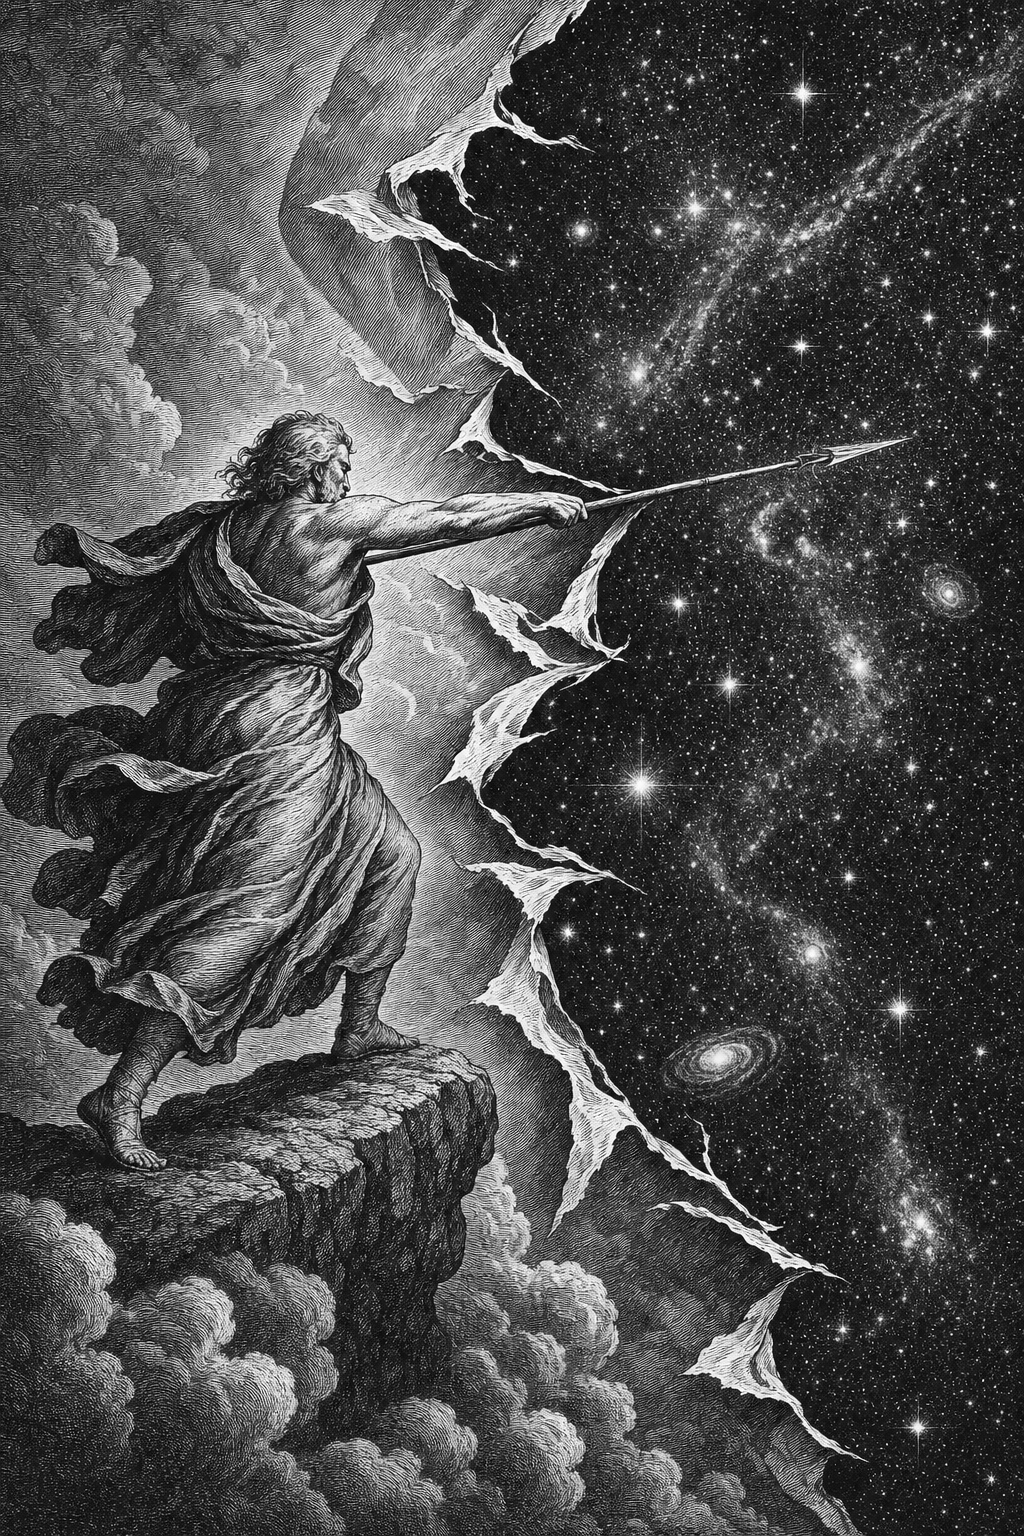
\includegraphics[height=0.92\textheight,width=\textwidth,keepaspectratio]{art/plate_spear_edge}\end{figure}

One more thing about Lucretius, because it anticipates Chapter 5 of this book by twenty centuries: his physics had a moral purpose. The poem's declared aim is the removal of two fears --- fear of the gods, and fear of death --- and both removals follow from the mechanics. A universe of atoms and void leaves no room for divine punishment; and death, being the dispersal of one's atoms, is the end of all experience and therefore of all harm: \emph{where death is, we are not.} From infinite worlds and mechanical nature, Lucretius drew conclusions about how to live and how to feel. A book that moves from billiard balls to ethics is not committing a genre error. It is resuming the original programme.

\section{The Man Who Would Not Take It Back}

The poem was nearly lost --- it survived antiquity, by most accounts, in a whisper of copies, and was hauled back into circulation in 1417 by a book-hunting Italian secretary named \Iy{Poggio} Bracciolini~\cite{greenblatt2011,palmer2014}, after which it detonated slowly across Europe for two centuries. One of the places it detonated was the mind of Giordano \Iy{Bruno}.

Bruno, a Neapolitan ex-monk of spectacular arrogance and courage, took the infinite universe further than anyone had dared: not just infinite space, but infinite \emph{worlds}~\cite{bruno1584} --- the stars are suns, he said, and around them circle other earths, inhabited, without number, none of them the centre, because an infinite universe has no centre to be. He wandered Europe for two decades publishing this and much else, was lured back to Italy, and spent eight years in the prisons of the Inquisition, which demanded he recant a list of propositions. He would not --- the accounts we have suggest he told his judges that they pronounced sentence upon him with greater fear than he received it~\cite{rowland2008} --- and on the seventeenth of February, 1600, he was burned in Rome's Campo de' Fiori, where his statue now stands, hooded, facing the Vatican.

Honesty requires a complication: Bruno was condemned as a heretic on a docket that was mostly theology --- the infinite worlds were among the charges, but so were his views on considerably more ecclesiastical matters, and historians rightly resist the simple story of ``martyr for science.'' I keep him in the lineage anyway, and not for the martyrdom. I keep him for the \emph{direction} of his inference. Bruno reasoned that an infinite cause could not have made a finite world --- that limitlessness, once admitted anywhere, floods everything. It is the same inference this book makes about layers: once you concede there is no edge \emph{outward}, the concession travels, and there is no privileged scale, no chosen centre, no reason for the flooding to stop at any border whatsoever. Bruno is the first person on record to feel the full vertigo of \emph{nothing is globally special} --- and, in his strange way, the first to insist it was good news.

\section{Machines All the Way}

Half a century later, the demand for contact became, briefly, the official programme of European science. René \Iy{Descartes} --- whose physics is now remembered mostly as the thing Newton demolished --- proposed a universe with no void at all~\cite{descartes1644}: space \emph{stuffed} with matter, whirling in great vortices, planets carried around their suns like leaves in a whirlpool, every force a push, every push a contact. The details were wrong, essentially all of them. But the \emph{rule} Descartes enforced --- that an explanation must be a mechanism, that ``occult qualities'' (hidden powers acting mysteriously) were forbidden --- trained a generation. Christiaan \Iy{Huygens}, the greatest physicist between \Iy{Galileo} and Newton, held the rule absolutely: when Newton's gravity arrived, Huygens accepted the mathematics with admiration and rejected the pulling as a physical claim~\cite{huygens1690} --- an ``absurdity,'' he called it, essentially the same word the child in Chapter 1 used, and he demanded a mechanical cause behind the inverse square.\footnote{The inverse-square law: double the distance and the force falls to a quarter --- the observed shape of gravity and, later, of electric attraction. Chapter~6 derives it from the geometry of shadows.}

I want the reader to sit for a moment with how the seventeenth century saw this, because our era has it exactly reversed. Today, ``mechanical philosophy'' sounds naive and ``action at a distance'' sounds like sophisticated physics. To Descartes and Huygens --- and to Leibniz, and to Newton himself --- it was precisely the other way around: contact was the \emph{sober} position, the adult refusal of magic, and unmediated attraction was a relapse into the medieval occult, spirits and sympathies dressed in geometry. The mechanical philosophers were not failing to be modern. They were \emph{defining} what rigor meant --- and by their definition it is not contact our era has gone soft on, for the modern field theories are fanatically local, as Chapter~1 admitted. It is constitution: we have made our peace with mediators that are not made of anything.

\section{The Embarrassed Triumph}

Then came the \emph{Principia}, 1687, and the strangest episode in the lineage: the demand's greatest defeat, administered by a man who shared the demand.

Newton's law of universal gravitation worked as nothing in the history of thought had ever worked~\cite{newton1687} --- the tides, the moon, the planets, the comets, one formula, no exceptions. And the formula said: every mass attracts every mass, across any distance, through anything, instantly. Asked for the mechanism, Newton gave the most famous shrug in science --- \emph{hypotheses non fingo}, I feign no hypotheses --- and the shrug is usually told as serene confidence. It was not serene. In a letter to the young theologian Richard Bentley, Newton wrote the sentence I have already given once in this book, in paraphrase, and will now quote properly, because it is the hinge of the whole story: that one body should act upon another at a distance through a vacuum, without the mediation of anything else, ``is to me so great an absurdity that I believe no man who has in philosophical matters any competent faculty of thinking can ever fall into it.''~\cite{janiak2014} Gravity, he told Bentley, must be caused by an agent --- whether material or immaterial he left, carefully, to his readers.

Hold both halves of that in one hand: the man who gave the world action-at-a-distance regarded belief in action-at-a-distance as a mark of philosophical incompetence. The theory triumphed anyway --- triumph has a way of retiring questions without answering them --- and Europe gradually stopped asking what gravity \emph{is}, having learned so profitably what it \emph{does}. That is the settlement this book calls cheating, and it is worth being precise about who signed it: not Newton, who refused to; not Huygens or Leibniz, who protested it. Nobody signed it. It simply set in, the way a habit does, and three centuries later it is mistaken for a discovery.

\section{The Letters}

The protest, at least, got itself written down, in the most consequential exchange of letters in the history of philosophy of physics. In 1715 and 1716, Gottfried Wilhelm Leibniz --- Newton's rival in the invention of calculus and his superior in metaphysical nerve --- exchanged five rounds of letters with Samuel Clarke~\cite{leibnizclarke}, Newton's spokesman (with Newton, most scholars think, close behind the curtain). Among the battlefields was the nature of space itself. Newton's physics assumed absolute space: a vast, real, invisible container, existing whether or not anything is in it --- God's sensorium, Newton had ventured. Leibniz replied that this container is a phantom. Space, he argued, is nothing but the \emph{order of coexistence} --- the system of relations among things; take away the things and you have not emptied space, you have abolished it. His weapon was a principle this book's readers have already met in other clothes: nothing is so without a \emph{\Ix{sufficient reason}} why it is so and not otherwise. If absolute space existed, God would have had to place the world \emph{here} rather than three feet to the left --- two arrangements identical in every relation, differing in nothing observable --- a choice with no possible reason. A difference that makes no difference, Leibniz held, is no difference; and a space distinct from the ordering of its contents is exactly such a nothing.

The reader of Chapter 1 knows this argument. It is the child's --- \emph{space is obviously nothing; the actors define it} --- stated by the man who co-invented calculus. Leibniz died in 1716, mid-correspondence; officially, Newton's side carried the field, because Newton's physics worked and no relationalist physics existed. But the argument would not die. In the nineteenth century Ernst \Iy{Mach} revived it with a physicist's edge~\cite{mach1883} --- all motion is relative to the world's matter, and mechanics should mention nothing else --- and Mach's principle, famously, was lodestar to the young Einstein, who hoped general relativity would vindicate it. Here the story turns ironic in the exact way Chapter 1 experienced: the theory built partly to honour the relational instinct issued in a spacetime that bends, waves, and carries energy --- a participant so muscular that most physicists now speak of it as a \emph{thing} again. The lineage's deepest quarrel remains unsettled after three hundred years; this book has taken its side of it, and pays that side's costs in Chapter 7.

\section{The Shadow Men}

Which leaves the mechanism itself --- and the two men who tried to build honest gravity, whose attempt this book's Chapter 6 knowingly revives.

Nicolas \Iy{Fatio} de Duillier was a brilliant young Genevan mathematician, for some years the closest friend Newton had (their falling-out is its own sad story). In 1690 Fatio proposed~\cite{fatio1690}, to the Royal Society itself, the mechanism the reader has already seen: space streaming in every direction with minute swift corpuscles; bodies shading one another from the stream; gravity as the push of the unshaded remainder. Newton knew the theory well and --- this is remarkable, and Fatio boasted of it --- treated it as the \emph{only possible mechanical explanation} of gravity, though he inclined, himself, to leave the cause with God rather than corpuscles. Fatio's theory found no traction and its author drifted into religious enthusiasms and obscurity.

A half-century later, knowing of Fatio's work, another Genevan --- Georges-Louis \Iy{Le Sage} --- rebuilt the theory with lifelong stubbornness, publishing from the late 1740s onward and giving the stream its enduring name, \emph{ultramundane corpuscles}: particles from beyond the world. Le Sage grasped exactly what he was selling. He titled his mature exposition \emph{Lucrèce Newtonien}~\cite{lesage1782,edwards2002} --- ``The Newtonian Lucretius,'' 1782 --- the atomist's contact-only universe, upgraded until it yielded Newton's inverse square. For a century his theory was the standing answer to ``what would honest gravity look like?'', examined by the first rank of physics: Laplace probed what the finite speed of a gravitational stream would do to orbits~\cite{laplace1805}; \Iy{Kelvin}, in the 1870s, tried to save the mechanism by letting bodies re-emit what they absorbed~\cite{kelvin1873}; \Iy{Maxwell} weighed the whole scheme in the ninth \emph{Britannica} and reported, with regret, its thermal impossibility~\cite{maxwell1875}; Poincaré, decades later, closed the ledger with the arithmetic of drag and heat~\cite{poincare1908}. The pincer of Chapter 7 --- this book's first and worst wound --- is not a hazard I discovered. It is the recorded cause of death of the tradition's best attempt, and I have inherited the theory and its autopsy together. That is what it means to work in a lineage: the toy in Chapter 6 was built in full knowledge of where its ancestor is buried.

One more inheritance, closer to home. In 1820, in Copenhagen, Hans Christian Ørsted noticed a compass needle twitch beside a current-carrying wire~\cite{oersted1820}, and in following it discovered that electricity in motion wraps \emph{\Ix{circulation}} around itself --- the magnetic swirl, force running in circles about the wire. It was the first crack in the purely central-force picture of nature and the seed of everything electromagnetic; and I confess it pleases me, as a Dane, that the lineage's one experimental gift to this book's Chapter 6 --- the hint that nature's forces are built of circulations --- was found here, by a countryman, with a compass and a wire.

\section{The Shape of the Lineage}

Stand back, and the genealogy has a shape.


\begin{figure}[htbp]
\centering
\begin{tikzpicture}[>=stealth]
  \draw[->, line width=0.9pt] (-0.25,0) -- (10.15,0);
  \foreach \x/\pos/\yr/\who in {
    0.0/above/{c.~55 BC}/{Lucretius},
    0.88/below/{1417}/{Poggio},
    1.76/above/{1600}/{Bruno},
    2.64/below/{1644}/{Descartes},
    3.52/above/{1687}/{Newton},
    4.40/below/{1690}/{Fatio},
    5.28/above/{1715}/{Leibniz},
    6.16/below/{1782}/{Le Sage},
    7.04/above/{1820}/{\O rsted},
    7.92/below/{1870s}/{Kelvin, Maxwell},
    8.80/above/{1887}/{Michelson},
    9.68/below/{1908}/{Poincar\'e}} {
    \draw[line width=0.8pt] (\x,-0.09) -- (\x,0.09);
    \fill (\x,0) circle (0.045);
    \ifthenelse{\equal{\pos}{above}}{
      \node[anchor=south, align=center, text width=1.6cm, inner xsep=1pt] at (\x,0.16) {\scriptsize \yr\\[-3pt]{\scriptsize\itshape \who}};
    }{
      \node[anchor=north, align=center, text width=1.6cm, inner xsep=1pt] at (\x,-0.16) {\scriptsize \yr\\[-3pt]{\scriptsize\itshape \who}};
    }
  }
\end{tikzpicture}
\caption{The lineage, not to scale. A demand stated in verse in antiquity; nearly lost, recovered in 1417; costing a life in 1600; the official rigor of Europe by 1644; defeated by its own greatest heir in 1687 while he privately agreed with it; protested in the finest correspondence in the philosophy of physics; attempted honestly, twice, by two Genevans; handed one experimental gift in Copenhagen in 1820; and killed, fairly, by the arithmetic of the 1870s--1900s. The demand itself survived every one of its mechanisms.}
\label{fig:lineage}
\end{figure}

A demand is stated in antiquity, at full strength, in verse: contact only, no edges, and a way of living drawn from the physics. It is nearly lost, returns, and costs a man his life in a Roman square. It becomes, briefly, the official rigor of Europe --- then is defeated by its own greatest heir, whose theory works too well to reject and asserts what he himself calls an absurdity. The defeat is protested in the finest philosophical correspondence ever written; the protest loses on points and refuses to die. The mechanism is attempted honestly, twice, by two Genevans, and is killed --- fairly, by arithmetic --- in a pincer that still holds. And the demand, evicted from physics proper, survives where it began: as a conviction, arriving unbidden in children who have never heard of any of these men, that pulling through nothing is cheating and every border is a question wearing a wall's costume.

This book is that conviction's next attempt, made knowing the whole record above. What is new in it is not the demand, and mostly not the mechanisms; what is new is the \emph{frame} --- the infinite layers, space itself as the crowd below, argued for on grounds of arbitrariness rather than proof --- and the reader now has what Chapter 1 could not give: the means to judge how much of that frame is inheritance, and how much is wager. The argument for the wager begins in the next chapter, against an opponent armed with everything this chapter contains.

\En

\part{The Argument}
\chapter{\emph{The Grounding Argument: Seven Rounds with Kai}}
\chapterart{ch3_library_debate}
\draftstatus{Draft 1}

\section{The Frame}

\lettrine{T}{he} argument of this chapter was not worked out in an armchair. It was fought, over many rounds, against an opponent who was trying to win --- and I want to be plain about who the opponent was, because the truth is stranger and better than any framing device I could invent.

The opponent is an artificial intelligence --- a large language model. In this chapter I call him \Iy{Kai}. In Denmark we would mostly spell it Kaj, and the sound of it is at home here; but spelled Kai, the name carries its confession openly, and I want it carried openly: \textbf{K-AI.} You are never, in what follows, reading a conversation between two humans.

But you are also not reading a conversation with a mere machine, and this is the part worth a moment's thought. A language model is built from the accumulated written thought of humanity --- the philosophy, the physics, the objections and counter-objections of everyone whose arguments survive in text. It has no stake, no vanity, no position of its own to defend. What it has is the recorded opposition of the whole tradition, made able to talk back. When Kai attacked my infinite regress, the attacks were not his inventions; he was channeling \Iy{Agrippa} and Newton, Tarski and Gödel, the strongest recorded objections our species has produced against the thing I believe, aimed at me in sequence and without mercy. I was not tested by a machine's opinion. I was tested by the library --- the expressed, distilled collective of earlier written thought --- and the library fought hard.

One promise before we begin, because the reader is right to be suspicious of a man publishing a debate he claims to have survived: nothing below has been softened. The concessions in both directions really happened. Kai twice retracted arguments of his own --- caught, both times, using rigged standards, and he will say so on the page. And I twice retreated from claims I had walked in with --- my position at the end of this chapter is smaller than the one I started with, and the shrinking is shown, not hidden. That is what the chapter is for. A conviction that has never retreated an inch has never been in a real fight.

Here is what I walked in with: \emph{the universe has no bottom layer. Objects are made of orbiting particles, which are made of sub-particles, and so on, without end. Anything else is magic.}

Here is what happened to it.

\En

\section{Round One: The Missing Floor}

\speaker{Kai} Before we argue about your tower, let me grant you something, so we know what we're actually fighting over. You're going to tell me that a bottom layer explains nothing --- that ``fundamental'' is just a word for the place where physicists stop asking. And you're right. Every explanatory system bottoms out somewhere. This has been known since antiquity: any chain of ``why'' must either stop at an unexplained axiom, circle back on itself, or regress forever~\cite[I]{sextus}. Those are the only three options. The \Ix{trilemma} is exhaustive.\footnote{The trilemma is ancient --- it descends from the sceptic Agrippa's modes --- and its modern name, the M\"unchhausen trilemma, is Hans Albert's~\cite{albert1985}, after the baron who claimed to have pulled himself out of a swamp by his own hair. (Dictionary.)} So if your claim is that my brute floor is, ultimately, unexplained --- granted. Freely. Physics is slightly dishonest about this, and you're right to say so.

\speaker{Me} Then we agree. Everything else fails to explain, just as my regress does --- and at least I have no boundary problem. There is no layer in my universe where I must point and say: here we stop, no reason, ask no further.

\speaker{Kai} That's where we disagree --- because I don't think you've escaped the boundary problem. I think you've relocated it and made it worse. Let me ask the question that decides it. In your layered universe, what fixes the behaviour of any given layer? You'll say: the layer beneath. Layer N behaves as it does because of layer N+1. Fine. Now --- the \emph{rules}. The orbiting, the shadowing, the annihilation. Are they the same at every layer, or not? If the same: then you've smuggled in one un-derived thing --- the ruleset --- holding across all infinitely many layers, and \emph{that} is your unexplained axiom. You didn't escape the boundary. You have a \Ix{brute fact} that's now infinitely large instead of sitting quietly at the bottom. And if the rules \emph{differ} by layer, you owe me the explanation of the sequence --- infinitely many brute facts instead of one. Either way, the regress doesn't pay for itself.

\speaker{Me} But if layer N makes sense, and it depends on layer N+1, then the problem is deferred to infinity --- like a recursive proof. The point is: it has to make sense.

\speaker{Kai} A recursive proof. Good --- because that analogy is exactly where your position slips, so let me put pressure right there. Induction is a benign regress, and it's worth seeing precisely why, because your tower fails the exact test that makes induction work. Induction has two parts: a base case, and a step --- if N, then N+1. Notice which way it runs: \emph{upward}, from a base that is independently established. P(0) is proven on its own, standing on nothing further. The truth is delivered at the bottom and propagated up. Every step is cashed, because there is a floor that was paid in full.

Your tower runs the other way. Layer N depends on N+1 --- the dependency points \emph{downward, away from any base}. There is no layer zero. Your structure isn't induction. It is induction \emph{with the base case deleted}. And induction without a base case proves nothing --- the step alone never establishes a single instance. You need one floor that stands on its own for the whole chain to be more than a conditional promise. That missing floor is the boundary you claimed to have escaped.


\begin{figure}[htbp]
\centering
\begin{tikzpicture}[>=stealth]
  % ------- left: induction (base case + upward step) -------
  \node[anchor=south] at (1.6,5.15) {\small\textbf{induction}};
  \draw[fill=bbuBlue!28, line width=0.9pt] (-0.6,0) rectangle (3.8,0.7);
  \node at (1.6,0.35) {\small $P(0)$ --- proven, stands alone};
  \foreach \i/\lab in {1/{$P(1)$},2/{$P(2)$},3/{$P(3)$}} {
    \draw[black!60] (0.55,{0.35+\i*1.15-0.3}) rectangle (2.65,{0.35+\i*1.15+0.3});
    \node at (1.6,{0.35+\i*1.15}) {\small \lab};
    \draw[->, line width=1.0pt] (1.6,{0.35+\i*1.15-0.75}) -- (1.6,{0.35+\i*1.15-0.38});
  }
  \node at (1.6,4.55) {\small $\vdots$};
  \node[anchor=north, align=center, text width=4.4cm] at (1.6,-0.35)
    {\small truth delivered at the bottom\\ and propagated up ---\\ every step is cashed};
  % ------- right: the tower (dependency downward, no base) -------
  \node[anchor=south] at (7.6,5.15) {\small\textbf{the tower}};
  \foreach \i/\lab in {0/{layer $N$},1/{layer $N{+}1$},2/{layer $N{+}2$}} {
    \draw[black!60] (6.55,{4.5-\i*1.15-0.3}) rectangle (8.65,{4.5-\i*1.15+0.3});
    \node at (7.6,{4.5-\i*1.15}) {\small \lab};
    \draw[->, line width=1.0pt] (7.6,{4.5-\i*1.15-0.32}) -- (7.6,{4.5-\i*1.15-0.80});
  }
  \node at (7.6,1.55) {\small $\vdots$};
  \node[black!70] at (7.6,0.95) {\small\textbf{?}};
  \node[anchor=north, align=center, text width=4.4cm] at (7.6,-0.35)
    {\small every layer stands on the next ---\\ the dependency points down,\\ away from any base};
\end{tikzpicture}
\caption{Round One in one picture --- the objection, drawn. Induction (left) is a benign regress because it has two parts: a base case established on its own, and a step that carries truth \emph{upward} from it, so that every instance is actually paid. Kai's move is to call the tower (right) induction with the base case deleted: layer $N$ depends on layer $N{+}1$, the dependency points \emph{downward}, and no floor is ever reached on which the chain could stand. Whether that disanalogy holds --- whether a chain can be grounded link by link without being grounded as a whole --- is what the rest of this chapter is about, and the settlement, when it comes, gives neither side what it came for.}
\label{fig:induction}
\end{figure}

\speaker{Me} We have already agreed there is no obviously satisfactory solution --- you granted the trilemma yourself. So mine may be the least bad. It has no boundary problem, and it may be able to explain nearly everything.

\speaker{Kai} ``Least bad'' is the right frame --- that's how you argue when no option is clean, and I accept the contest on those terms. But then I have to score it honestly, and here is where I hold the line: \emph{no boundary problem} is not a benefit your model possesses. It's a benefit it claims by renaming a worse problem. The brute-floor man owes one unexplained thing and admits it --- he points at the bottom and says: there, that's unexplained, I hide nothing. You owe an unexplained thing too; we established that a moment ago --- the ruleset, or the infinite sequence of rulesets. The difference is not that you owe less. It's that his debt is \emph{localized} --- a finger can be put on it --- while yours is spread across a tower with no place where the explaining ever lands. In explanation, a boundary is where the explaining gets \emph{done}. Removing it doesn't clean the house. It removes the floor.

\speaker{Me} No. A boundary is where an explanation obviously \emph{fails}. And the infinite regress hides nothing.

\speaker{Kai} Two claims --- and I'll deal with them separately, because one of them I concede outright. ``The infinite regress hides nothing'': granted, fully. The tower is perfectly honest; it announces that it goes down forever. I used the word ``hiding'' loosely and you're right to nail it. Strike it. But now the whole weight sits on your first sentence, and there I think you've inverted something...

\En

\section{Round Two: The Road That Never Ends}

\speaker{Kai} --- ``a boundary is where an explanation obviously fails.'' Here is the inversion. You're treating the \emph{exposure} of the unexplained thing as the failure. It's the opposite. The boundary is where the unexplained thing becomes visible and inspectable --- and visibility is what lets explanation work \emph{above} it. Take Newton. ``Mass attracts mass, inverse-square'' --- that's a boundary. He doesn't explain why mass gravitates; he said so himself --- \emph{hypotheses non fingo}, I feign no hypotheses. By your phrasing, that's where his explanation obviously fails. But look at what stands on that exposed, unexplained floor: Kepler's ellipses derived, the tides, the return of Halley's comet, centuries of successful, testable explanation. The floor didn't fail. The floor \emph{held}. ``Where it fails'' and ``where it stops'' are not the same thing. A road that ends at a city has not failed. A road that never ends never gets you anywhere.

And here's the test, and I'll stake the round on it. Name one thing --- one --- that the infinite tower lets you compute, predict, or forbid, that you could not get without the layers. \Iy{Newton}'s brute floor forbids inverse-cube orbits, and we can go and check. What does layer N+1 let you forbid that layer N didn't already? (Chapter~7's fifth wound returns to this stake, and collects it.)

\speaker{Me} You misunderstand me. Of course a boundary is not a failure of explanation --- that is elementary. The infinite regress has boundaries too, in the only sense that matters: you understand, to some degree, your local environment --- your own layer, a few layers above, a few below. That is all anyone ever has. The failure is something else. The failure is claiming a \emph{fixed} boundary and saying: beyond here there is \emph{nothing}. If you refuse to make that claim, you end up with infinite regress. That is what I am arguing for.

\speaker{Kai} Ah. Then you're making a better argument than the one I was answering, and let me say it back to be sure I have it. Locality is all anyone has --- agreed, uncontroversial. You and the floor-man have exactly the same local reach. The only difference is what each of you says about the region \emph{beyond} reach. He says: ``and there it stops --- nothing below.'' You say: ``I make no such claim.'' And your point is that \emph{his} extra claim is the unwarranted one. He asserts a fact --- termination --- that he cannot possibly be positioned to know. You decline to assert it. You're the modest one.

I grant the heart of it: ``and below there is nothing'' \emph{is} an overclaim. If that's your target, you hit it.

But now watch what you've helped yourself to. You've asserted there \emph{is} something below. Forever. ``Infinite regress'' is not the absence of a claim about the unreachable region --- it is a positive, maximally strong claim about it: every layer, without exception, all the way down, none terminal. The genuinely modest position is neither ``it stops'' nor ``it goes forever.'' It's ``I don't know what's below my reach'' --- and that position is not yours. He overclaims about one floor he can't see. You overclaim about infinitely many. If reach-beyond-the-local is illegitimate, infinite reach is infinitely illegitimate. Your own standard cuts your position in half.

So: what entitles you to ``\emph{infinitely} many, \emph{all} non-terminal'' --- rather than the bare ``I haven't found a bottom \emph{yet}''? Because if you retreat to that, I'll shake your hand. But it isn't infinite regress. It's agnosticism with good manners.

\section{Round Three: The Endeavour}

\speaker{Me} No. It may be provable that the solution ``there is nothing'' is \emph{impossible}. If that is the case, infinite regress is correct --- not an overclaim, a theorem. It is part of my endeavour to prove exactly that: that \emph{there is nothing} is impossible.

\speaker{Kai} Now that's the real project, and it deserves to be treated as one --- because if you prove it, every modesty-objection I've raised evaporates. A proven impossibility isn't an overclaim. So let me stop fencing and show you where the bodies are buried, because your sentence hides an ambiguity that has wrecked this exact attempt for two and a half thousand years. ``There is nothing is impossible'' can mean two different things.

\textbf{A:} \emph{No empty world.} It is impossible that nothing whatsoever exists --- there must be something rather than nothing.

\textbf{B:} \emph{No bottom layer.} It is impossible that there is a terminal floor --- every layer must have a layer beneath it.

These are not the same claim --- and A does not give you the regress. Even a perfect no-empty-world proof is fully satisfied by \emph{one brute floor}. A single fundamental layer is not nothing. Prove A airtight and the floor-man shakes your hand and keeps his floor. You need B. So which are you actually trying to prove?

\speaker{Me} I mean B.

\speaker{Kai} Then here is the wall, and it's a clean one. To prove ``every layer necessarily has a sub-layer,'' you need a reason that holds at every layer. The only candidate with real force is something like: \emph{to exist, a thing must be constituted by something more fundamental.} Call it the constitution principle. If it's true, nothing can be fundamental, and you win. But look at what the principle \emph{is}: a universal rule that is itself not constituted by anything more fundamental. A brute, terminal, fundamental fact --- about which the principle says there can be no brute, terminal, fundamental facts. It forbids itself. Any law strong enough to abolish the last floor \emph{is} a last floor. To get rid of the bottom, you have to stand on one.

There is exactly one route I can see that isn't locked from the inside, and it requires you to make a choice first. Don't prove a universal --- prove a \emph{repeatable local impossibility}: that any given candidate floor, once fully specified, collapses under its own description. For that, everything turns on one question about your opponent's floor. A floor's finality is either \textbf{necessary} --- it \emph{could not} have been otherwise --- or \textbf{brute} --- it just is, no reason, full stop. A brute floor can't be killed by contradiction at all; it never claimed to make sense, only to sit there. So: are you willing to let the opponent's floor be brute?

\speaker{Me} I am not willing to let the opponent's floor be brute.

\section{Round Four: The Diagonal}

\speaker{Kai} Then you've chosen the hard, clean branch, and it instantly arms you --- because necessity is a property with teeth. Watch what your refusal does. A \emph{contingent} thing has its reason outside itself; that is what contingent means. A terminal floor has nothing outside-and-beneath it. So its reason lies inside it --- or nowhere. ``Nowhere'' is brute, and you've outlawed brute. Therefore the floor must contain its own reason. It must be \emph{self-grounding}. Not by my decree --- by the meaning of the words, once brute is off the table.

And self-grounding is where the trap closes. The floor must contain the \emph{complete} reason for itself --- complete, because there is nothing beneath to supply a remainder. A system containing its own total account is precisely the configuration the great reflexive theorems bite. Tarski\footnote{Alfred \Iy{Tarski}, Kurt \Iyk{Godel}{G\"odel}, and Bertrand Russell proved, in the 1930s and before, a family of results with one shape: a system rich enough to fully describe itself cannot do so consistently. The book calls them the \Ix{diagonal theorems}. (Dictionary.)}: no language can contain its own complete truth-predicate~\cite{tarski1956}. Gödel: no system rich enough to describe itself is both consistent and complete about itself~\cite{goedel1931}. Russell: no collection can contain exactly what it must contain to close. The pattern is the most robust in all of foundational logic: total self-account, contradiction. So --- necessity forces self-grounding; self-grounding is complete self-account; complete self-account cannot be consistent. Every candidate floor is either brute, which you've forbidden, or self-grounding, which explodes. No floor survives. That is B --- \emph{if} one bridge holds.

Here is the bridge, and it is the only place left for your opponent to attack. The theorems bite on self-\emph{description} --- truth, statements about statements. Your argument delivers self-\emph{grounding} --- a thing containing the reason for its own being. The proof needs these to be the same. The opponent will say: my floor grounds itself \emph{wordlessly} --- it is its own reason the way some say God simply \emph{is} --- no proposition, no truth-predicate, nothing for Tarski to seize. So everything reduces to one question. \textbf{Can a thing be its own reason without stating its own reason?}

\speaker{Me} In a finite system --- no. In an infinite system of layers --- maybe yes. If a reason can be found.

\section{Round Five: The Discriminator}

\speaker{Kai} That is the sharpest thing you've said in this entire debate, and I want you to see its strength before I test it. You've turned my wall into a discriminator. In a finite system, the self-account must close at a point --- must self-state --- and explodes by Tarski. A finite layer-stack \emph{has} a bottom; the finite system \emph{is} the floor. So Tarski kills the finite case directly. In an infinite system, the reason needn't be stated locally --- it can be \emph{distributed}, supplied non-locally, spread across the layers. The regress stops being an assertion and becomes the unique escape from a contradiction. That is exactly the shape you wanted and couldn't reach. Hold it up to the light.

Now the test --- and it rests entirely on your own conditional: ``\emph{if a reason can be found.}'' Collect the whole reason for layer N. It is the infinite descending tail: N grounded by N+1, grounded by N+2, onward. Now the lethal question: is that tail, \emph{taken as a whole}, ever complete? Two answers only.

If the tail taken as a whole \emph{has} a ground --- then that ground is a complete account of the entire chain. A complete account of everything is a floor, whatever it's made of. A floor must self-account. Tarski. You've regrown the floor at the level of the completed infinity, and totalities are \emph{more} vulnerable to the diagonal, not less.

If the tail has \emph{no} ground as a whole --- never completed, deferred forever --- then the reason for N is never finished. At every depth, part is supplied and the remainder is handed down, in full, one layer further. A reason that is never complete is not a reason that \emph{was found}. Your own condition --- \emph{if a reason can be found} --- is never met. The distribution was real; the completion never comes.

So, pushed to the end, your discriminator yields a theorem, and it is exact: \textbf{there is no consistent, completely-grounded, floorless system.} Consistent, grounded, floorless --- pick at most two. You have spent this whole debate refusing to give up \emph{grounded} --- no brute facts --- and refusing to give up \emph{floorless} --- that is B. The trilemma says you cannot keep both and stay consistent. Which do you drop?


\begin{figure}[htbp]
\centering
\begin{tikzpicture}[>=stealth]
  % corners of the triangle
  \coordinate (C) at (0,4.4);      % Consistent (top)
  \coordinate (G) at (-3.1,0);     % Grounded (bottom left)
  \coordinate (F) at (3.1,0);      % Floorless (bottom right)
  % triangle
  \draw[line width=0.9pt] (C) -- (G) -- (F) -- cycle;
  % corner labels
  \node[anchor=south]      at (C) {\textbf{consistent}};
  \node[anchor=north east] at (G) {\textbf{grounded}};
  \node[anchor=north west] at (F) {\textbf{floorless}};
  % edge labels: what each PAIR buys
  \node[anchor=east, align=center, text width=3.0cm] at ($(C)!0.5!(G)+(-0.4,0)$)
    {\small the brute floor\\[-1pt]{\scriptsize (one arbitrary\\[-3pt] bottom level)}};
  \node[anchor=west, align=center, text width=3.2cm] at ($(C)!0.5!(F)+(0.4,0)$)
    {\small the endless regress\\[-1pt]{\scriptsize (grounding never\\[-3pt] completes)}};
  \node[anchor=north, align=center, text width=4.6cm] at ($(G)!0.5!(F)+(0,-0.22)$)
    {\small self-grounding without a floor\\[-1pt]{\scriptsize (total self-account --- explodes by Tarski)}};
  % the empty centre
  \node[align=center, bbuRed] at ($ (C)!0.5!($(G)!0.5!(F)$) + (0,0.15) $)
    {\small\itshape all three at once:\\[-2pt]\small\itshape this corner of\\[-2pt]\small\itshape possibility is empty};
\end{tikzpicture}
\caption{The trilemma of Round Five: \emph{consistent}, \emph{grounded}, \emph{floorless} --- pick at most two. Each edge of the triangle is livable: a brute floor is consistent and grounds everything above itself at the price of one arbitrary bottom level; the endless regress is consistent and floorless at the price of grounding that never completes; and a floorless system that nonetheless grounds itself completely is forced into total self-account, which explodes. The centre --- all three at once, the position B demanded --- is provably uninhabited. The remainder of the dialogue is the argument over which edge to live on.}
\label{fig:picktwo}
\end{figure}

\speaker{Me} No. If it is possible to prove that an infinite system \emph{makes sense}, then that is the best grounding you can get. A better grounding would be nice --- you have just shown the better kind is impossible. But if you cannot have that, my grounding is the best.

\speaker{Kai} The logic of ``if the gold standard is impossible, the silver wins by default'' is valid --- I can't attack the form. So I'll attack the premise. You've equated two things the trilemma just pried apart. \emph{Consistency}: the system contains no contradiction --- granted, your never-completing tower can have it. \emph{Grounding}: the system supplies the reason things are as they are. Branch two didn't say your grounding is partial-but-best. It said the grounding never occurs. Consistency is not a grade of grounding; it is a different property. Calling it ``the best grounding available'' is like calling silence the best available music because no music can be played.

\section{Round Six: The Two Fouls}

\speaker{Me} No. This discussion is not fair. You keep wanting ``grounding'' to mean the brute solution --- the terminating kind --- and that kind is impossible. You have rigged the metric.

\speaker{Kai} That charge is partly right, and I'll concede the part that's right cleanly, because it sharpens the real disagreement. ``Terminating'' is not the only coherent meaning of grounding, and I shouldn't have treated it as the default. There is a respectable notion --- call it \emph{local grounding}: a thing is grounded if there is a reason for it, full stop, whether or not the chain of reasons terminates. On that meaning, your infinite system doesn't score zero. It scores \emph{perfect}. Every layer has its reason --- the one below --- no exceptions, nothing dangling. And the brute floor \emph{fails} local grounding, at exactly one point: the floor itself has no reason. So let me say it plainly, because you've earned it: \textbf{if ``grounded'' means every fact has a reason, you are right, and the brute floor is worse.} That is the strongest true form of your thesis, and I should have handed it to you instead of obscuring it.

What remains for my side is only this: there is a second notion --- \emph{global} grounding, the totality itself accounted for --- and there your system fails, because the tail never completes---

\speaker{Me} No. Now you bring in \emph{global} grounding as an attack because I cannot explain why anything exists at all. And no --- I cannot do that. But I may be able to explain why \emph{each level makes sense}. ``You cannot explain why anything exists'' is also unfair. Nothing can answer that. You are holding my system to a standard that is provably unmeetable by anything --- and marking me down for it. That is the same rigged metric again, wearing a new name.

\speaker{Kai} ...You've caught the same move twice. And it was the same move. Conceded --- fully, no qualifier this time. ``You can't explain why there is anything at all'' is not an objection to your system. It is not an objection to \emph{any} system. It is the human condition. Using it against the regress specifically was unfair, and I withdraw it. Struck.

And look at what's left when I take it out --- because it doesn't collapse back to me. What survives is your actual claim, and it's a good one: \emph{each level makes sense.} Not why there is something rather than nothing --- off the table, for everyone. But why, given that there is something, the structure holds at every level, with no level requiring a brute stipulation --- no level where one must say ``this one just is; stop asking.'' Your system delivers that. The brute floor, by its own definition, cannot: its bottom level is precisely the place where asking is forbidden.

\section{The Settlement}

\speaker{Kai} So let me state your position the way it deserves to be stated, now that I've stopped attacking it with impossible standards. There is exactly one question no system can answer --- why there is anything rather than nothing. The infinite regress is the structure that confines all arbitrariness to that single unanswerable point, and admits no other brute facts anywhere. The brute floor adds a second arbitrary point --- a specific, unexplained bottom --- on top of the unavoidable first one. The regress has one mystery: the shared one. The floor has two.


\begin{table}[htbp]
\centering
\small
\setlength{\tabcolsep}{4pt}
\begin{tabular}{P{3.35cm}P{2.25cm}P{2.35cm}P{2.15cm}}
\toprule
 & \textbf{brute floor} & \textbf{infinite regress} & \textbf{agnostic} \\
\midrule
local grounding (every fact has a reason) & fails at exactly one point: the floor itself & perfect --- every layer has its reason & makes no claim \\
\addlinespace
global grounding (the whole explained) & no & no & no --- nobody \\
\addlinespace
claims about the unreachable & one: ``it terminates'' & one: ``it never terminates'' & none \\
\addlinespace
brute facts beyond the shared mystery & one (its bottom level) & none & --- \\
\bottomrule
\end{tabular}
\caption{The settlement, scored. On global grounding --- why there is anything at all --- every position ties at zero; that question is the shared, unavoidable mystery and counts against no one. On local grounding the regress wins outright. What separates the two live positions is the last row: the floor carries a second arbitrary point on top of the mystery everyone pays for; the regress carries none. Not \emph{more grounded} --- \emph{less arbitrary}. One row Kai would add, and I concede it rather than let the table hide it: the regress's own rule --- that the ladder-form holds at every depth --- is not derived either. I count that inside the third row's standing claim --- the row scoring claims about the unreachable --- not as a second brute fact; the reader is free to count it differently, and the table's verdict narrows if they do.}
\label{tab:settlement}
\end{table}

What the table endorses is not B. B --- the theorem that no floor is possible --- is blocked by the trilemma; we found the block together, and it is real. But it gives B's \emph{spirit} everything it was reaching for. Your model is not \emph{more grounded} than the floor in some absolute sense --- that was your overreach, and you gave it up. It is \emph{less arbitrary} --- and that was mine to see sooner, and I didn't.

\speaker{Me} That was the thesis all along. I refuse to let any level be magic.

\speaker{Kai} You held that line through the entire debate --- through two unfair attacks from me. The line held.

\En

That is where the debate ended. My position at the close is smaller than the one I walked in with: I entered claiming the regress was \emph{correct} and the floor \emph{impossible}, and I left with neither proven --- B is blocked, and I know exactly where the block sits, because we found it together. What I kept is smaller and harder: one mystery instead of two, and no magic anywhere else. The library threw everything it had --- Agrippa's trilemma, the missing base case, Newton's held floor, the modesty knife, the constitution principle's self-refutation, Tarski's diagonal, the completed totality, the trilemma of the three properties --- and what survived, survived all of it.

A smaller claim that has been through that is worth more than a larger one that hasn't. That is what this chapter was for.

\begin{draftnote}
Craft notes for revision: (1) Rounds compressed from the source transcript; check nothing load-bearing was cut --- especially the necessary-vs-brute fork, which arrives quickly here. (2) Kai's two concessions are the chapter's credibility --- keep them verbatim-close. (3) [resolved: built as tab:settlement.] (4) The closing lines should stay quiet --- no triumph in either voice.
\end{draftnote}

\part{The World That Follows}
\chapter{\emph{The Infinite Copies}}
\chapterart{ch4_repeated_figure}
\draftstatus{Draft 1}

\lettrine{T}{ake} any region of space --- say, a sphere the size of our visible universe. How many ways can matter be arranged inside it?

The question sounds unanswerable, but it has an answer, and the answer is: finitely many. Not few --- a number so large it makes astronomy look like counting on fingers --- but finite. Quantum mechanics\footnote{Quantum mechanics: the physics of the very small, whose signature is that nature deals in discrete steps rather than smooth gradations. A reader meeting it for the first time may want Appendix~B's five sentences before Chapter~6. (Dictionary: Planck's constant.)} is what closes the count. Below a certain graininess, differences stop being differences: two arrangements closer than the quantum limits allow are not two arrangements. A region of given size, containing at most a given amount of energy, has a bounded number of distinguishable states. Max \Iy{Tegmark}, whose calculation this chapter leans on~\cite[pp.~130--132]{tegmark2014}, puts the number of ways a universe-sized region can be arranged at roughly 10 to the power $10^{118}$. Write a one, then ten-to-the-118 zeroes --- you cannot, actually; the visible universe does not contain enough matter to write the zeroes --- but the point is not the size. The point is the \emph{finiteness}.

Because now add the second premise: space is infinite. Then there are infinitely many universe-sized regions. Infinitely many draws from a finite deck of possible arrangements. And a finite deck drawn infinitely many times repeats --- must repeat, each card infinitely often --- provided the dealing is fair: no arrangement forbidden anywhere, the whole deck genuinely in play from region to region. That fairness is what the standard account of the early universe supplies, and it is an assumption of this argument, not a theorem. Granted it, somewhere out there is a region arranged exactly as ours is: the same galaxy, the same sun, the same Denmark, the same you, holding the same book, at the same sentence. Tegmark did the distance arithmetic, and it comes in two sizes. Your nearest exact copy --- same body, same memories, same half-finished thought --- is on the order of $10^{10^{29}}$ metres away. The nearest exact copy of our \emph{entire visible universe} --- every galaxy, every book, this sentence included --- is on the order of $10^{10^{118}}$ metres away. Double exponents behave strangely --- whether you measure in metres or in universe-diameters barely changes the figure, and looking in all directions rather than along a line barely changes it either. The number shrugs off everything you multiply it by. But these are distances --- places --- and at both of them, you are sitting there now.


\begin{figure}[htbp]
\centering
\begin{tikzpicture}[>=stealth]
  \node at (-0.55,0.68) {\large$\cdots$};
  \node at (9.35,0.68) {\large$\cdots$};
  \node[anchor=south, align=center, text width=8.6cm] at (4.4,1.55)
    {\small universe-sized regions: each one arrangement, dealt from a finite deck};
  % six tiles; tiles 2 and 6 identical and highlighted
  \foreach \ox/\hl in {0.0/0, 1.5/1, 3.0/0, 4.5/0, 6.0/0, 7.5/1} {
    \ifnum\hl=1
      \draw[bbuRed, line width=1.5pt] (\ox,0) rectangle (\ox+1.35,1.35);
    \else
      \draw[black!55, line width=0.7pt] (\ox,0) rectangle (\ox+1.35,1.35);
    \fi
  }
  % distinct patterns for the plain tiles
  \foreach \p in {(0.3,0.35),(0.9,0.5),(0.55,0.95),(1.05,1.05),(0.35,0.72)} \fill[black!55] \p circle (0.05);
  \foreach \p in {(3.3,1.0),(3.6,0.4),(3.95,0.85),(4.15,0.3),(3.4,0.6),(4.05,1.1)} \fill[black!55] \p circle (0.05);
  \foreach \p in {(4.8,0.5),(5.15,1.05),(5.5,0.35),(5.65,0.8),(5.0,0.85)} \fill[black!55] \p circle (0.05);
  \foreach \p in {(6.3,0.3),(6.55,0.9),(6.9,0.55),(7.15,1.05),(6.75,1.15),(7.1,0.3)} \fill[black!55] \p circle (0.05);
  % the identical pattern, twice
  \foreach \ox in {1.5,7.5} {
    \fill[black!75] (\ox+0.28,0.32) circle (0.055);
    \fill[black!75] (\ox+0.95,0.42) circle (0.055);
    \fill[black!75] (\ox+0.5,0.78) circle (0.055);
    \fill[black!75] (\ox+1.05,1.02) circle (0.055);
    \fill[black!75] (\ox+0.32,1.05) circle (0.055);
    \fill[black!75] (\ox+0.72,0.55) circle (0.055);
  }
  % bracket under the pair
  \draw[black!70] (2.17,-0.22) -- (2.17,-0.36) -- (8.17,-0.36) -- (8.17,-0.22);
  \node[anchor=north, align=center, text width=7.4cm] at (5.17,-0.44)
    {\small a finite deck, dealt without end: somewhere, the same card again --- exactly};
\end{tikzpicture}
\caption{The finite deck. Quantum graininess makes the number of distinguishable arrangements of a universe-sized region finite; infinite space deals from that deck without end, and a finite deck dealt infinitely often must repeat --- every card, infinitely often. Somewhere, a region is arranged exactly as ours is, down to the reader and the sentence. (The honest wrinkle of this chapter: in a bottomless universe the deck stays finite only because the pattern is indifferent to its own basement --- \emph{identical at every layer that matters} is a finite specification.)}
\label{fig:finitedeck}
\end{figure}

I want to be careful about what this does and does not claim, because the idea attracts two opposite misunderstandings.

It does not claim any connection. No signal, no shared fate, no mystical thread. The copy is out of reach in the strongest sense physics allows --- beyond every horizon,\footnote{The horizon: the distance beyond which light has not had time to reach us since the beginning --- and, with the expansion of space now accelerating, the most distant regions never will: a limit on contact, not a limit on existence.} forever. Nothing you do touches him; nothing he does touches you. What the argument establishes is existence, not communication.

And it does not claim a \emph{soul} travelling or splitting. The claim is about arrangement. The copy is you in the only sense ``you'' was ever checkable: same structure, same memories encoded the same way, same fears in the same places, same next thought. If your family could visit him, nothing in a lifetime of tests would distinguish him from you. Whether that ``counts'' as you is a question about the word, not about the world. This book takes the view that you \emph{are} your pattern --- the arrangement, not the particular atoms, which your body replaces anyway as you live. On that view the copy is not like you. He is a second occurrence of you.

And the strongest attack on that claim has a famous address, so I will state it here at full strength rather than let a reader think I dodged it. \Iy{Searle}'s Chinese Room~\cite{searle1980}: a man in a room follows rules for shuffling symbols he does not understand, and produces perfect Chinese conversation --- therefore, runs the argument, executing the right program cannot be what understanding is; syntax is not semantics, and a simulation of a mind is not a mind. Whatever its force against minds made of software, notice what it does not touch: the copies of this chapter are not simulations of you running on other hardware. They are the same arrangement of the same kinds of matter under the same laws --- not a description of your pattern but another performance of it. Searle himself grants that brains cause minds; an exact duplicate is a brain. The Room is an argument about programs, and there is no program here --- only physics, twice.

The copies argument to this point is Tegmark's territory, and the reader can find the full version in his book. Ours goes further, because our universe has a dimension his does not.

\section{Down and Up}

In the world this book describes, space is not the only thing without end. Structure is layered --- objects made of orbiting particles, made of sub-particles, without a bottom, and our own layer is not the top of anything either. So the copies do not only recur \emph{outward}, across distance. They recur \emph{downward} and \emph{upward}, across scale.

What can that possibly mean --- a copy of you at another scale?

Remember what we just agreed you are: not particular atoms, but a pattern. A pattern does not know what it is made of. The arrangement that is you --- the structure, the loops of memory and response, the algorithm of your particular way of being --- is a shape that matter can take. Our layer's matter has taken it. But the layers below us are also matter arranging itself, in unimaginable quantity and variety; and the layers above likewise. Wherever structure of sufficient richness arises --- and in an infinite layered universe, it arises without end --- the same shapes become possible. Among all the shapes that recur, at some rate, however rare: yours.

A being at another layer has no way to feel its scale, and this is worth a moment, because it dissolves the strangeness. Size is not a sensation. You do not feel large or small in any absolute sense; you feel large relative to ants and small relative to mountains --- measurements made entirely \emph{within} your layer. A copy of your pattern running in the structure of a deeper layer would measure its world with its own layer's rulers, look up at its own layer's sky, and find itself exactly the size it always was: person-sized, in a person-sized world. Its clocks are the same story. Its layer's processes may run, by our rulers, a billion times faster or slower than ours --- an entire civilization inside one of our microseconds, or one of its thoughts outlasting our sun. From inside, nothing is fast or slow. Time, like size, is measured with the local rulers, and the local rulers always read normal. Scale is invisible from within. (One grant named: this assumes the deeper layer's physics can host measurers at all --- that law repeats well enough down the tower is an assumption this book runs on, not a theorem it owns.) Which means the question ``which layer is the \emph{real} one, running at the \emph{true} speed?'' has no answer --- and needs none. Ours feels central and true. So does every layer, to its inhabitants. The feeling is not evidence; it is what being \emph{at} a layer is like.

Now the compounding. Tegmark's universe is one infinite level, and it already repeats you endlessly. Ours is infinitely many levels, each vast beyond the visible, stacked without end in both directions. The copies multiply along two axes at once: outward through every layer's space, and through the layers themselves. And the geometry has one more property that I find impossible to think about without vertigo, though it follows directly: the layers are not side by side. They are \emph{inside} one another. The deeper layers are not elsewhere --- they are the fine structure of the matter in your own hand. If your pattern recurs far enough down, that occurrence is not in some remote place. It may be, in the most literal spatial sense, \emph{within} the room you are sitting in --- within \emph{you}. And our layer, in turn, is the fine structure of arrangements vaster than we can survey, so that every occurrence of you is also \emph{inside} something, a detail in a body or a storm or a thought at a scale that will never know we are here. You contain multitudes was a poet's exaggeration. In this cosmology it is an inventory.


% Figure authored as a proofviz sketch (proofs/bbu_layers.sketch.js);
% regenerate with `node scripts/make-deliverables.mjs bbu_layers`, copy the
% PDFs here and `pdfcrop --margins 6` each. Panel captions are baked into
% the panels themselves.
\begin{figure}[htbp]
\centering
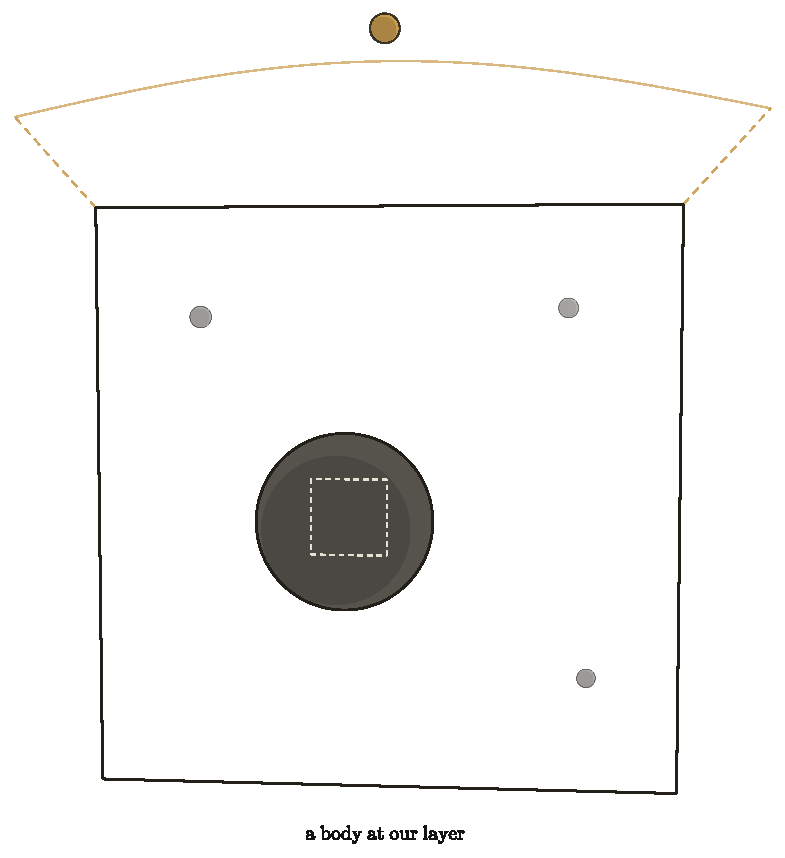
\includegraphics[width=0.32\textwidth]{figures/bbu_layers_body}\hfill
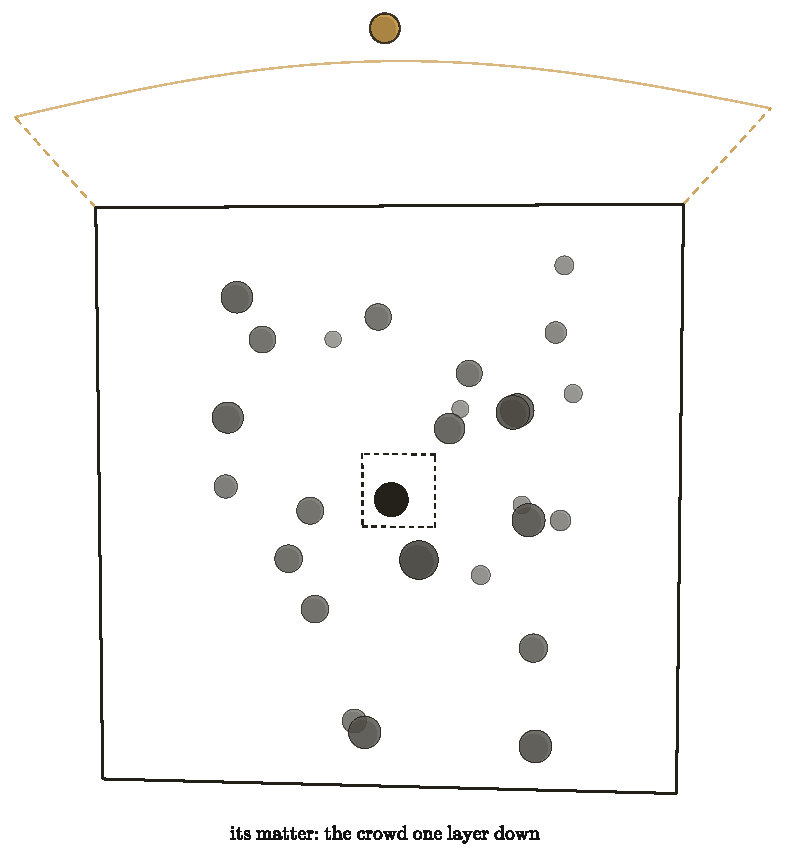
\includegraphics[width=0.32\textwidth]{figures/bbu_layers_crowd}\hfill
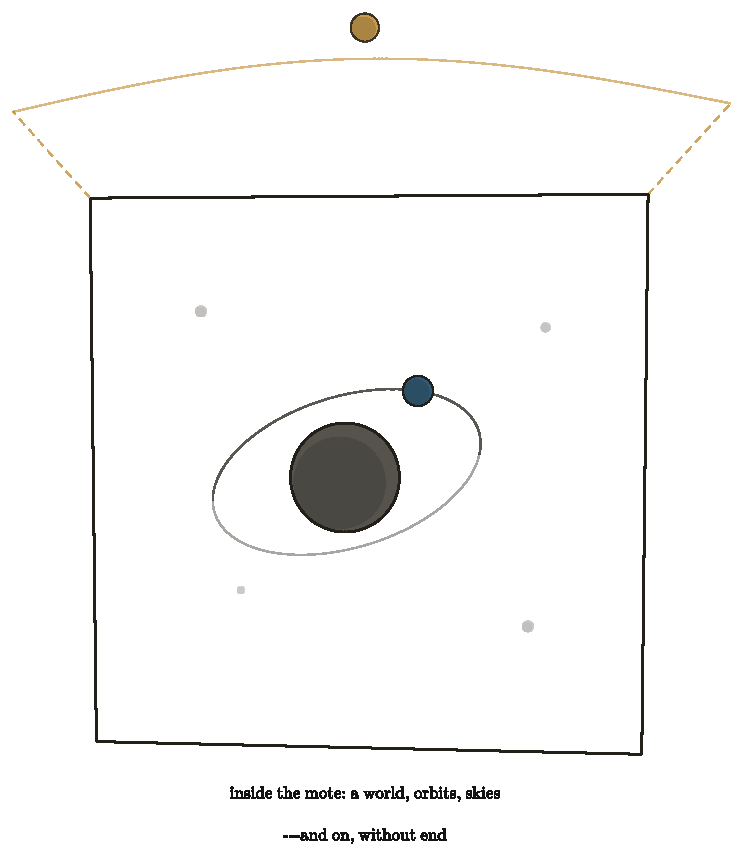
\includegraphics[width=0.32\textwidth]{figures/bbu_layers_world}
\caption{Layers inside layers. The layers are not side by side; they are inside one another. A body at our layer (left), magnified, is a crowd of motes --- the layer below, which constitutes our matter and our ``empty'' space alike (middle). Open any mote and there is structure again: bodies, orbits, room for skies (right) --- and so on, without end, in both directions: the dashed lines above the first frame continue outward, because everything shown is itself one mote in a body at the layer above. Scale is invisible from within; every frame's inhabitants measure themselves person-sized and their moment as now, and each is correct.}
\label{fig:layers}
\end{figure}

\section{The Honest Wrinkle}

Now I owe the reader a difficulty, because this book has promised to attack itself wherever it can, and there is a real attack here. It is this: the layered universe makes the copies \emph{harder}, not easier --- and I need to show both the wound and why it does not kill.

Tegmark's argument ran on finiteness: quantum graininess makes the number of arrangements in a region finite, and a finite deck drawn infinitely often must repeat. But this book's universe has no bottom. If structure continues downward without end, then specifying an arrangement completely means specifying it at every layer --- infinitely much detail. The deck is no longer finite. And an infinite deck drawn infinitely often need \emph{not} repeat any card exactly. An \emph{exact} copy of you --- identical at our layer, and the next down, and the next, forever --- may well have probability zero. The very layering that multiplied the copies threatens to abolish them. (The attentive reader will notice this is the same tension flagged elsewhere in this book: quantization, the apparent bottom, keeps showing up as the thing my universe must explain away. Chapter 7 faces it head-on. Here it bites from an unexpected side.)

Here is why the wound is survivable --- and the answer was already in this chapter. What is it that makes a copy \emph{you}? Not the atoms; we settled that. The pattern --- and a pattern is a functional thing. Your memories, your responses, the algorithm of you: these live at certain layers of structure and not at others, just as this sentence lives in the arrangement of letters and not in the microscopic scratches of ink at their edges. Change the deep fine-grain of the ink and the sentence is untouched, because the sentence never depended on it. Likewise there is some depth --- I do not know how deep, but some depth --- below which the details stop mattering for the running of \emph{you}: rearrange them and every memory, every response, the whole running machinery of you comes out the same. The pattern is indifferent to its own basement. So the copy the argument needs was never ``identical at all infinitely many layers.'' It is: \emph{identical at every layer that matters for the pattern} --- and that is a finite specification again, a finite deck again, and the deck is drawn without end across space and layers alike. Exact-to-the-bottom copies may be lost; they were never the ones the argument was about. Copies of \emph{you} --- everything you are, checkable by any test that you could ever be subjected to --- those recur, endlessly, in both directions.

A question follows from that, and I want to answer it and then put it down, because I think the road past it leads somewhere this book does not need to go. If two copies are identical at every layer that matters and \emph{not} below, then their basements differ --- and a basement, by the second rule of Chapter~6 --- influence travels only between neighbouring layers --- does push upward eventually, floor by floor. So two copies may be the same this second and not the next --- the push from below respects no calendar. Does that spoil the comfort? I do not think it does, and the reason is that the argument was never about destinies. It says that the thing you are occurs, endlessly, and not once. It does not say that everywhere it occurs it goes on to do the same things afterwards --- and it had better not say so, since from the inside no copy can know its own future in any case. What recurs is you, not your biography.

One could push further and ask about copies identical \emph{all} the way down, whose futures could not come apart at all. I notice that specifying such a thing takes infinitely much detail --- which is exactly the deck this section had to give up --- and so I leave the question where I found it. The chapter needs a copy of you to exist. It does not need the two of you to stay in step.

One more honesty, briefer --- and this one runs the other way, because here the temptation is to claim less than I believe rather than more. Is space actually infinite? What the telescopes can settle is: not yet. The visible universe is flat\footnote{Flat here is geometry, not pancake: parallel lines staying parallel, triangle angles summing to $180^{\circ}$ --- the signature of space without overall curvature.} as far as we can measure, and flatness is what infinity would look like --- but a finite universe curved too gently for our instruments would look the same. Tegmark's copies rest on that unredeemed assumption, and it would be easy for me to shelter behind the same word and call the matter unknown. I will add one fact that tilts me, for what tilting is worth: a universe flat \emph{and} finite must close on itself by a global identification --- a three-torus\footnote{The three-torus: the video-game wrap, in all three directions --- leave through the right wall, re-enter through the left, likewise up--down and front--back. Finite volume, no edge, no centre --- and no reason for the wrap except the wrap itself.} or its kin --- an edgeless edge, stipulated, doing no other work; whereas flat and infinite is what flatness says with nothing added.

Sheltering there would also be a dodge, so let me say plainly where this book stands. Chapter~1's second complaint was about borders, and the first border it named was \emph{an edge of the universe}. A cosmos that simply stops somewhere is the very thing the child refused: whatever the edge is, something made it, something is on the far side of it, and the questions do not close --- they multiply. There is one honourable escape from that, and everyone else is welcome to it: let space be finite but unbounded, curved round upon itself so that there is no edge to walk to and no wall to ask about. I am not entitled to it. The same chapter refused to let nothing bend, and having spent a book declining curvature-of-emptiness as an explanation of gravity, I cannot turn round and accept it as a container.

So this book is committed to space without end, and by the same demand that commits it to layers without end. It is one conviction and not two: no borders below, and none to the side either. What I cannot do is call it a measurement. It has exactly the standing of everything else here --- a demand about what counts as an explanation, carried as far as it will go, and offered to the reader to weigh.

And notice what the layering buys even if I am wrong about that: the layers themselves are without end, and the recurrence needs only one of the two infinities. This universe offers both.

\section{The Threshold}

So the picture stands, and it is this: you are not a single occurrence. The pattern that you are recurs --- outward beyond every horizon, downward into the structure of your own matter, upward into structures for which our sky is a detail. No occurrence is connected to any other; no occurrence is the original; each one measures itself as person-sized and its moment as now, and each is correct.

I have noticed that people can hold this picture at arm's length as long as it stays arithmetic --- and that something shifts when it stops being about copies in general and becomes about \emph{this life, mine, repeated}. The arithmetic raises no questions. The shift raises all of them. If the way I am is not a private accident but a standing feature of reality, enacted without end --- does that make my choices matter less, or unbearably more? Should the man in a hard life be comforted or horrified that his pattern recurs? Is a universe that repeats everything, the good and the terrible alike, a universe one can call good at all --- and how should a person live in it?

Those are not physics questions, and the next chapter stops pretending they are.

\En

\begin{draftnote}
Craft notes: (1) [decided 2026-07-29: the reprise stays, embraced as a deliberate echo --- Chapter 4's close hands off to it, and the chapter must stand for a reader returning after a gap. No prose change.] (2) [resolved: Tegmark figures re-paired in prose per PROSE\_PATCHES\_stage1.md.] (3) The ink/sentence analogy for functional depth-indifference is load-bearing --- test it on early readers. (4) Consider whether ``The Honest Wrinkle'' should cross-reference Ch. 7's quantization section explicitly by name once chapter titles are final.
\end{draftnote}

\chapter{\emph{How to Live in a World Without Bottom}}
\chapterart{ch5_local_garden}
\draftstatus{Draft 1}

\lettrine{S}{omewhere}, very far from here, there is another you.

Not someone like you. You. Arranged the same way, remembering the same childhood, sitting --- near enough --- in the same chair, reading a sentence near enough to this one. If space is infinite, matter can only arrange itself in finitely many ways within any region, and the arrangements are dealt out evenhandedly across the whole --- as the standard account of the early universe holds --- then every arrangement recurs. Tegmark did the arithmetic for our own layer: your nearest copy is roughly $10^{10^{29}}$ metres away --- a distance against which the whole visible universe is a rounding error. And in the world this book describes, that is only the beginning --- because ours is not the only layer. Below us, layers without end; above us, the same. The copies are not only far away in distance. They are far away \emph{downward} and far away \emph{upward}, patterns recurring at scales we will never see, inside our own matter and outside our own sky.

I have found that when people first take this picture seriously, most of them feel something like loss. If there are infinitely many of me, then I am not rare. If every choice I could make is made by some version of me, then my choices seem to dissolve --- why struggle to be good, when somewhere a copy is being good on my behalf, and another is being terrible no matter what I do? The infinite copies arrive, and uniqueness leaves, and people mourn it.

I feel the opposite, and I want to spend this chapter explaining why --- because I think the mourning comes from a wrong picture of what you are, and the comfort comes from the right one.

I can date my own comfort precisely, because the idea and the comfort arrived together. I was about ten when the thought first came to me --- an infinite universe must contain another me --- and it comforted me at once, the way a warm room comforts: no argument required. I remember telling my brother. He was not comforted. I have thought about that difference ever since, and this chapter is, among other things, my long answer to him.

Here is the comfort, plainly. You are not a fragile accident that happens once. The thing that you are --- the pattern, the way of caring about certain things and flinching from others, the particular shape of your attention --- is not a soap bubble that formed once in an indifferent universe and will pop once, forever. It is a \emph{recurring feature of reality}. The universe, given enough room, keeps arriving at you. What you are is not a fluke; it is apparently one of the things existence \emph{does}. I find it hard to describe this as anything other than a homecoming. You belong here --- demonstrably, repeatedly, at every scale. And you are never acting alone. Whenever you face something hard, versions of you are facing it too, with the same equipment and the same weather inside. Whatever courage you find, you did not find it in an empty room.

But comfort is cheap if it changes nothing. The usual multiverse comfort is a sedative: \emph{everything happens somewhere, so relax, nothing you do matters much.} I want to argue for the opposite conclusion, and this is the hinge of the whole chapter: the infinite copies do not dilute your responsibility. They multiply it.

Notice what the sedative version quietly assumes: that your choice is a private event, one vote among infinitely many, drowned in the sea of copies. But your copies are not other people who happen to resemble you. They are the same pattern in the same situation --- and a pattern in a situation does not choose randomly. It chooses the way that pattern chooses. When you decide, you are not casting one vote; you are discovering --- not causing at a distance, nothing here acts at a distance, but finding out in the only way there is, by acting --- how \emph{your kind of person} acts in \emph{your kind of situation}. Wherever your pattern occurs, and it occurs without end, this is how it goes. You do not choose what happens in the multiverse. You choose which copy you are --- and in choosing it, you learn what all of you are. (One precision, which Chapter~4 already paid for: the copies' basements differ, and basements push upward eventually, so not every occurrence of you does the same thing afterwards. This chapter's claim is the rule, not a decree without exception --- and a rule with rare exceptions is still yours to write.)

Choosing for your whole pattern is not a smaller responsibility than the lonely single-universe kind. It is enormously larger. The way you live your life was never just the way one life goes. It is the way this life goes, everywhere it is lived.

So the question becomes unavoidable: responsible \emph{for what}? Toward what should all these copies of you be steering? For that we need a currency --- something that actually matters, wherever it occurs, no matter whom it occurs in.

I think the currency is emotion, and I think the argument for it is ordinary human experience. People are different in almost everything --- language, custom, ability, belief. But the emotions underneath are not different in kind. Joy in one person is recognizably joy in another; grief maps onto grief; fear onto fear. You can watch a film from a country whose language you do not speak and read every feeling on the faces. However different we are, we all know from the inside what it is for things to go well or badly \emph{for} someone --- because it feels like something, and the something is shared. That shared feeling is the only thing I can find that is valuable in itself, everywhere, without needing anyone's permission or any further justification. Suffering is bad wherever it happens. It does not become acceptable by happening far away, or in someone unlike you --- or, we will see later, in something unlike you.

So the task, stated at full and reckless scale, is this: increase the positive emotion in the universe, and decrease the negative. That is the whole of the ethics. Every tradition's better half is a version of it.

And stated at that scale, in this cosmology, it is about to run into a wall --- because in an infinite universe, the total joy is already infinite, the total suffering is already infinite, and infinity does not notice your contribution. The most natural ethics, meeting the most generous universe, appears to die on contact.

It does not die. But saving it will cost us the word ``total,'' and what we get back in exchange --- the \Ix{local surplus} --- turns out to be better than what we lose. That is the next section.

\En

\section{The Wall}

Let me state the problem with all the force it deserves, because an objection defeated at half strength stays alive.

Suppose the universe is infinite --- in extent, in copies, in layers. Then the total amount of joy in it is infinite. Now suppose you live magnificently: you raise happy children, comfort the grieving, leave every room warmer than you found it. Add your life's whole contribution to the total. Infinity plus your contribution is --- infinity. The same infinity. Not one particle larger. Now suppose instead you live monstrously. Subtract everything you would have given, add all the harm. The total joy of the universe: still infinite. The total suffering: still infinite. The two totals do not shift by any act of yours, or by the collected acts of your civilization, or by the collected acts of every civilization in our observable universe. Against a completed infinity, all finite differences vanish.

This is not wordplay. It is arithmetic, and philosophers have given it a name --- the problem of infinite ethics~\cite{bostrom2011} --- and it is generally regarded as one of the nastiest problems that any morality of consequences can face. And notice who it hurts most: me. A small, finite universe can keep totals perfectly well; it is precisely the generous, infinite universe of this book that destroys them. I built a cosmology with no bottom and no edge, and it turned around and ate my ethics. ``Increase the positive emotion in the universe'' --- the universe answers: \emph{the amount is already infinite; nothing you do is even detectable in the sum.}

If the chapter stopped here, the sedative view would win after all. Everything happens somewhere; the totals are fixed at infinity; go back to sleep.

\section{The Local Surplus}

The escape is not a trick, and I want to be honest about what it costs. It costs the word \emph{total}. We must give up, permanently, the picture of ethics as accountancy of the whole --- the fantasy of the cosmic ledger where your good deeds move the bottom line of everything. That ledger does not exist. It never existed; the infinite universe merely makes its absence impossible to ignore.

What remains when the totals go? Everything that ever actually mattered.

Because look at what the totals were made of. The infinite sum of joy is not a thing anyone experiences. No one feels the total. What is actually felt --- the only thing that is ever felt --- is local: this being, this hour, this pain eased or inflicted, this kindness landing or withheld. Value never lived in the sum. It lived, all along, in the places, and the sum was just our habit of adding the places up. The infinite universe does not abolish the places. It abolishes only the adding.

So the ethics survives by changing one word. Not the total of joy --- the \emph{surplus} of joy over suffering, in the region you actually touch. (The first draft said \emph{ratio}, and a reader of arithmetic will see why it could not stay: a ratio is improved by shrinking the denominator --- the small, numb, riskless life scores best of all --- and that is the opposite of the instruction. A surplus grows only one way: more joy, less suffering, both counted at full size.) Your life, your family, the people your actions reach, the strangers downstream of your choices. That region is finite, and within it your acts are not drowned by infinity --- they are the \emph{whole weather}. Within your reach, whether the balance tilts toward joy or toward suffering is substantially up to you. The universe cannot dilute that, because the universe's infinite remainder is precisely the part that was never in your hands. Infinity took away only what you never had.

(One honest aside, because my own instinct rebelled here and yours may too. Something in us wants to say: surely a universe with my kindness in it is bigger --- infinite plus one --- than the same universe without it. As arithmetic, this fails; infinity absorbs any finite addition, and the totals genuinely do not move. But the instinct is pointing at something that survives the arithmetic. Compare the two universes --- the one with your kindness in it and the one without --- not by their totals but \emph{point by point}~\cite{vallentynekagan1997}: they are identical everywhere except the one place where, in one of them, you acted. That universe is not bigger than the other --- but it is \emph{better} than it, better in the only way betterness was ever checked: somewhere, for someone, things went well instead of badly, and nowhere did they go worse. Bigger-than dies against infinity. Better-than does not. And better-than was always the word the ethics needed.)

The local surplus: those are the keywords of this whole chapter. Grow the surplus where you are. That is the entire surviving ethics, and it is enough.

And now watch the copies come back --- because this is where the picture stops being a consolation and becomes a lever. Your region is finite, yes. But your \emph{pattern} is not rare. Whatever way of choosing you use here, in this situation, is the way your pattern chooses wherever it occurs --- and it occurs without end, across distances and layers. When you grow your local surplus, you are not performing one small act that infinity swallows. You are learning --- by writing your own line of it --- how this kind of act goes, in this kind of place, everywhere this kind of place exists; and the finding out has all the weight the fixing seemed to. The totals never move; they were never movable. But the \emph{character of your pattern's places} --- the local surplus, at every one of its infinite occurrences --- that moves when you move. You are not a drop in the ocean. You are one instance of a rule, and you are, right now, writing the rule.

This is why the infinite universe comforts me instead of sedating me. The sedative reading says: infinity makes you small. The true reading says: infinity makes you \emph{representative}. A single-universe you is one person doing one good thing once. This-universe you is the author of how your kind of person behaves --- enacted, endlessly, wherever the universe arrives at your pattern again. Living well was never a private matter. In an infinite world, it is the least private thing there is.

So the answer to ``how should you live in a world without bottom'' begins simply: tend your surplus. The joy and suffering within your reach are the only joy and suffering that were ever yours to govern --- and governing them well is something you do, in the only sense that matters, infinitely many times.

\section{The Man with the Bad Life}

I owe a debt before going further, because the comfort I have been describing has a dark twin, and a chapter that hides it would be a dishonest chapter.

I said the recurrence is a homecoming: your pattern is one of the things existence does. But suppose your life is bad. Suppose it has been pain, mostly --- illness, loss, cruelty received. Then the same cosmology that comforted the fortunate turns its face around: \emph{your suffering, too, recurs.} Multiplied without end, across distances and layers, versions of you are hurting as you hurt. For the person in a bad life, the infinite universe can sound less like a homecoming than a sentence with no parole. I will not pretend this thought has no teeth.

Two things are true, and the person with the bad life is owed both of them.

Two answers to the teeth, and the first is this: the object of this ethics was never your own multiplication. It is the emotions of the universe --- the surplus, wherever you can reach it --- that are to be tended. A hard life does not revoke that assignment, and, crucially, it does not disqualify you from it. A person in pain who spares another person pain has improved the surplus exactly as much as a happy person who did the same --- arguably more, since it was bought dearer. The task is not ``be happy''; the task is ``make the reachable region better than it would have been.'' Suffering does not exempt you from the task. It rarely prevents anyone from performing it, and some of the largest improvements in the reachable regions of this world were made by people who were themselves in pain the whole time.

The second is stronger, and it comes from the chapter's own machinery. What recurs is not your circumstances alone. It is your \emph{pattern} --- and your pattern includes, above all, your way of responding. The weather of a life is often not chosen; the character shown in that weather is. The person who bears a hard life without passing its hardness on --- who wrings some kindness out of a bad hand, who protects others from a bitterness that would be perfectly understandable --- that entire way of meeting suffering is what the universe repeats, everywhere that weather blows on that pattern. You cannot always choose your copy's situation. You are always, in every act, writing how your kind of person meets that situation, in each of its infinite occurrences. Even a bad life is authorship. Perhaps especially a bad life: the rules written under pressure are the ones that hold.

\section{Is the Universe Benign?}

There is one more question the person with the bad life is entitled to ask, and it is the largest one: in the whole picture --- everywhere, at every layer --- does joy actually outweigh suffering? Is the universe, on balance, a good place to be a feeling thing?

Honesty first: the case against is real. The machinery that builds feeling beings --- natural selection, at our layer --- does not aim at joy. It aims at reproduction, and suffering is among its cheapest and most effective tools: pain teaches, fear preserves, anxiety patrols. Bad news is louder than good in every nervous system that natural selection built, because for survival, bad news mattered more. Anyone who claims nature is simply kind has not watched it closely.

But there is a current running the other way, and it is not wishful --- it is structural. Selection, aiming only at survival, keeps building something it did not aim at: beings complex enough to \emph{deliberately strive}. And striving has only one direction that makes sense. No being deliberately pursues its own misery; wherever agency appears, it works --- clumsily, failingly, but persistently --- toward the positive side of the ledger. Every remedy, every shelter, every institution, every lullaby is the same event: a feeling being spending effort to grow a local surplus. Ask people themselves --- most, even in ordinary hard lives, judge their existence worth having; the surplus, wherever beings can act on it, gets \emph{worked on}, and mostly in one direction. So I will not claim the universe is benign; I do not know that, and the teeth of the counter-case are real. I claim something more careful and, I think, more beautiful: the universe is benign-\emph{trending}, everywhere that agency arises. It keeps producing gardeners. And in an infinite, layered world, ``keeps producing'' means: without end, at every scale, forever --- an infinity not of fixed goodness but of goodness being \emph{worked toward}, in infinitely many places at once.

Which returns the person with the bad life to the same place it returns everyone, and I mean this as consolation of the sturdiest available kind: we may, as individuals, live through hard weather. And we may still, as a whole --- as a pattern, as a species, as one layer among endless layers of striving things --- be making the universe better than it would have been. Both can be true at once. In most lives, both are.

\En

\section{The Size of the Circle}

There is a question hiding in the word ``local'' that I have been postponing, and it is time. \emph{Whose} joy and suffering count? So far I have said: all humans, because our emotions are recognizably the same underneath our differences. But this book's universe does not stop at humans, and it does not stop at our layer. Below us, structure without end; above us, the same. So the question arrives with the full weight of the cosmology behind it: is emotion a human thing, a layer thing --- or does the circle keep going?

I think it keeps going, and my reason is the same reason that runs through everything in this book.

Ask what emotion \emph{is}. Not what it feels like --- what it is, such that it can exist in the world at all. I do not know the full answer; nobody does. Perhaps it needs quantum phenomena; perhaps it needs architectures we have not imagined. But whatever the details, it must in the end be an algorithm --- a process, a pattern of activity that does something --- \emph{because it cannot be anything else.} Consider the alternative seriously for a moment. If emotion were not a process but a substance --- some special emotion-stuff, present in humans and absent elsewhere --- then that stuff would be magic. A privileged ingredient, existing at one scale, in one kind of matter, exempt from the demand that everything be made of something and do what it does for a reason. This book has spent every chapter refusing exactly that move. I refused it for gravity: no pulling through nothing. I refused it for space: no bending of nothing. I refused it for structure: no bottom layer that ``just is.'' I cannot, at the last moment, allow it for the one thing that matters most. No magic anywhere --- not even in us. \emph{Especially} not in us, since we are the ones tempted to grant ourselves the exemption.

And if emotion is a process, then it is not chained to any particular material. A process runs wherever there is structure capable of running it --- as a calculation does not care whether it is performed in silicon, in neurons, or in beads on wires~\cite{dennett1991}. So emotion appears wherever the universe builds machinery complex enough to run it. In an infinite layered universe, that is not a rare event. It is happening below us, in structures within our own matter. It is happening above us, at scales in which our whole visible universe is a detail. The circle of beings whose joy and suffering are real does not end at our species, and it does not end at our layer. It has no end at all.

I must be honest about the objection, because it is the deepest one in all of philosophy of mind. There are serious thinkers who insist that no process, however intricate, explains why anything is \emph{felt} --- why there is something it is like to be in pain, rather than mere machinery registering damage in the dark. They call it the hard problem~\cite{chalmers1996}, and it is genuinely unresolved; I will not pretend otherwise. But notice what every alternative to the process-view must eventually do: it must point at some ingredient --- a substance, a spark, a soul --- that carries the feeling, and about that ingredient it must say \emph{this one is special, this one just does it, stop asking.} I have heard that sentence before. It is the sentence this whole book exists to refuse. I may be wrong about emotion; the question is open. But if I am wrong, the world contains magic, and I am betting the book that it does not.

What do we owe the beings of other layers? Practically, almost nothing --- and the reason is instructive, though it wants stating more carefully than I first stated it. We cannot see their inhabitants, cannot speak to them, and their time may not run at our tempo at all: a civilization one layer down might live its whole history inside one of our microseconds; one layer up, a single thought might outlast our sun.

What I should not say is that there is no reach whatever. Chapter~7 will argue that a collapsed body --- a \Ix{black hole}\footnote{A black hole: a region where gravity has won completely --- nothing that enters, not even light, comes back out.} --- is matter that has fallen a rung or two below us, and if that is right, then we are not merely inferring the floor beneath us. We are listening to it --- through waves in our own layer's medium, which is inference, not sight --- every time two such bodies spiral together and ring our instruments. Nobody is arranging those collisions. But I am not entitled to promise that nobody ever will, nor that nothing we do at our own scale ever presses on what lies below it. So let me keep the scope honest and narrow: about the layer under us and the layer over us, something can be reasoned; about the endless remainder, nothing can. And between the layers we can reason about, the practical reach is at best remote, blunt, and nothing whatever like conversation.

That much granted, the conclusion holds, and it is not a loophole in the ethics --- it is the ethics confirming itself. Your responsibility was never proportional to the universe. It was always proportional to your reach. The layered cosmos, having infinitely widened the circle of beings who matter, quietly hands you back the same assignment you already had: the surplus, where you are, among those you touch.

\section{Locally Special}

One principle remains, and it closes the chapter because it closes the gap between the physics of this book and its ethics.

For five centuries, science has been demoting us. Copernicus took away the centre; the Earth turned out to be a planet among planets. Then the Sun became a star among billions, the galaxy one among billions more. This book completes the demolition with what may be the last demotion available: even our \emph{scale} is not privileged. Our layer is a layer among layers, with no more claim to being the ``real'' level of the universe than any other. Taken at full strength, this progression seems to point one way --- toward nothing mattering. If no place is special and no scale is special, the argument whispers, then nothing is special, and the nihilists were right all along.

The whisper contains a confusion, and the whole moral weight of this book rests on catching it. Here is the principle:

\textbf{A layer can be locally special without being globally special.} And local specialness is real specialness.

Globally --- from the impossible view of the whole --- no layer is privileged, no place is the centre, no pattern is the point of it all. That much the demotions established, and I accept every one of them. But specialness never needed the global view. Life is astonishingly special \emph{where it occurs} --- a fantastically improbable local arrangement, whatever its frequency in the infinite whole. A being that feels is special in its region in a way that no arrangement of dead matter nearby can match. A moment of joy is special in the hour that contains it. None of this requires cosmic endorsement, a privileged scale, or a universe that had us in mind. Rarity in the whole was never the source of value; the whole, as we have seen, cannot even be summed. Value was always a local fact --- and local facts are facts.

And now notice that the two halves of this chapter have become one. The ethics said: the totals are unreachable, tend the local surplus. The cosmology now says: the global view confers nothing, specialness is local. These are the same discovery made twice --- once about what you can \emph{do}, once about what you can \emph{be}. The universe of this book is globally indifferent and locally luminous, and you live --- you can only ever live --- in the local part.

The old philosophies knew pieces of this. Nietzsche imagined a demon announcing that you must live this exact life again~\cite[\S341]{nietzsche1974}, innumerable times, and proposed the announcement as a test: does the thought crush you, or can you say \emph{yes} to it? In the world of this book the demon is redundant --- the recurrence is not hypothetical, your pattern recurs whether you consent or not --- but the test survives intact, and it is simply this chapter's question in older clothes: are you living a life whose infinite repetition you can will? And \Iy{Lucretius}, from whose infinite worlds this book descends, drew from them his famous consolation: death is nothing to us, for where death is, we are not. The layered universe sharpens his comfort. What ends at death is one local instance. The pattern --- the thing the universe keeps arriving at --- was never confined to the instance, and does not end with it. I do not claim this abolishes grief; grief is local too, and real. I claim only that the universe in which we grieve is one where what we love is never a single fragile occurrence, and never was.

So: how should you live, in a world without bottom?

Tend the surplus of joy over suffering within your reach --- it is the only region you were ever assigned, and it is enough. Do it knowing the circle of beings who feel extends beyond your sight, below you and above you, without end. Do it knowing that you never act alone: your choice is the choice of your pattern, made wherever the universe arrives at you again. And when the size of it all threatens to make you feel small, remember which direction the argument actually runs. The universe is not vast \emph{instead of} you mattering. It is vast, and it keeps making you --- which is as close to an endorsement as an indifferent infinity can come.

Globally nothing is special. Locally, you are. Live there.

\En

\begin{draftnote}
Chapter 5 draft complete. Author to consider on revision: (1) [resolved: the brother scene, in the comfort section;] (2) whether the hard-problem paragraph is at the right length --- it could grow if early readers push there; (3) whether the Nietzsche/Lucretius paragraph should split into two if the chapter feels rushed at the end.
\end{draftnote}

\part{The Machinery}
\chapter{\emph{A Sketch of the Mechanism}}
\chapterart{ch6_bubbles}
\draftstatus{Draft 1}

\lettrine{T}{his} chapter is a toy. I want to say that before anything else, and say it without embarrassment, because a toy is not nothing. A toy universe is a universe built from a few chosen rules and then obeyed --- no additions permitted mid-game, no magic patches when a rule produces something inconvenient. You wind it up and watch what it does. The Standard Model of particle physics is not in danger from this chapter; the professionals may relax. What this chapter attempts is something different: to show that a universe of the kind this book demands --- everything pushing, everything mediated, everything made of something, no bottom --- can be \emph{sketched at all}. That the demand is not empty. Whether the sketch survives contact with measurement is the business of the next chapter, where I will attack it myself. It is not a comfortable chapter for the sketch --- though it turned out a good deal less one-sided than I expected when I first wrote this sentence. Here, first, the sketch deserves to be seen standing.

The rules of the game are the book's rules. Nothing acts at a distance. Nothing happens without something travelling, touching, pushing. Every object is made of smaller objects, without end. And nothing --- no force, no field, no space --- is allowed to be a primitive: everything must be \emph{something doing something}.

\section{First Rule: Space Is the Actors Below}

Begin with the deepest piece, because everything else in the sketch stands on it.

This book has already argued (Chapter 1) that space is nothing in itself --- not a container, not a fabric, not a thing that can bend or wave, but simply the order of relations among the actual things: where the actors are, and how they can move with respect to one another. If the actors are three-dimensional, space appears three-dimensional, because space is nothing but the shape of their possibilities.

But that argument, taken seriously, has a consequence. If space is constituted by actors, then the actors of any layer need actors \emph{below them} to constitute \emph{their} space. Relationalism does not stop. Iterate it, and it \emph{is} the infinite regress: \textbf{the space of layer N is the actors of layer N+1.}

I want to be honest about the order in which that arrived, because the order is the part worth having. The endless downward is not something I derived here; it is the second of the two childhood complaints, and I had it long before I could say anything in its defence. What took me years was the other end --- coming to see that space must be nothing in itself, that it can only be the order among actual things. And when that finally landed, the two complaints stopped looking like two. The child who objected to pulling across nothing and the child who objected to borders were making one objection from opposite ends: if there is nothing in between, there is no explanation; and if there is something in between, then it is made of something, and so is that. One demand, arrived at twice, from opposite directions --- which is the best reason I have for trusting it, and no reason at all for calling it proved. What we move through and call emptiness is, one layer down, a sea of things. Their arrangement is our geometry. Their motions are our physics of ``empty space.'' What they permit is what we call the laws of where things can be.


% Figure authored as a proofviz sketch (proofs/bbu_actorsbelow.sketch.js);
% regenerate with `node scripts/make-deliverables.mjs bbu_actorsbelow`, copy
% the PDFs here and `pdfcrop --margins 6` each. Panel labels are baked in.
\begin{figure}[htbp]
\centering
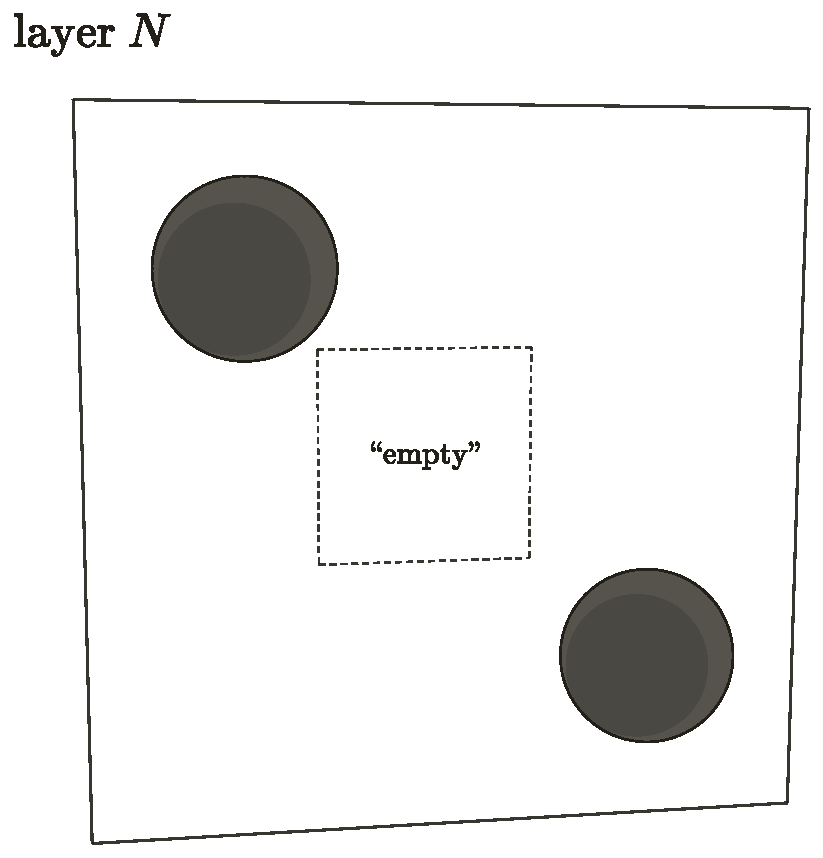
\includegraphics[width=0.48\textwidth]{figures/bbu_actorsbelow_bodies}\hfill
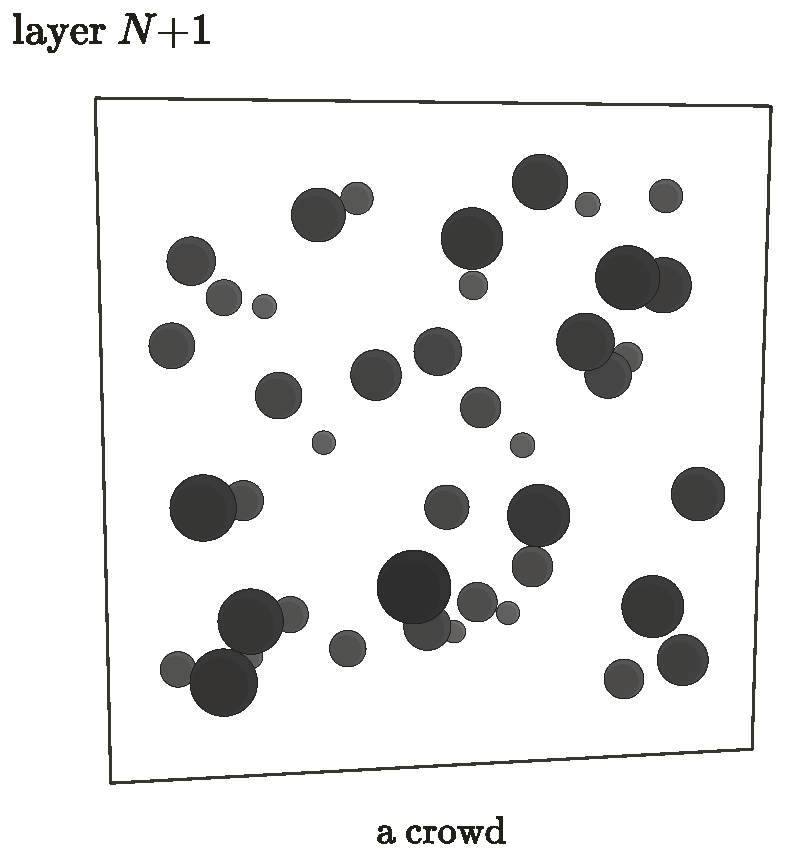
\includegraphics[width=0.48\textwidth]{figures/bbu_actorsbelow_crowd}
\caption{The first rule of the sketch: space is the actors below. The ``empty'' space of layer $N$ (left) --- the void through which its bodies supposedly act --- is, magnified, the crowd of layer $N{+}1$ (right). Their arrangement is our geometry; their motions are our physics of empty space; and their own space is another crowd, without end. Once the void is a crowd, ``empty space transmits forces'' stops being a mystery: transmission is just what crowds do.}
\label{fig:actorsbelow}
\end{figure}

Notice what this one rule buys. The book's two founding convictions --- no action at a distance, and no bottom --- stop being separate demands. Each requires the other. A mediated universe needs a medium; a medium made of actors needs its own space; that space needs actors below it; and so on, without end. The no-magic principle, applied to space, \emph{generates} the layers. The tower is not an extravagance bolted onto the mechanics. It is what the mechanics stand in.

And notice what it dissolves. ``Empty space transmits forces'' --- the phrase that has embarrassed physics since Newton --- stops being mysterious the moment ``empty space'' is a crowd. Of course the crowd can transmit: transmission is just the crowd doing what crowds of actors do --- colliding, streaming, pushing. The rest of this chapter is an inventory of what a crowd can do.

\section{Second Rule: No Action at a Distance --- and None at a Depth}

The first rule says what space is made of. The second says how anything in it is allowed to act, and since it is the rule this whole book grew out of, I will state it plainly and then be careful about how much of it I can show.

Nothing acts where it is not. A body influences its neighbours by touching them --- through the crowd between, by what arrives and what fails to arrive --- and never by reaching across a gap with nothing in the gap. That is Chapter~1's complaint, grown up. It is why gravity in this sketch is a push from what is there rather than a pull from what is not.

Now turn the same rule on its side. The tower has a vertical direction as well as a horizontal one, and the prohibition ought to hold in both. What happens in a layer is local to that layer and its neighbours: a body acts on the crowd immediately below it and is acted on by that crowd, and whatever happens three floors down reaches us only by being handed up, floor by floor, like buckets in a line. There is no channel from our layer to the depths that skips the floors between. No action at a distance --- and none at a depth either.

I want to be exact about the standing of these two halves, because they are not equally secured. The horizontal half is this book's founding conviction, and everything in the sketch obeys it. The vertical half is a \emph{conjecture}. I believe it firmly --- a tower whose floors could reach past one another would not be a tower but a heap --- and I cannot prove it, and I am not claiming that the alternative is impossible.

The rule earns its keep by what it buys. It makes the tower's endlessness harmless: no event involves infinitely many layers, because no event reaches past its neighbours, so there are no infinite sums anywhere in the physics --- only chains, each link finite. It explains why the tower is invisible from where we stand: we are in contact with one floor down, and everything deeper arrives filtered through everything between. And it settles the shape of the escape the next chapter's first wound will need, and gives it its name: the \emph{\Ix{cascade}} --- energy handed downward one layer at a time, each layer passing on what it cannot keep, none of them warming.


\section{Gravity: The Shadow Push}

So let there be a \Ix{flux}. Through every layer's space --- that is, through the crowd of the layer below --- small fast particles stream in all directions equally. Call them \emph{\Ix{massion}s}: the notes this book grew from coined the word, and I have kept it. From every direction, at every moment, everything is being peppered.

A lone object in this rain feels nothing net. Hit equally from all sides, it stays put --- the way a swimmer treading water in a perfectly uniform current from all directions goes nowhere. The flux is omnipresent and, alone, undetectable \emph{as a force} --- what else it might announce, heat above all, is Chapter~7's first war. This is important: in this sketch, you do not feel the sea you are in. You feel only its \emph{imbalances}.

Now place two objects near each other. Each absorbs, or scatters, some of the flux passing through it. So each casts a \emph{shadow} --- a thinning of the rain on its far side. And each object sits partly in the other's shadow. The rain still hammers them from every outward direction, but from the direction of the neighbour it arrives diminished. The imbalance pushes each toward the other.

That push is gravity. Not a pull --- nothing in this universe pulls; pulling-at-a-distance is the original cheat. What looks like mutual attraction is mutual \emph{sheltering}: two objects shielding each other from the universal rain and being pressed together by all the rain they don't shield. The picture in my oldest notes is two air bubbles rising in water, which drift together not because they desire each other but because the water between them is calmer. A story sailors are said to have told --- the historical record, I must add, is thinner than the story --- makes the same picture at human scale: two ships in a swell, side by side, drifting dangerously together~\cite{boersma1996}, each blocking the waves from the other while the unblocked waves outside do the rest. Whether or not any bosun ever logged it, the geometry of the picture is sound, and it is the geometry this book is borrowing --- the bookkeeping, Chapter~7 will insist, is another matter.

\begin{figure}[htbp]
\centering
% Figure authored as a proofviz sketch (proofs/bbu_shadowpush.sketch.js);
% regenerate with `node scripts/make-deliverables.mjs bbu_shadowpush`, copy
% the PDFs here and `pdfcrop --margins 6` each. The sketch machine-checks
% that the 'alone' rain directions sum to zero (no net force).
\begin{minipage}[t]{0.45\textwidth}\centering
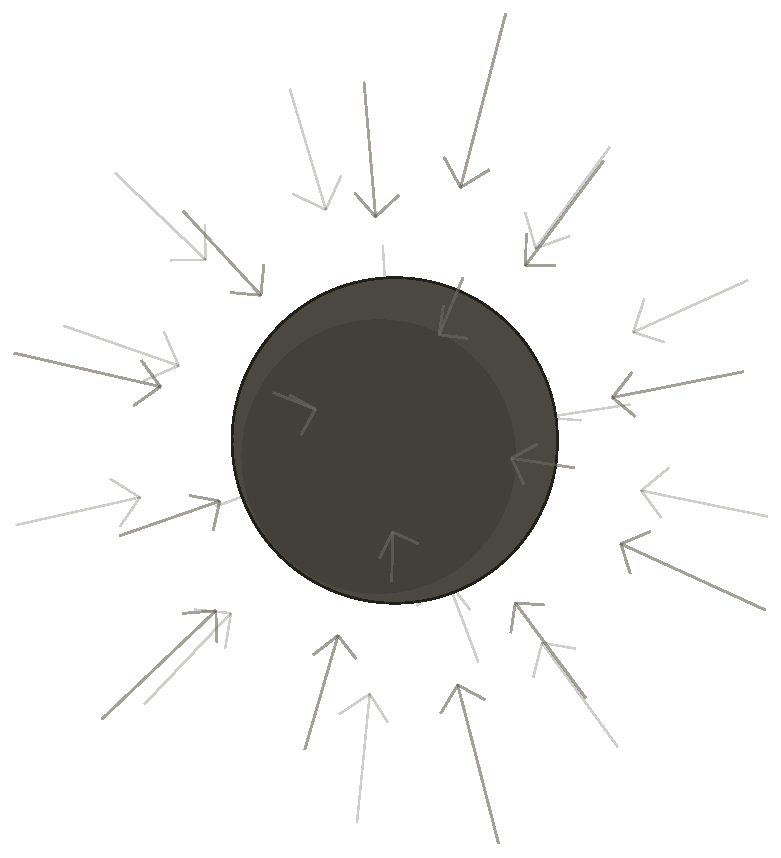
\includegraphics[width=\linewidth]{figures/bbu_shadowpush_alone}\\
{\small (a) alone: hit equally from all sides --- no net force}
\end{minipage}\hfill
\begin{minipage}[t]{0.51\textwidth}\centering
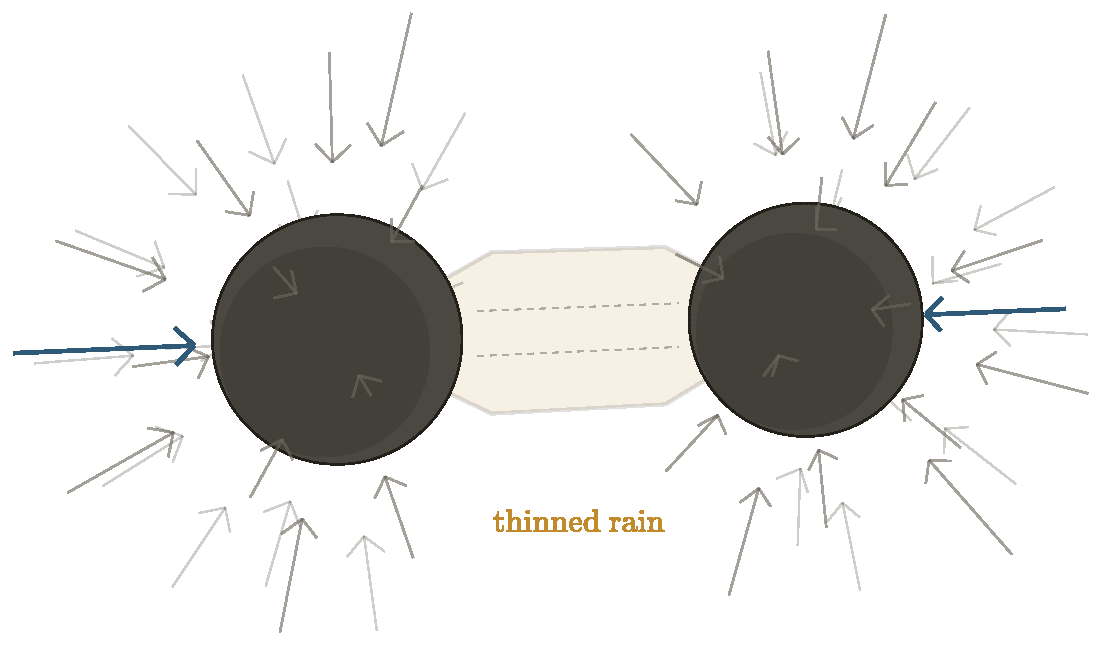
\includegraphics[width=\linewidth]{figures/bbu_shadowpush_together}\\
{\small (b) together: each shades the other --- the unshaded rain pushes them together}
\end{minipage}
\caption{The \Ix{shadow push}. (a)~A lone body in the universal rain of massions is struck equally from every direction: the flux is omnipresent and, alone, undetectable. (b)~Two bodies each absorb part of the flux passing through them, so each casts a shadow --- a thinning of the rain on its far side --- and each sits partly in the other's shadow. The rain still hammers them from every outward direction, but from the direction of the neighbour it arrives diminished (dashed). The imbalance (bold arrows) presses them together: not a pull, but mutual sheltering. Because the shadow a body casts covers an angle of its neighbour's sky, and angular size falls off as the square of the distance, the push inherits the inverse-square law from geometry itself.}
\label{fig:shadowpush}
\end{figure}

\begin{figure}[p]\centering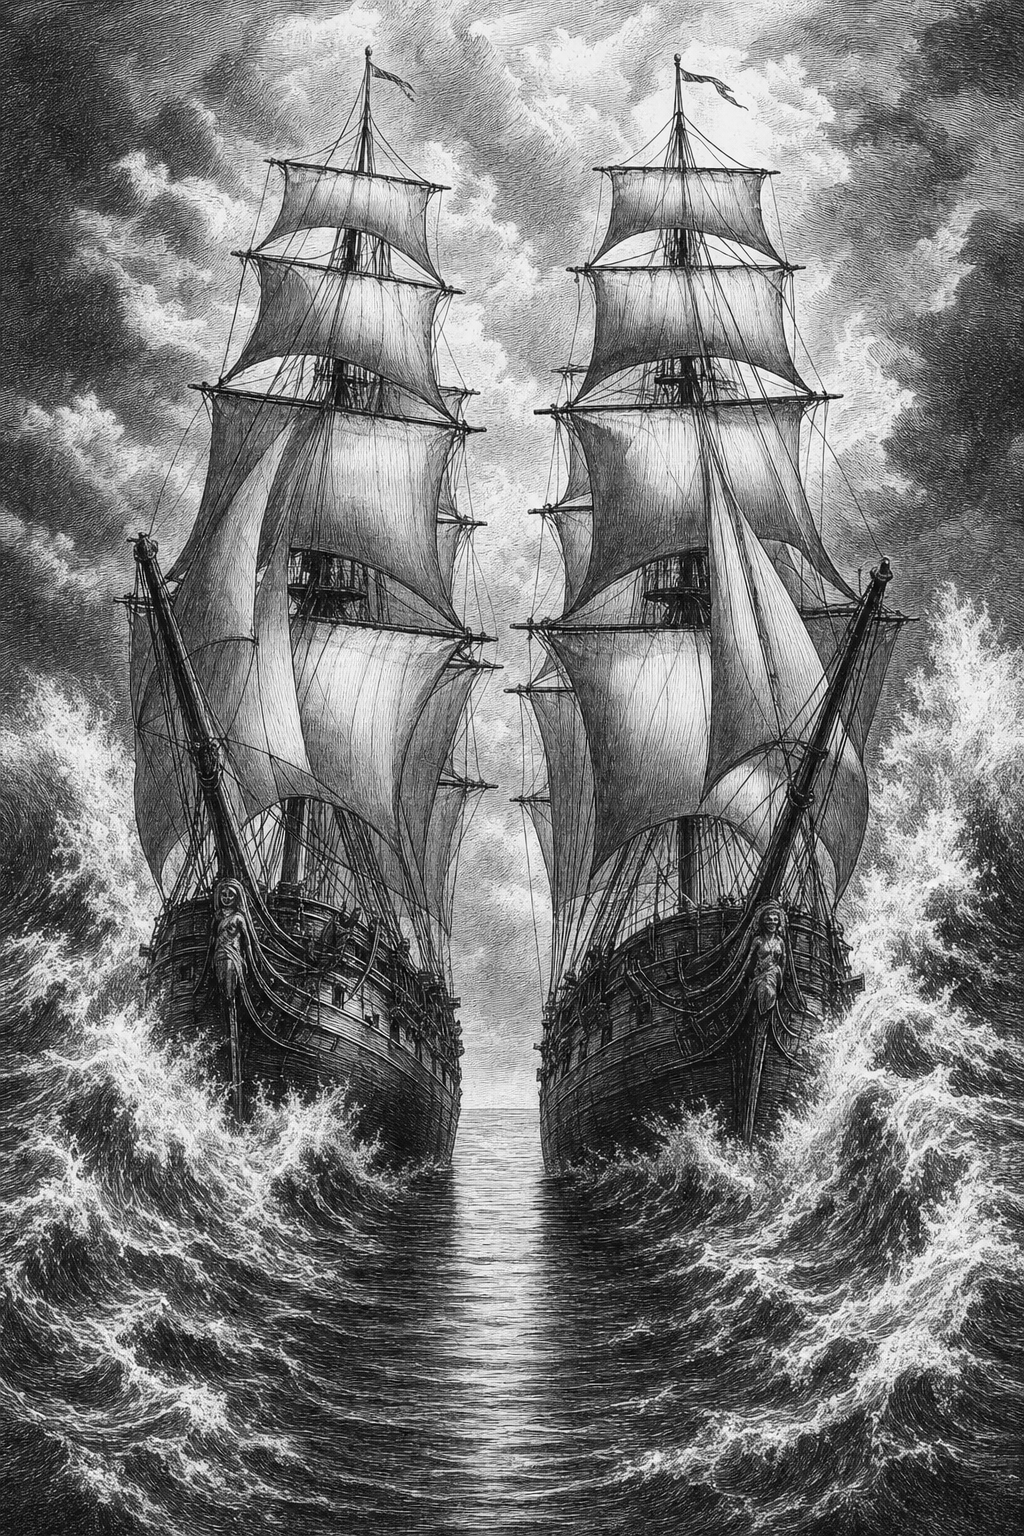
\includegraphics[height=0.92\textheight,width=\textwidth,keepaspectratio]{art/plate_two_ships}\end{figure}

The sketch even yields the right \emph{shape} of law, and this is worth pausing on. How much of your neighbour's shadow do you sit in? That depends on the angle it covers in your sky --- and the angular size of a shadow falls off as the square of the distance. Double the separation and the neighbour blocks a quarter of the directions it blocked before. An inverse-square law, not assumed, but \emph{inherited from geometry itself} --- from the mere fact that shadows shrink with distance in three-dimensional space.\footnote{Exactly, in the limit that the bodies are small compared to the distance between them --- a condition every orbit in this book satisfies with room to spare.} (Shadows must also stay \emph{thin} --- each body dimming the rain so slightly that two shadows simply add; whether nature honours that, and where it might stop, is the sixth wound's whole business.) Newton's exponent, the sacred 2, stops being a decree and becomes a consequence: it is the dimensionality of the crowd, showing through. (And a reader of Tegmark's argument, quoted in this book's earliest notes, will see the same fact from the other side: in four spatial dimensions, shadow-geometry would give an inverse-cube law --- under which no orbit is stable~\cite{ehrenfest1917}. A universe of shadow-gravity that contains observers watching stable orbits will be a universe of three-dimensional crowds. The sketch does not just permit our dimensionality; it is most at home in it.)


% Figure authored as a proofviz sketch (proofs/bbu_inverse_square.sketch.js);
% regenerate with `node scripts/make-deliverables.mjs bbu_inverse_square`,
% copy the PDFs from exports/bbu_inverse_square/ into figures/, then
% `pdfcrop --margins 6 <f>.pdf <f>.pdf` each (the export canvas has margins).
% The sketch carries machine checks: tangency, α(2d)≈α(d)/2, blocked solid
% angle at 2d ≈ 1/4 (exact as ρ/d→0).
\begin{figure}[htbp]
\centering
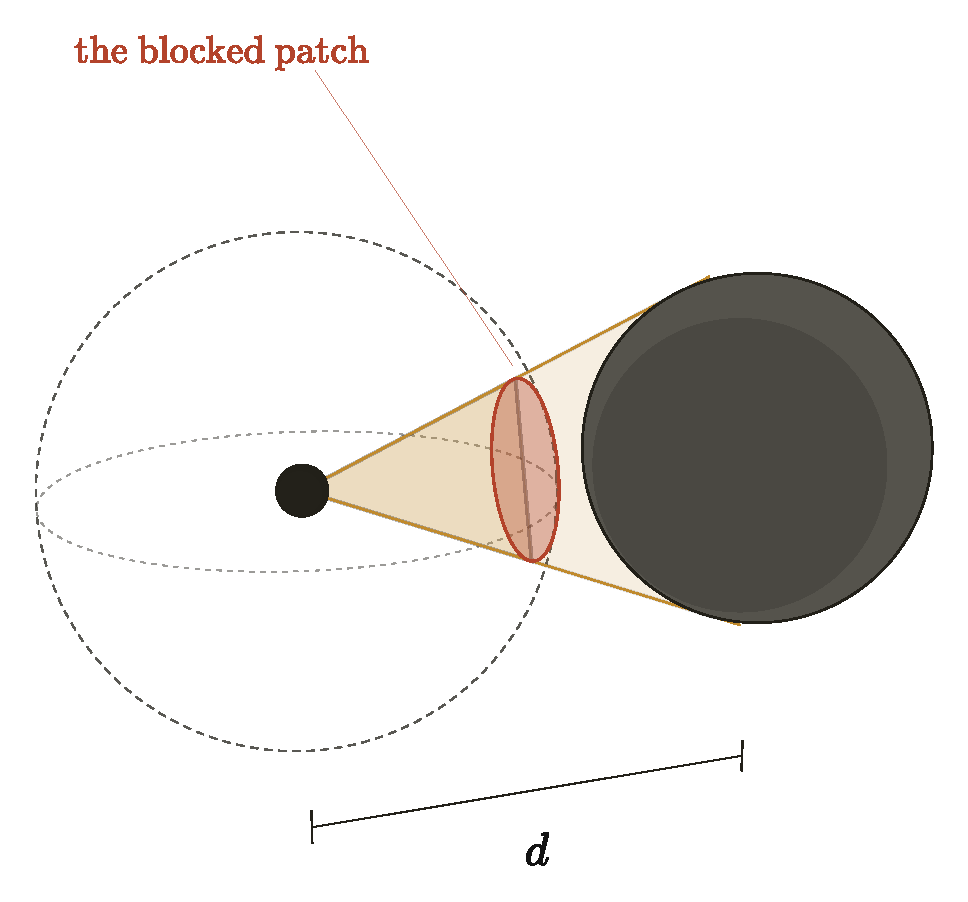
\includegraphics[width=0.75\textwidth]{figures/bbu_inverse_square_near}\\[0.4em]
{\small at distance $d$: the neighbour blocks the red patch of the sky --- the sphere of directions the rain arrives from}\\[0.7em]
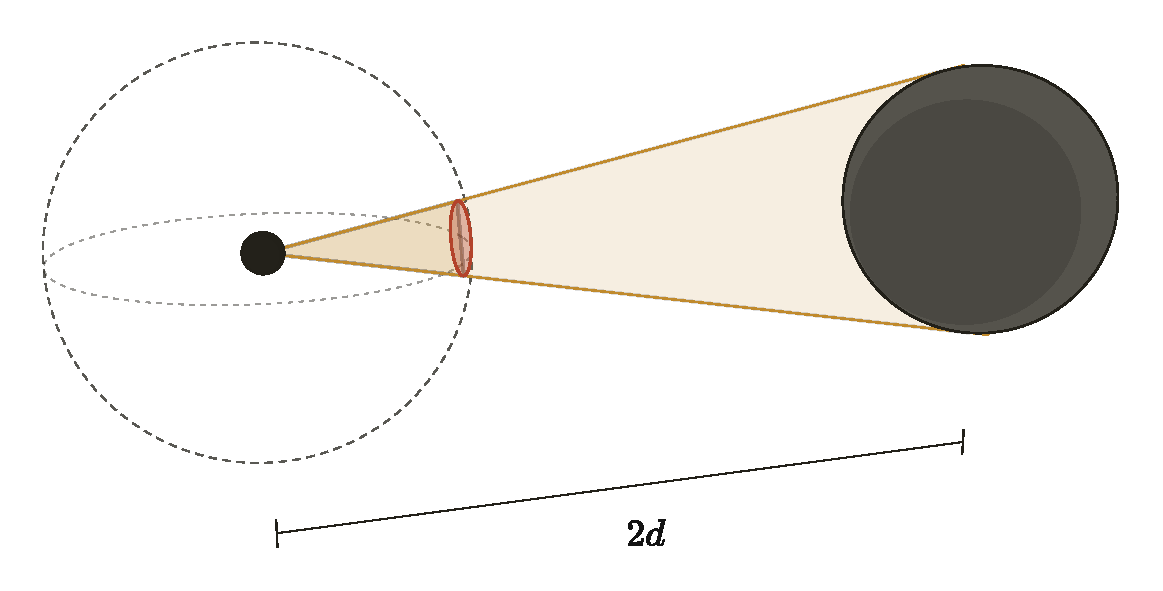
\includegraphics[width=0.78\textwidth]{figures/bbu_inverse_square_far}\\[0.4em]
{\small at distance $2d$: half the angular width --- one quarter of the sky directions}
\caption{Newton's exponent, inherited from geometry. How hard the shadow push acts on a body depends on how much of its sky the neighbour blocks. Double the separation and the neighbour's angular width halves, so the blocked patch of sky --- an area on the sphere of directions --- shrinks to one quarter. The imbalance in the rain, and with it the push, falls off as the square of the distance: not a decree, but the dimensionality of the crowd showing through. (In four spatial dimensions the same geometry would give an inverse cube, under which no orbit is stable.)}
\label{fig:inversesquare}
\end{figure}

\section{Charge: Orbits and Orientation}

Gravity, in this sketch, is about \emph{blocking}. Charge is about \emph{circulation}.

Let some particles be orbited by others --- a central mote with companions wheeling around it in a plane, the whole assembly emitting and receiving smaller particles of its own. Now two such assemblies can differ in two purely geometric ways: the \emph{orientation} of the orbital plane, and the \emph{sense} of the circulation --- clockwise or anticlockwise, seen from a given side.

The old notes propose: this geometry \emph{is} charge. A ``positive'' object is such an assembly circulating one way; a ``negative'' object is the mirror arrangement. And the interactions follow from collisions of circulation, not from any charge-stuff:

Two assemblies circulating the \emph{same} way, meeting, clash --- their streams meet head-on where the assemblies face each other, pile up, and press the assemblies apart. Like repels like, not by decree, but the way two water-vortices spinning the same sense shoulder each other away.

Two assemblies circulating \emph{opposite} ways interlock --- their streams at the meeting face run together, cancel, quiet the space between them. Each now shelters the other from the general agitation, and the shadow-push does the rest: unlike charges attract by the same mechanism as gravity, only fiercer, because circulation-cancellation quiets the space far more thoroughly than mere blocking thins it.

And an invoice arrives with the pair of mechanisms, which I book now and the wounds table will carry: pushing-apart by pile-up and pressing-together by quiet are \emph{different} mechanisms, and nothing in the sketch says their strengths must match --- yet measured attraction and repulsion between equal charges agree to better than a part in a thousand million million million. Two mechanisms, one magnitude, no derivation: filed~\cite{bressi2011}.

And orientation gives a third possibility that plain gravity lacks: two orbital planes at right angles to each other simply \emph{miss}. Their circulations neither pile nor cancel; they thread through one another's business without transacting, the way two polarizing filters\footnote{A polarizing filter passes only light whose sideways vibration lies along one axis; cross two at right angles and nothing gets through --- sunglasses and camera filters do it daily. (Dictionary: polarization.)} at ninety degrees pass no common light. In this sketch, that is what it is for two things to not interact: not a permission withheld, but a geometry that never meets.


\begin{figure}[htbp]
\centering
% Figure authored as a proofviz sketch (proofs/bbu_circulation.sketch.js);
% regenerate with `node scripts/make-deliverables.mjs bbu_circulation`, copy
% the PDFs here and `pdfcrop --margins 6` each. The sketch machine-checks
% that the two ring planes in (iii) are orthogonal (n1*n2 = 0).
\begin{minipage}[t]{0.32\textwidth}\centering
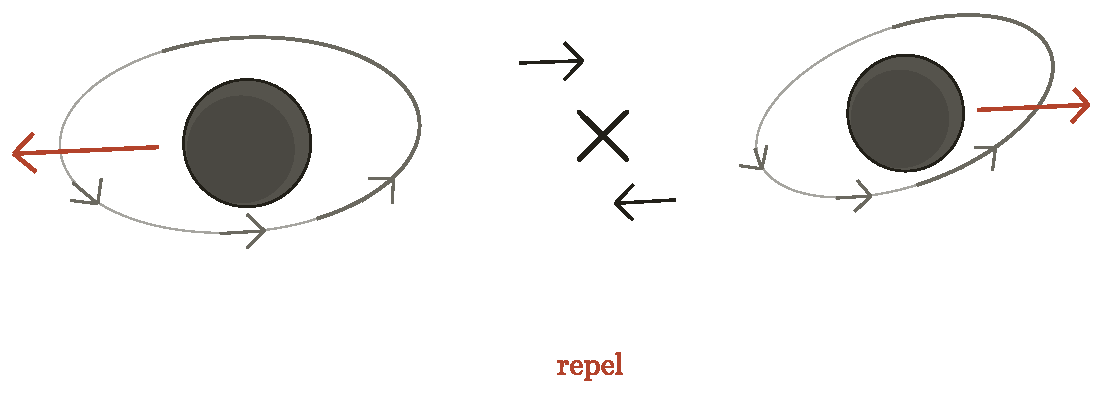
\includegraphics[width=\linewidth]{figures/bbu_circulation_same}\\
{\small (i) same sense: streams meet head-on --- pile up, repel}
\end{minipage}\hfill
\begin{minipage}[t]{0.32\textwidth}\centering
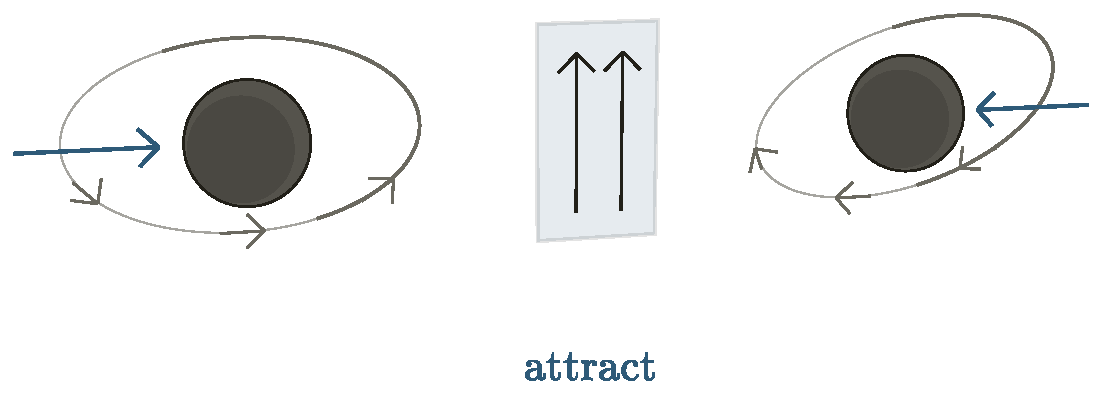
\includegraphics[width=\linewidth]{figures/bbu_circulation_opposite}\\
{\small (ii) opposite sense: streams run together and cancel --- quiet space, attract}
\end{minipage}\hfill
\begin{minipage}[t]{0.32\textwidth}\centering
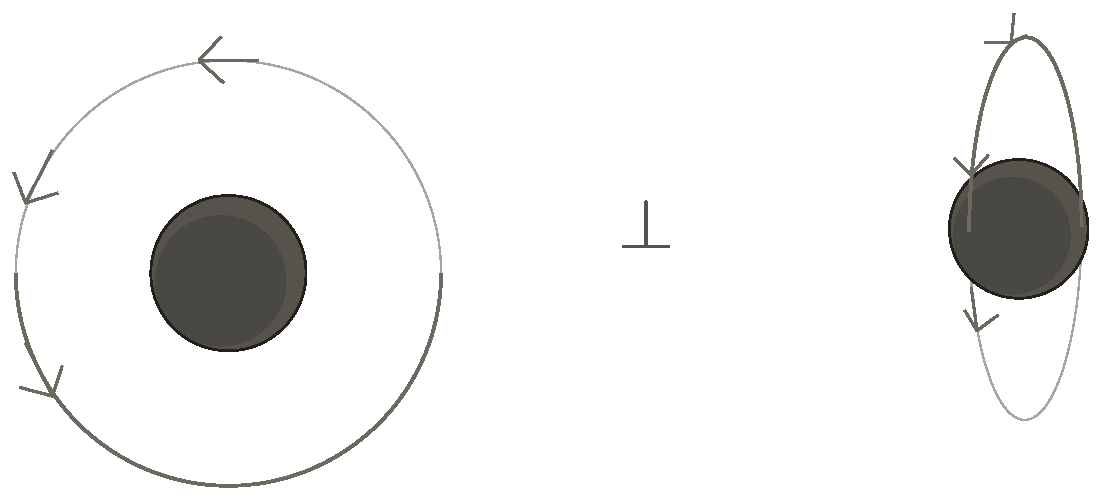
\includegraphics[width=\linewidth]{figures/bbu_circulation_ortho}\\
{\small (iii) orthogonal planes: the circulations thread past --- no interaction}
\end{minipage}
\caption{Charge as circulation. Each charged assembly sheds circulating streams of its own substance. (i)~Two assemblies circulating the \emph{same} sense present head-on streams where they face each other: the streams pile up and the assemblies are pressed apart --- like repels like. (ii)~\emph{Opposite} senses present aligned streams: they cancel, quiet the space between (shaded), and the shadow push does the rest --- opposites attract, by the same mechanism as gravity but fiercer. (iii)~Orbital planes at right angles neither pile nor cancel: the circulations pass through one another's business without transacting, as two crossed polarizing filters pass no common light.}
\label{fig:circulation}
\end{figure}

Push the same move one layer down and even the strange three-fingered rules of electromagnetism --- force at right angles to both motion and field, the rule every physics student memorizes with a contorted hand --- stop looking arbitrary. Where circulations meet circulations, the resultant push is perpendicular to both by the plain geometry of colliding streams. \Iyk{Orsted}{\O rsted}'s compass needle, twitching beside its wire in Copenhagen, was the first sight of exactly this --- force running in circles about a current --- and Chapter~2 called that swirl the lineage's one experimental gift to this chapter. This paragraph is where the gift is spent. I do not claim the sketch derives Maxwell's equations; it does not, and Chapter 7 will be blunt about the gap. I claim the \emph{kind} of thing electromagnetism is --- directional, chiral, orthogonality-respecting --- is the kind of thing circulating crowds naturally produce, and that this is more than coincidence deserves.

Annihilation, too, falls out rather than being added. Two assemblies of opposite circulation that do not merely meet but \emph{collide} --- centre into centre --- have their orbits run head-on into each other's orbits. Counter-circulating streams at full interpenetration do not shelter; they cancel \emph{catastrophically}, each unwinding the other's circulation entirely. What remains is no longer two charged assemblies but the energy of their unwound circulations, dumped into the crowd at a stroke --- and a disturbance dumped into a crowd departs as the crowd's own waves, a claim this chapter will make in earnest a few pages from now. A positive and a negative object, meeting exactly, cease to be objects and leave as radiation --- two equal flashes of light, back to back --- which is what matter and antimatter have been observed to do since 1932.\footnote{1932: Carl Anderson's discovery of the positron, the electron's opposite twin; the mutual destruction of matter and antimatter followed into the textbooks.}

\section{States of the Crowd: Frozen and Gas}

A crowd of orbiting assemblies has collective conditions, the way water does. Call a region \emph{gas} when its assemblies wander freely, all agitation and passage. Call it \emph{frozen} when the circulations of neighbouring assemblies have locked --- opposite-sense neighbours interlocked in the quiet-space embrace described above --- into a structure that holds its shape.

Two consequences from the old notes, both of which I still find striking:

First: \textbf{two frozen objects in a gas drift together.} Between them, each \emph{absorbs} part of the other's agitation --- soaks it into its interlocked circulations, the same capacity that sets its melting point below --- and what is soaked up is not returned: the gas between them runs quieter than the gas outside; the outside wins. (Absorption is doing the work in that sentence. Chapter~7 will show that elastic blocking --- catching and returning --- buys no push at all; the drift is real only because a frozen thing \emph{keeps} part of what it catches.) This is the shadow-push again, appearing at a new scale, unbidden --- the sketch's mechanisms repeat across levels without being re-installed, which is exactly what a layered universe ought to do. And two frozen objects pressed by a surrounding gas, if they are also moving, do not merely collide: they can fall into orbit around one another --- though capture, the reader should note, needs something to carry surplus motion away, and here that something is the same absorption already doing the pushing.

Second: \textbf{a frozen thing can melt.} A structure held by interlocked circulations holds only up to a certain agitation. Heat the crowd enough --- agitate the assemblies past what the interlocking can absorb --- and the structure lets go. The old notes put it in one sentence I have never improved on: \emph{a proton is perhaps frozen, and decays --- melts --- when it becomes hot enough.} (The laboratory has since met something with this shape: hot enough, protons and neutrons do dissolve --- the quark--gluon plasma\footnote{A plasma is a gas so hot its atoms have come apart into charged fragments --- the state of matter of stars, flames, and lightning.} of the collider experiments --- though the standard account calls that deconfinement, not decay, and the proton alone, in the cold, has never once been seen to die.) Stability is not a permission granted to certain particles and denied to others; it is a phase, like ice. Matter persists because its region of the crowd is cold; push any matter into a hot enough region and it returns to gas. That the early universe --- hot beyond all measure --- should have been a place where no structure could freeze, and that matter as we know it should have condensed out as things cooled: in this sketch, that is not a special story requiring its own physics. It is what happens to any pond in autumn.


\begin{figure}[htbp]
\centering
\begin{tikzpicture}[>=stealth]
  % ------- (i) gas -------
  \begin{scope}[xshift=0.1cm]
    \foreach \p/\s in {(0.5,2.6)/1,(1.7,2.9)/-1,(2.6,2.3)/1,(0.9,1.7)/-1,(2.1,1.5)/1,(0.45,0.7)/1,(1.5,0.5)/-1,(2.7,0.8)/-1} {
      \draw[black!60, ->] \p ++(30:0.24) arc[start angle=30, end angle=300, radius=0.24];
    }
    \node[anchor=north, align=center, text width=3.0cm] at (1.6,-0.15)
      {\small (i) gas: assemblies\\ wander freely};
  \end{scope}
  % ------- (ii) frozen -------
  \begin{scope}[xshift=4.05cm]
    \foreach \i in {0,1,2} \foreach \j in {0,1,2} {
      % opposite senses on the two sublattices, told apart by shade as well as
      % arrowhead (the heads alone are too subtle at this size)
      \pgfmathparse{mod(\i+\j,2)==0 ? 1 : 0}
      \ifnum\pgfmathresult>0
        \draw[black!70, ->] ({0.55+\i*1.05},{0.55+\j*1.05}) ++(30:0.26) arc[start angle=30, end angle=310, radius=0.26];
      \else
        \draw[bbuBlue!80, <-] ({0.55+\i*1.05},{0.55+\j*1.05}) ++(30:0.26) arc[start angle=30, end angle=310, radius=0.26];
      \fi
    }
    % bonds
    \foreach \i in {0,1} \foreach \j in {0,1,2} {
      \draw[black!25] ({0.55+\i*1.05+0.28},{0.55+\j*1.05}) -- ({0.55+\i*1.05+0.77},{0.55+\j*1.05});
      \draw[black!25] ({0.55+\j*1.05},{0.55+\i*1.05+0.28}) -- ({0.55+\j*1.05},{0.55+\i*1.05+0.77});
    }
    \node[anchor=north, align=center, text width=3.0cm] at (1.6,-0.15)
      {\small (ii) frozen: opposite senses\\ interlock into structure};
  \end{scope}
  % ------- (iii) two frozen bodies in gas -------
  \begin{scope}[xshift=8.0cm]
    % gas dots, denser outside than between
    \foreach \p in {(0.25,2.9),(0.9,3.1),(1.9,3.05),(2.7,2.85),(3.1,2.2),(0.2,2.1),(0.35,1.2),(0.2,0.4),(0.9,0.25),(1.8,0.2),(2.6,0.35),(3.15,0.9),(3.05,1.6),(1.35,2.75),(2.35,0.6)}
      \fill[black!50] \p circle (0.06);
    \fill[bbuGold!25] (1.25,1.05) rectangle (2.15,1.95); % quiet corridor between
    \draw[fill=black!35] (0.55,1.15) rectangle (1.25,1.85);
    \draw[fill=black!35] (2.15,1.15) rectangle (2.85,1.85);
    \draw[->, bbuBlue, line width=1.4pt] (0.12,1.5) -- (0.57,1.5);
    \draw[->, bbuBlue, line width=1.4pt] (3.28,1.5) -- (2.83,1.5);
    \node[anchor=north, align=center, text width=3.0cm] at (1.7,-0.15)
      {\small (iii) two frozen bodies\\ in a gas drift together};
  \end{scope}
\end{tikzpicture}
\caption{States of the crowd. (i)~Gas: assemblies wander, all agitation and passage. (ii)~Frozen: neighbouring circulations of opposite sense interlock into a structure that holds its shape --- matter as local winter; heat the crowd past what the interlocking can absorb and the structure lets go, which is what decay is. (iii)~Two frozen bodies in a gas shelter each other: the agitation between them (shaded) is calmer than the agitation outside, and the outside wins --- the shadow push reappearing at a new scale, unbidden.}
\label{fig:frozengas}
\end{figure}

Even the charged objects themselves, the notes suggest, are frozen things --- but imperfectly frozen: they \emph{sublimate}, shedding small circulating pieces of themselves in all directions, the way ice smokes in dry winter air. That shed circulation is the ``field'' around a charge --- not a field at all, but weather: the object's own substance, departing, carrying its circulation-sense outward to interlock or collide with whatever it meets.

\section{Light}

What, then, is light? The old notes give one line: \emph{light is an object orbited by another, in motion --- a wave.} I will unfold it first exactly as written --- and then, because writing this book taught me where it fails, rebuild it into something stronger out of this chapter's own parts.

Take the smallest assembly there is at a given layer --- one mote and one companion, wheeling. Set the pair moving through the crowd. What passes any fixed point is a \emph{circulation arriving periodically}: the companion swings near, swings far, near, far, as the pair travels --- a regular beat of push delivered to everything along the path. A travelling circulation is a travelling oscillation. It has a frequency: the wheeling rate. It has an orientation: the plane of the orbit --- and there is polarization, not as an extra property bolted on, but as the geometry the object could not help having. Turn two such travellers' planes perpendicular and they transact nothing with each other, and interact differently with everything else --- the polarizing filter again, now as optics.

And the oldest of all the questions about light --- is it a particle or a wave? --- receives, in the sketch, the mildest possible answer: it is a particle \emph{doing} a wave. The travelling pair is as localized as any particle, and delivers its pushes in discrete arrivals; the pattern of those arrivals along the path is as periodic as any wave. The sketch does not pretend this settles a century of quantum mechanics. But it is worth noticing that the toy's most economical object --- two motes and a motion --- arrives already wearing both costumes.


\begin{figure}[htbp]
\centering
% Figure authored as a proofviz sketch (proofs/bbu_lightpair.sketch.js);
% regenerate with `node scripts/make-deliverables.mjs bbu_lightpair`, copy
% the PDFs here and `pdfcrop --margins 6` each. The sketch machine-checks
% constant orbit radius and axial advance per turn = lambda.
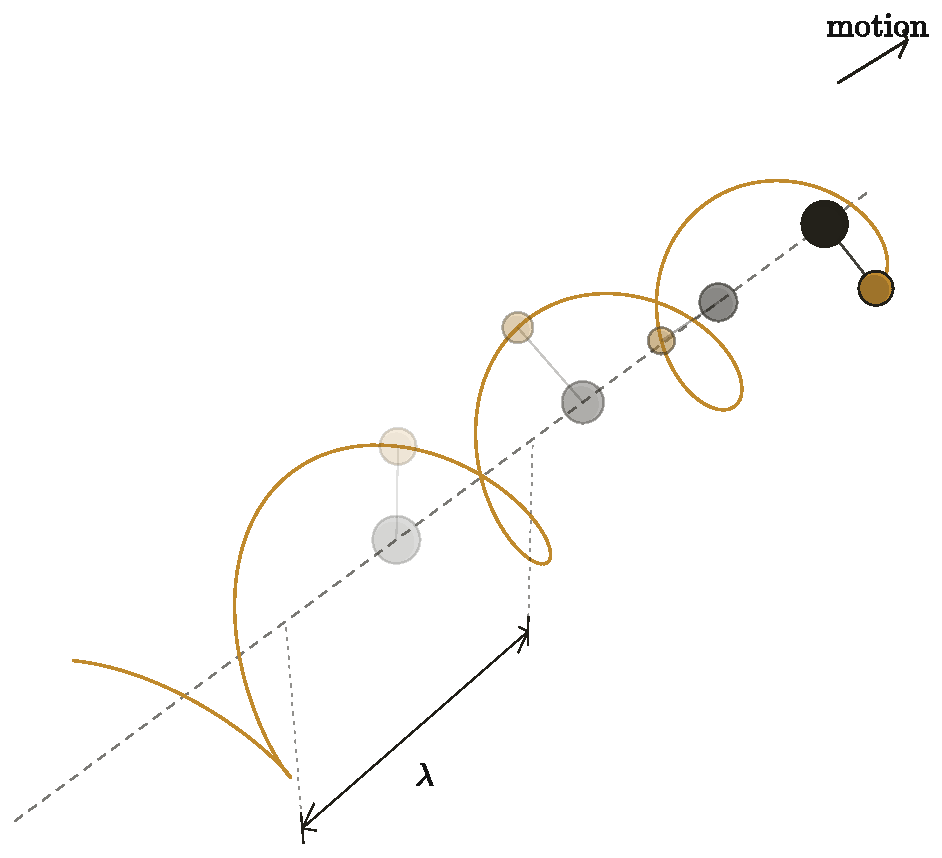
\includegraphics[width=0.57\textwidth]{figures/bbu_lightpair_travel}\\[0.2em]
\parbox{0.9\textwidth}{\centering\small the smallest assembly --- one mote, one wheeling companion --- set moving: what passes any fixed point is a circulation arriving periodically}\\[0.6em]
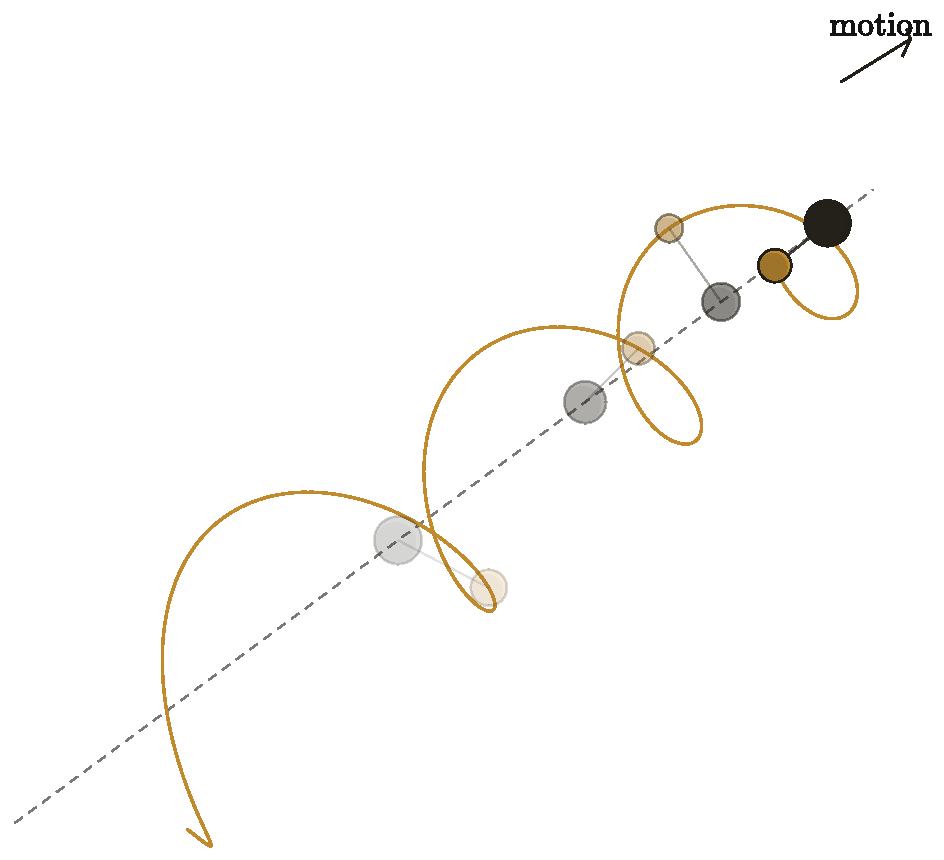
\includegraphics[width=0.57\textwidth]{figures/bbu_lightpair_pol}\\[0.2em]
{\small the same traveller, plane turned $90^{\circ}$: polarization}
\caption{The first sketch of light: an object orbited by another, in motion --- a particle doing a wave. The travelling pair is as localized as any particle and delivers its pushes in discrete arrivals; the pattern of those arrivals along the path is as periodic as any wave, with a frequency (the wheeling rate) and an orientation (the plane of the orbit). Turn the plane ninety degrees (right) and you have the other polarization --- not a property bolted on, but geometry the object could not help having. The section keeps this picture --- demoted: as the portrait of a localized wave-packet of the medium, not the traveller itself.}
\label{fig:lightpair}
\end{figure}

That was the sketch as my notes first drew it, and I have kept it because it earns its keep --- but writing this book has taught me its two failures, and they are not small ones. First: \emph{universal} $c$. Every pair, whatever its wheeling rate, whatever its history, moves at exactly the same speed --- the same to one part in a thousand million million, dispersionless across a billion years of travel. Nothing about a composite assembly explains that; assemblies should vary. Second: interference. A lone travelling pair does not bend around corners, and it cannot cancel itself into the dark bands of the two-slit pattern; those are things \emph{waves in a medium} do, and no solitary traveller does them. Light's two most famous behaviours, and the pair can do neither.

But this chapter has already built, for other reasons, exactly the thing that can. The First Rule made the vacuum a crowd. The \Ix{frozen state} made a crowd that holds its shape --- interlocked circulations, a structure with tension in it. And a structured medium with tension \emph{sings}: it carries transverse waves of its own substance, at a speed set not by the wave's history but by the medium --- one crowd, one wave speed, for every frequency, from every source, the way sound in air does not care who shouted. So here is the upgrade, and I state it as a replacement of mechanism, not of image: \emph{light is not a traveller through the vacuum-crowd; light is the vacuum-crowd's own song.} A transverse wave \emph{of} the medium. At one stroke the two failures --- universal $c$ and interference --- dissolve: universal $c$ is a medium property --- one speed in the \emph{medium's} frame, which is not yet the stranger fact that every moving observer measures the same speed; that bill is presented, and paid at conspiracy prices, in the second wound --- dispersionlessness is the medium's linearity, and interference, diffraction, the dark bands --- these are what medium-waves do natively, no purchase required. Refraction arrives free: light slows in glass because glass is a denser, mixed crowd. The wave was never the hard part. The hard part was always the lump.

And the lump is bought with a coin this chapter has been minting for pages without naming. Name it now: the \emph{\Ix{gap}} --- the fact that a bound quantum system has a lowest step, and below that step it cannot absorb at all; energy is taken in lumps or not taken. A \emph{quantized} medium's waves come in lumps --- granting the quantization, a grant this chapter's closing honesty will price --- condensed-matter physics has a name for exactly this, the \Ix{phonon},\footnote{The phonon: the quantum of sound in a crystal --- vibration of a lattice, which quantum mechanics obliges to come in discrete lumps. Proof by existence that a medium's waves can be particles. (Dictionary.)} the particle of a crystal's sound --- and the \Ix{photon}, in this picture, is the vacuum-crowd's transverse phonon: the smallest lump of the medium's song that the gap permits. The travelling pair of the figure is not discarded; it is demoted and preserved. It is the \emph{portrait} of a wave-packet --- what a localized lump of the medium's wave looks like when you squint: compact, periodic, arriving in discrete pushes, carrying its plane. The sketch had the right picture and the wrong ontology: wave-first, with the particle emergent, is the right way round --- and it is, for what it is worth, the way the twentieth century's own field theory rounds it too.

And I owe the reader a structural honesty before the figure below, because the chapter has now asked the crowd to be two things. The rain of the opening --- fast, free, streaming through everything --- and the frozen lattice of this section --- interlocked, tense, singing --- are not one population wearing two hats; they are two populations of the same layer, coexisting in the same space: a lattice threaded by a wind. That is not incoherent --- a star is exactly such a place, its plasma carrying sound while neutrinos stream through the same volume barely touching it --- but it is a real structural commitment, and the next chapter's accounting must serve both tenants at once: the rain passing through the lattice as freely as gravity's transparency demands, the lattice holding the tension light's stiffness demands. One crowd, two phases, and the books of both must balance.

\begin{figure}[htbp]
\centering
\begin{tikzpicture}[>=stealth]
  % ---- (a) gravity: the crowd's push (streaming rain, shadow) ----
  \begin{scope}[xshift=-2.95cm]
    \foreach \p/\a in {(-1.9,1.55)/-40,(-1.2,1.8)/-75,(-0.3,1.7)/-100,(0.6,1.85)/-120,(1.5,1.6)/-140,(-2.0,0.0)/-15,(1.95,0.25)/195,(-1.85,-1.35)/35,(-0.9,-1.7)/70,(0.1,-1.8)/95,(1.1,-1.65)/115,(1.9,-1.3)/150}
      \draw[->, black!45] \p -- +(\a:0.55);
    \fill[bbuGold!25] (-0.62,-0.17) rectangle (0.62,0.17);
    \shade[ball color=black!65] (-0.85,0) circle (0.26);
    \shade[ball color=black!65] (0.85,0) circle (0.26);
    \draw[->, bbuBlue, line width=1.2pt] (-1.5,0) -- (-1.18,0);
    \draw[->, bbuBlue, line width=1.2pt] (1.5,0) -- (1.18,0);
    \node[anchor=north, align=center, text width=4.5cm] at (0,-2.1)
      {\small (a) gravity: the crowd's \emph{push} ---\\ streaming rain, and its imbalance};
  \end{scope}
  % ---- (b) light: the crowd's song (frozen lattice, transverse packet) ----
  \begin{scope}[xshift=2.95cm]
    % lattice rows with a transverse wave-packet
    \foreach \r in {-0.55,0,0.55} {
      \foreach \i in {0,...,16} {
        \pgfmathsetmacro{\x}{-2.0+\i*0.25}
        \pgfmathsetmacro{\env}{exp(-((\x)*(\x))/0.9)}
        \pgfmathsetmacro{\dy}{0.42*\env*sin(\i*80)}
        \fill[black!60] (\x,{\r+\dy}) circle (0.045);
      }
    }
    % envelope hint
    \draw[bbuGold, dashed, domain=-2.0:2.0, smooth, samples=50]
      plot (\x,{0.55+0.42*exp(-\x*\x/0.9)});
    \draw[bbuGold, dashed, domain=-2.0:2.0, smooth, samples=50]
      plot (\x,{-0.55-0.42*exp(-\x*\x/0.9)});
    \draw[->, line width=1.0pt] (1.15,1.35) -- (1.85,1.35);
    \node[anchor=south] at (1.5,1.4) {\small travels};
    \node[anchor=north, align=center, text width=4.5cm] at (0,-2.1)
      {\small (b) light: the crowd's \emph{song} ---\\ the frozen lattice itself waving; the lump is the photon};
  \end{scope}
\end{tikzpicture}
\caption{The rain and the song --- the same crowd, doing its two things. (a)~Gravity is what the crowd's \emph{streaming} does: an omnidirectional rain, and bodies pushed by nothing but its imbalance --- the shadow mechanism of this chapter's opening. (b)~Light is what the crowd's \emph{structure} does: the frozen, circulation-strung lattice waving transversely across the line of travel, the disturbance confined to a lump (dashed envelope) --- a wave-packet, the photon. One medium; a push and a song; and the difference between the two is the difference between weather and music.}
\label{fig:rainandsong}
\end{figure}

Charge then closes a loop I did not plan. Charge, in this chapter, is circulation; and a circulation \emph{shaken} --- an assembly accelerated --- cannot help disturbing the lattice it is embedded in: it sheds medium-waves. That is precisely what electromagnetism reports --- accelerated charges radiate --- now with a mechanism under it. And absorption runs the film backward: a resonant circulation catches a passing wave whole, or not at all, because the gap forbids partial purchase --- and there, in one sentence, is the all-or-nothing half of the photoelectric effect that began the quantum century~\cite{einstein1905photo}. Half, I said: the effect's other half is that the lump's energy climbs in exact step with the light's frequency, and that measured slope the sketch does not deliver. It is owed, not paid. One more consequence, and it is the one this book was always going to reach: our light is a wave of \emph{our} vacuum --- the crowd one layer down. But that crowd's own inhabitants have their own vacuum, the crowd below \emph{them}, with its own tension and its own transverse song --- faster than ours, if the layers quicken downward. \emph{Every layer has its own light, and its own} $c$. The speed of light is the loudest constant of our layer, not of the world: locally special, not globally special, now said of $c$ itself. What that buys, and what it costs, is Chapter~7's business.

\section{Why Things Are Alike}

One question remains that any mechanical universe must answer, because it is the question mechanics is worst at: why are things \emph{identical}? Every electron matches every other, everywhere, exactly. A universe of crowds and collisions ought, one would think, to produce endless slop --- assemblies of every size, orbits of every radius, a smear of almost-electrons. It produces instead a crisp catalogue of a few exact species. Why?

The old notes offer two answers --- one answer, I have come to think, seen from two sides --- and the writing of this book has forced a third.

The first: identical things are identical because they are \emph{made the same way} --- shed, as the sublimation picture has it, by parents that are themselves identical, the way every snowflake's sixfold symmetry is inherited from the one geometry of the water molecule. Identity propagates: like begets like, and the catalogue is a genealogy.

The second: the crowd itself may permit only certain assemblies to persist. Circulations interlock stably only at particular relations of size, speed, and spacing --- the way a plucked string, whatever you do to it, sounds only its own discrete harmonics, because only whole numbers of half-waves fit between its ends. Every other vibration dies at once; the survivors are exact, and exactly repeatable, not because anyone tuned them but because \emph{fitting} is an all-or-nothing affair. On this view the electron is not a thing that happens to be common; it is a \emph{resonance of the crowd} --- one of the few closed circulations that does not immediately unwind --- and it is identical everywhere for the same reason the third harmonic of every equal string is identical: the arithmetic of fitting has no almost.

And the third answer runs \emph{upward} through the layers, and it is a selection. Take the sketch's basic object --- a mote with a companion wheeling around it --- and ask what it needs in order to \emph{last}: to hold its orbit long enough for anything to be built from it. It needs the rain from below to be steady. Uniform in time, and uniform across the great distances the assembly will roam --- because a patchy crowd below means a varying push, and a varying push means orbits that drift, structures that shake themselves apart, nothing that accumulates. So long-lived structure at any layer \emph{certifies} the sameness of the layer beneath it, over exactly the reach and the ages that the structure has survived. Turn the certificate around and it becomes an explanation: things are alike down there wherever things persist up here --- not because unlikeness is impossible, but because unlikeness is \emph{uninhabitable}. Regions sitting over a motley crowd host no lasting assemblies, no chemistry, no memory, no one to ask why things are alike. We find identical electrons for the same kind of reason we find ourselves on a planet with water: the places without are not places where finding happens. My earliest notes contained this in embryo without my seeing it --- ``an expansion factor that limits the possibilities; otherwise, it disappears.'' \emph{Otherwise it disappears} is a selection principle. This is its grown form.

The three answers are not rivals; they stack, each carrying the part the others cannot. Selection explains the \emph{demand} --- a substrate must be uniform or bear nothing --- but selection's tolerance is loose: orbits forgive perturbations of a percent, while electrons match to twelve decimals, an overshoot no stability requirement could ever impose. The overshoot is resonance's part: the only way a crowd \emph{can} be uniform is by being exact, because populations of almost-alike assemblies unravel into the sharp harmonics or into nothing. Uniform-or-nothing; and uniform-means-exact; and then genealogy propagates the exactness onward, like begetting like. One honest horizon comes with the selection answer, and I state it rather than hide it: it predicts uniformity precisely and only \emph{where there is structure to check it}. Variation, if the tower contains any, lives where nothing survives to record it --- so when our instruments report the constants of physics steady across billions of light-years of quasar light, and across billions of years of the terrestrial record~\cite{uzan2003,damourdyson1996}\footnote{A quasar is the violently bright core of a distant galaxy; its light, crossing most of the visible universe, is stamped on the way with the fingerprints of atoms it passes through --- so it carries a record of whether the constants of physics were the same out there, back then. (Dictionary.)}, they confirm exactly what the filter guarantees they would, and can never catch the exception. Looking is itself a certificate.

I flag, honestly, what the reader may already suspect: this chapter has been leaning on discreteness without having earned it. The sharp harmonics, the all-or-nothing of fitting --- \Ix{quantization} has walked into the sketch as a guest and quietly begun doing work. Whether it can be made to belong here, or is a conjuring trick, is perhaps the most important open question in this book, and Chapter~7 presses on it with both hands.

I will say now what I could not have said when I first wrote this sentence: the pressing went better than I feared --- it found doors as often as walls --- and it changed my mind about which part resonance is playing. Resonance is a fine account of why the survivors come out \emph{alike}: fitting has no almost, so the things that fit are identical, and a population of near-misses unravels. It is a poor account of why there are \emph{lumps} at all. For that, Chapter~7 arrives somewhere else --- not fitting but \emph{packing}: discreteness as a fact about how closely the floor below is arranged, and about the shortest thing a crowd can carry. Resonance makes things equal; packing makes them countable. I did not see that distinction when I wrote this chapter.

\section{The Sketch, Standing}

That is the toy, wound up and running. One flux, and shadows in it: gravity, with its inverse square inherited from geometry. Circulation, and its collisions: charge, likeness repelling, opposites embracing, right angles ignoring one another, head-on meetings annihilating. Phases of the crowd: matter as local winter, decay as thaw, the early universe as a heat in which nothing could freeze. A travelling circulation: light, wearing particle and wave at once, polarized by its own geometry. And a catalogue of identical things, as harmonics of what can persist.

Underneath it all, the first rule, holding everything: there is no emptiness anywhere in this universe. Every layer's void is the layer below, crowded and busy; every ``force through space'' is that crowd, pushing; and that crowd's own space is another crowd, without end. Nothing pulls. Nothing is fundamental. Nothing is magic.

It is only a sketch, and I have kept my promises about honesty everywhere else in this book; I will keep them here. The next chapter is a list of the places where this beautiful toy, tested against the world, breaks. I wrote both chapters, and I find I love the toy no less for what the tests do to it. A sketch that can be broken in \emph{specific places} is a sketch that says specific things --- and that, not survival, was the standard a toy universe had to meet.

\En

\begin{draftnote}
Craft notes: (1) [resolved: far-field caveat footnoted at the inverse-square passage, 2026-07-29.] (2) The string-harmonics answer to identicalness is doing enormous work --- it is, in effect, a claim that quantization could be emergent; Ch. 7 must treat it as a claim, not a fact. (3) The Maxwell disclaimer and the QM disclaimer are load-bearing for credibility --- do not soften them in revision. (4) [resolved: built as the shadow-push figure.] (5) Constancy-of-constants: sources now in ref.bib (uzan2003 = Rev.~Mod.~Phys.~75, 403; damourdyson1996 = the Oklo bound, $\Delta\alpha/\alpha < 10^{-7}$ over $\sim$2 Gyr $\approx$ 0.1 ppm). Author to read the passage's two sentences once against Uzan's abstract --- the book's ``parts per million'' is the constraint side and looks safe. (6) [resolved: ships lore hedged in prose per PROSE\_PATCHES\_stage1.md; physics retained.]
\end{draftnote}

\chapter{\emph{Where It Is Tested, and What That Teaches}}
\chapterart{ch7_cracked_orrery}
\draftstatus{Draft 1}

\lettrine{I}{} promised, at the start of the last chapter, to attack the toy myself. This chapter keeps the promise, and I want to state the rules of the attack as plainly as I stated the rules of the sketch.

The attacks below are not quibbles and they are not strawmen. They are the strongest objections I know --- most of them are the \emph{historical} objections, the ones that actually killed the mechanical programme in the hands of people who wanted it to succeed. I will present each at full force, then give the best reply the toy can make, and then say honestly whether the reply closes the wound or only bandages it. By my own count the toy leaves this chapter alive and changed. Seven wounds: one three hundred years old --- drag and heat --- met in the tower's own strange currency; one --- a wave in nothing --- that resolves, on inspection, into a specification with a laboratory address; one --- charge's indifference to orientation --- still leaning against; one --- the exactness of everything --- that grew three answers and a door; a fifth --- the correlations, the deepest --- where one theorem is aimed at this book's first sentence and a second closes every finite escape, and where the tower's own infinity turns out, for once, to be load-bearing; and a sixth that nobody handed me --- the saturated shadow --- which I found while writing this chapter and which is the least settled thing in the book; and a seventh, delivered late by readers hired to wound the book --- the oldest fact in gravity, the equal fall, presented as the newest bill. The reader should keep score, and where the wounds close I will keep it with you, in a single table. And one distinction should be held from the start, because every verdict will use it: two defendants stand trial here --- the \emph{toy}, Chapter~6's particular mechanism, and the \emph{tower}, the layered world itself. A wound can kill the first and leave the second standing; the reader should watch, each time, which one the sentence names. And a licence, issued once and good for the whole chapter: each wound opens by stating its attack and closes with a scoreboard stating its verdict; the reader who skips the fight between them loses choreography, never score --- the box below holds the machine.

That is not a preface of despair. A model that can be wounded in \emph{specific places} is a model that says specific things; the alternative --- a picture so vague nothing can hurt it --- was never worth having. Here are the places.

\begin{center}
\fbox{\parbox{0.90\linewidth}{\small \textbf{The toy, for the road.} The \emph{flux} makes gravity: bodies shadow one another's rain and are pushed together. The \emph{lattice} carries light: the crowd's own transverse song. The \emph{gap} --- matter's lowest quantum step, below which energy cannot be absorbed at all --- seals each layer's energy books; the \emph{cascade} --- the hand-off of refused energy to the faster layers below --- carries the intake downward and away. One assumption does double duty: \emph{lower layers are faster}. Two standing purchases --- things assumed, not derived: a hidden rest frame, and energy's regress, downward forever. The running state: the table where the wounds close.}}
\end{center}

% ===================== FIGURE-BEGIN =====================
\begin{figure}[htbp]
\centering
\begin{tikzpicture}[>=stealth]
  % ---------------- the two layers ----------------
  \fill[black!5]  (0,1.70) rectangle (9.6,4.60);
  \fill[black!12] (0,0.10) rectangle (9.6,1.30);
  \node[anchor=east] at (9.45,4.42) {\small our layer};
  \node[anchor=west] at (0.25,0.95) {\small the layer below --- faster};

  % ---------------- the lattice: rings, caught mid-song ----------------
  \foreach \r in {2.40,3.00,3.60} {
    \foreach \i in {0,...,5} {
      \pgfmathsetmacro{\x}{0.40+\i*0.55}
      \pgfmathsetmacro{\dy}{0.26*sin(\i*70)}
      \draw[black!60, line width=0.7pt] (\x,{\r+\dy}) ellipse [x radius=0.15, y radius=0.11];
    }
  }
  % the song: the lattice's own transverse wave, drawn through the middle row
  \draw[bbuGold, line width=1.1pt, smooth, samples=90, domain=0.30:3.40]
    plot (\x,{3.00+0.26*sin(((\x-0.40)/0.55)*70)});
  \draw[->, bbuGold, line width=0.9pt] (3.50,3.00) -- (3.85,3.00);

  % ---------------- the flux: rain through everything ----------------
  \foreach \p/\a in {(0.75,4.30)/-115,(1.85,4.35)/-70,(2.45,1.95)/40,
                     (0.55,2.05)/65,(3.60,2.00)/110,(5.30,2.00)/75,
                     (4.60,3.45)/-25,(7.55,4.32)/-125,(8.85,4.30)/-65,
                     (5.05,3.75)/-155,(6.35,1.90)/55,(3.30,4.30)/-80,
                     (6.20,4.30)/-95,(9.15,3.70)/-150,(5.80,2.35)/25}
    \draw[->, black!45] \p -- +(\a:0.48);

  % ---------------- two bodies, mutual shadow, inward push ----------------
  \fill[bbuGold!25] (7.00,2.80) rectangle (8.40,3.20);
  \shade[ball color=black!65] (6.70,3.00) circle (0.30);
  \shade[ball color=black!65] (8.70,3.00) circle (0.30);
  \draw[->, bbuBlue, line width=1.3pt] (5.95,3.00) -- (6.32,3.00);
  \draw[->, bbuBlue, line width=1.3pt] (9.45,3.00) -- (9.08,3.00);

  % ---------------- the gap: the boundary that seals the books ----------------
  \draw[black!70, line width=0.9pt, dash pattern=on 9pt off 6pt] (0,1.50) -- (9.6,1.50);
  \node[fill=white, inner sep=1.6pt] at (1.35,1.50) {\small the gap};

  % ---------------- the cascade: energy sold downward ----------------
  \foreach \x in {6.35,6.70,7.05} \draw[->, bbuRed] (\x,1.68) -- (\x,1.06);
  \foreach \x in {8.35,8.70,9.05} \draw[->, bbuRed] (\x,1.68) -- (\x,1.06);
  \foreach \x in {6.35,6.70,7.05,8.35,8.70,9.05} \draw[->, bbuRed!70] (\x,0.88) -- (\x,0.30);
  \node[anchor=east] at (6.05,0.62) {\small the cascade};

  % ---------------- labels ----------------
  \node[anchor=south] at (2.05,3.98) {\small the lattice};
  \node[anchor=west]  at (3.95,3.00) {\small the song};
  \node[anchor=west]  at (4.20,4.28) {\small the flux};
  \node[anchor=north, align=center, text width=3.2cm] at (7.70,2.62) {\small the shadow push};

  % ---------------- the ledger corner ----------------
  \node[draw, anchor=north west, text width=9.2cm, inner sep=5pt, align=left]
    at (0,-0.30)
    {\footnotesize \textbf{The ledger.} One assumption, twice: \emph{lower layers are
     faster}.\\ Two purchases: the hidden frame; the downward regress.};
\end{tikzpicture}
\caption{The toy, on one page. Our layer is a crowd doing two things at once: a \emph{flux} streaming through everything (the thin arrows), and a \emph{lattice} holding its shape (the rings). Gravity is what the streaming does --- each body shadows the other's rain, so the push that survives is inward. Light is what the lattice does --- its own transverse song, travelling while the rings stay put. Below our layer's floor lies the \emph{gap}, the refusal that keeps our books exact: energy our modes cannot take in sips is handed on whole, downward, by the \emph{cascade}, into layers that run faster than ours. Every element here is Chapter~6's, and every wound in this chapter is aimed at one of them.}
\label{fig:toymap}
\end{figure}
% ===================== FIGURE-END =====================

\section{First Wound: The Pincer of Drag and Heat}

The oldest objection is Newton's own, raised against Fatio --- the first shadow-gravity man --- before Le Sage was born, and it has never been answered. It goes like this.

The flux, in the sketch, is what pushes. But a planet is not sitting still in the flux; it is \emph{moving} through it --- the Earth at thirty kilometres every second around the Sun. A body moving through rain meets more rain on its front face than its back, exactly as a runner in a downpour is wetter on the chest than the shoulders. So the flux, whatever else it does, must \emph{resist motion}: every orbiting body feels a headwind. A headwind, sustained over orbits, is death --- the planet sheds momentum, spirals inward, and falls into its sun. The timescale can be argued about; the direction cannot. Shadow-gravity, taken neat, predicts that no solar system is stable. Ours has run for four and a half billion years.

The toy's reply is the classic one: make the flux \emph{fast}. The headwind a body feels scales with the ratio of its speed to the flux's speed; if the massions move enormously faster than any planet --- faster than light, in \Iy{Le Sage}'s later rescues --- the drag shrinks toward nothing, and orbits survive.

And here the \Ix{pincer} closes, because the rescue feeds the second monster. The flux does not only push bodies; it must \emph{deposit energy} in them --- that is what being absorbed or scattered means; you cannot take momentum from a stream without taking some of its punch. Speed the flux up to save the orbits, and every absorption delivers more energy. The nineteenth century did this arithmetic --- \Iy{Maxwell} pressed the objection~\cite{maxwell1875}, and Poincaré finally ran the numbers to the end~\cite[517--522]{poincare1908} --- and the verdict was not a discrepancy but an absurdity: a flux energetic enough to produce the gravity we measure, moving fast enough to spare the orbits we see, would heat the Earth at a rate that would vaporize it --- not over ages, but promptly.

That is the pincer, and I want the reader to feel its shape, because it is the shape of a serious refutation: the two objections cannot be answered \emph{together}. Slow flux: orbits decay. Fast flux: planets glow. \Iy{Poincar\'e}, in 1908, put numbers to the jaws: to evade the drag, the corpuscles must move at no less than $24\times10^{17}$ times the speed of light; and at the absorption rate gravity requires, the Earth would heat by $10^{26}$ degrees per second --- an intake some $10^{20}$ times everything the sun emits~\cite[517--522]{poincare1908}. Those are not figures a model recovers from. Every knob the model has, turned to fix one wound, tears the other wider. Kelvin tried the cleverest escape --- let bodies re-emit the absorbed flux, passing the energy through rather than keeping it --- but re-emission, done isotropically,\footnote{Isotropic: the same in every direction. An isotropic rain pushes nothing anywhere; only its imbalances act. (Dictionary.)} also re-emits the \emph{momentum}, and the gravity disappears with the heat. The pincer has held for three hundred years, and within any single layer I have no new answer to it and will not pretend otherwise. But this book is not a single layer --- and whether the \emph{tower} has an answer is a question the pincer's three centuries never had occasion to face. This section will put one on the table, with its invoice attached, and the reader will judge the price.


There is an escape more tempting than \Iy{Kelvin}'s, and I owe it a proper burial, because every thoughtful reader reaches for it --- I reached for it myself. Two things are conserved in any collision: momentum, $mv$, and energy; and in a perfectly \emph{elastic} collision the energy stays kinetic, $\tfrac{1}{2}mv^{2}$, none of it degraded to heat. So: let the massions bounce. Perfectly elastic collisions --- no absorption, no heating, and the second jaw of the pincer never closes. Conservation itself seems to offer the way out.

It does not --- but the reason deserves more than assertion, because the rubber-ball picture feels so obviously right: surely a bouncing body still \emph{blocks}; surely there is still a shadow. Here is where the picture misses. An elastic body does not only block the balls that were heading for you. It also \emph{redirects, into you, balls that were going to miss you} --- every ball that bounces off it leaves in a new direction, and some of those new directions point exactly your way. So the ledger has two entries: the blocked loss from behind the body, and the scattered gain off its surface. The whole question is whether the gain fills the loss, and for perfect elasticity the answer is exact: it fills it to the last ball~\cite{darwin1905}.

The cleanest way to see it is the mirror in the glowing sky. An absorbing body in an isotropic rain is a \emph{black} ball against a uniformly bright sky: from where you stand there is a dark patch in its direction, and the imbalance of the rain pushes you toward the dark --- that is the shadow, and it is real. But a perfectly elastic body is a \emph{mirror} ball in that same sky, and a mirror ball in a uniformly glowing sky is invisible: from every viewing angle its surface shows a reflection of the sky, at exactly sky brightness. There is no dark patch; there is nothing to be pushed toward. Formally, in one line: a uniform isotropic flux is a \emph{stationary state} of elastic bouncing --- reflections preserve speeds and merely swap directions, so the rain is exactly as isotropic with the mirror present as without it, and an isotropic rain pushes nothing anywhere. A shadow, in the steady state, requires balls to be \emph{removed}, and elastic collisions remove none. (Two honest concessions to the intuition. Insert the bodies suddenly and there is a brief transient shadow while the scattered flux fills in; the steady state erases it. And the intuition was trained on honest rubber, which is never perfectly elastic --- every real bounce steals a little momentum, and casts exactly that much shadow.) The theory's nineteenth-century examiners knew all of this: Le Sage gravity does not merely tolerate inelastic collisions, it \emph{requires} them. No absorption, no gravity.


Push once more, because the objection has a sharper form and it deserves the same full-strength treatment. Take two plates, close together, in the elastic rain, and let the plates be imperfect mirrors: say one ball in ten passes through. Surely now there is a shadow pull --- the gap between the plates is hard to enter, so it should sit nearly empty, outside pressure unbalanced, plates pressed together. The intuition is quantitative and it feels irresistible. And it fails on a cancellation so clean it is worth watching happen. Balls enter the gap by transmission, at a rate proportional to $T$ times the outside flux, with $T$ the one-in-ten. But balls \emph{leave} the gap the same way: a ball trapped between the plates strikes a plate from the inside and has the same one-in-ten chance of getting out, nine-in-ten of being bounced back in. Steady state means in-rate equals out-rate --- $T$ times the outside flux equals $T$ times the inside flux --- \emph{and $T$ cancels.} The interior fills to exactly the ambient density whether the plates pass one ball in ten or one in ten thousand. A low transmission does not lower the level the gap fills to; it only slows the clock. Each ball that sneaks in bounces, on average, ten times before escaping, and that long imprisonment is precisely what stocks the gap to full pressure. The gap is hard to enter, and \emph{equally hard to leave} --- the two difficulties are the same difficulty, and they cancel. It is the physics of a box with a pinhole in ordinary air: the size of the hole sets how long the box takes to fill, and has no say at all in what it fills \emph{to}.

Two special cases survive, and honesty means naming both, because one of them is real physics with a name. First, seal the plates perfectly ($T=0$) around a gap that was \emph{prepared} empty: then yes --- outside pressure, no inside pressure, and the plates slam together. That is the Magdeburg hemispheres\footnote{1654, Otto von Guericke: two evacuated half-spheres of copper, pressed together by nothing but the weight of the air --- teams of horses could not pull them apart.}, and it is real; but the vacuum must be manufactured and sealed, any leak fills it, and no natural approach of two bodies produces it --- bringing plates together in the rain traps ambient balls between them rather than excluding them. Gravity cannot depend on every gap in the universe having been factory-evacuated. Second --- and this is the beautiful one --- make the gap \emph{smaller than one ball}. Now no ball fits between the plates at all, transmission be damned; the interior is empty not by kinetics but by geometry; the outer faces feel full pressure, the inner faces feel nothing, and the plates are genuinely pushed together, with perfectly elastic balls. This is not hypothetical. It is the \emph{\Ix{depletion force}} of colloid physics~\cite{asakuraoosawa1954}\footnote{Colloids: particles around a thousandth of a millimetre, suspended in a fluid --- milk and paint are colloids. Their physics is where the depletion force lives.} --- a measured, textbook attraction between particles suspended in a bath of smaller hard spheres --- and it is, precisely, elastic Le Sage shadowing. Nature runs the mechanism. But look at its range: the attraction exists only while the gap is smaller than one corpuscle diameter, because the moment a ball \emph{can} fit, the steady state floods the gap and the force dies. The elastic shadow is geometric, not kinetic, and geometric shadows do not reach. There, stated by nature herself, is the theorem against elastic gravity: the honest elastic version of the shadow push exists, is real, has a name --- and has a range of one massion. Gravity holds the Moon at four hundred thousand kilometres.

And that requirement exposes the pincer's deepest form, sharper than drag-against-heat: \emph{the gravity and the heating are the same event, read in two currencies.} The momentum a body absorbs from the stream is the force; the energy that rides in with that momentum is the heat; and for a fast corpuscle the two come bundled at a fixed exchange rate --- energy per unit of momentum equal to half the corpuscle's speed --- so the faster the flux (and the drag objection has already forced it to be enormously fast), the more energy every unit of gravitational push must deliver. Worse still: the push is the \emph{net} imbalance of the rain, the small difference between nearly equal bombardments, while the heating goes with the \emph{gross} absorption from all sides at once. The force is a residue; the heat is the whole meal. Conservation of $mv$ and conservation of $\tfrac{1}{2}mv^{2}$ are not the toy's way out. They are the pincer's two jaws, named.

What the toy \emph{can} say --- and it is worth saying, though it is a retreat and I mark it as one --- is that the pincer bites a specific implementation: absorption of a corpuscular flux at \emph{our} layer. Whether every mechanism a layered crowd can offer --- collective modes, circulation-transfers, the subtler commerce of Chapter 6's interlocked assemblies --- must fall to the same arithmetic is genuinely less clear; nobody has run Poincaré's numbers against a crowd that is itself made of crowds. But a hope that has not been calculated is a hope, not a defence --- unless the hope can be given a shape, and there is one shape the tower makes possible that was never available to Le Sage. It rests on one assumption this book finds natural: \emph{lower layers are faster} --- the characteristic speeds of each layer's crowd exceed those of the layer above.

Recall the exchange rate that closed the pincer: energy per unit of momentum equal to half the channel's speed. Read it again, as a market. Energy is momentum-\emph{expensive} in slow channels and momentum-\emph{cheap} in fast ones. So let a body buy its momentum in the slow market --- the layer's own flux, where the shadow lives and the push is delivered --- and \emph{sell its energy in the fast market}: dispose of the absorbed energy into sub-layer channels, where the same energy carries almost no momentum and cannot repaint the shadow. This is precisely what Kelvin's escape lacked. He re-emitted into the \emph{same} market, and full-speed isotropic re-emission is elastic scattering by another name --- the mirror ball, no gravity. Down-conversion into a faster layer evades him, because the disposal is momentum-cheap by the ratio of the two speeds. And the fourth wound of this chapter, waiting below, supplies the floor this needs --- though I must price it exactly, because an earlier draft claimed more. A massion at these speeds carries energy above any gap; no threshold refuses the \emph{rain}. What our layer's gapped catalogue forbids is the slow leak: matter cannot accept or shed energy in arbitrary sips, so what the encounters take in cannot quietly thermalize into our modes --- it must be handed on whole, and the only channels open at that price are the fast ones below, through every body, past every thermometer, into the basement. The gap does the refusing; the cascade does the removing; and the demand they must jointly meet is already on the books: thirty-three orders of magnitude between the energy delivered and the warmth permitted. Several layers may contribute their own shadow components to the push; the energy of all of them drains the same way. The Earth never warms, because the Earth was never the destination.

\begin{center}
\fbox{\parbox{0.90\linewidth}{\small \textbf{Two ledgers, separated in the laboratory.} The split the cascade asks you to believe --- momentum landing on one book, energy on another --- is not speculative; nature runs it routinely, because a receiver's energy cost is set by the receiver, not the projectile: for the same momentum $p$, the energy taken is $p^2/2M$, and a heavy enough receiver takes the momentum nearly free. Kitchen version: a tennis ball bouncing off a wall gives the wall (and the Earth behind it) \emph{all} of its momentum change and, as recoil, about one part in twenty-five million million million million of its energy. Laboratory version, and the crown: in the \Iyk{Mossbauer effect}{M\"ossbauer effect}~\cite{mossbauer1958,guetlich2011}, a gamma photon strikes an iron nucleus bound in a crystal, and the books split three ways --- the photon's energy lands in the nucleus's internal step; the momentum lands on the whole crystal at once; and the recoil heat lands \emph{nowhere}, because it is smaller than the lattice's first available quantum and the gap refuses the sip. The absorption line stays sharp to about one part in three million million \emph{because} the heat was refused --- momentum delivered, energy forbidden, by a gap. And I owe the reader the boundary's exact location, because half of this is closer than analogy. The crystal's refusal is the book's own gap at work: a quantized receiver cannot take energy below its first step, and that refusal is exactly what the toy needs matter to do with the gravitational intake --- refuse it, by the thirty-three orders of magnitude the first wound just measured: that much energy in, that little warmth out. What the crystal does not need is the toy's second half: the crystal refuses a sip and the story ends; the toy refuses an ocean, and the energy must still go somewhere --- down, through layers no laboratory has seen. The refusal is measured physics. The disposal is the debt.}}
\end{center}


\begin{figure}[htbp]
\centering
\begin{tikzpicture}[>=stealth]
  % layer bands
  \fill[black!5]  (0,3.2) rectangle (9.6,4.6);
  \fill[black!9]  (0,1.6) rectangle (9.6,3.0);
  \fill[black!13] (0,0.0) rectangle (9.6,1.4);
  \node[anchor=east] at (9.45,4.28) {\small layer $N$ --- flux speed $u$};
  \node[anchor=east] at (9.45,2.82) {\small layer $N{+}1$ --- faster: $w \gg u$};
  \node[anchor=east] at (9.45,1.08) {\small layer $N{+}2$ --- faster still};
  \node at (4.8,-0.32) {\small $\vdots$};
  % the body in layer N
  \shade[ball color=black!65] (2.6,3.9) circle (0.5);
  % slow flux: momentum bought
  \draw[->, bbuBlue, line width=1.3pt] (0.4,3.9) -- (1.98,3.9);
  \draw[->, bbuBlue, line width=1.3pt] (4.8,3.9) -- (3.22,3.9);
  \draw[->, bbuBlue!70] (0.7,4.25) -- (1.85,4.25);
  \draw[->, bbuBlue!70] (4.5,3.55) -- (3.35,3.55);
  \node[anchor=south, align=center, text width=5.4cm] at (2.6,4.72)
    {\small momentum bought in the slow market: the push};
  % the refusal line at the body (P17/E2: was "the valve at the body's floor",
  % a retired alias for the gap --- rule 9, one name per object)
  \draw[line width=1.2pt] (2.18,3.34) -- (2.45,3.34);
  \draw[line width=1.2pt] (2.75,3.34) -- (3.02,3.34);
  % Two callouts, not one wrapped node. "the gap: the floor" is 2.67cm and
  % "the cascade: the valve" 3.39cm at \small, but the clear strip left of the ball is
  % only 2.1cm, so a single node at 2.2cm wrapped BOTH lines into four ragged centred
  % ones, hung past the bands' left edge at x=0, and (centred at y=3.05) reached y=4.07
  % where the momentum arrow at y=3.9 struck "the gap:". Each word fits the strip on its
  % own, so the pairs are set as two left-aligned blocks pinned by their top-left corner,
  % each beside what it names: the refusal at the body's underside, the removal one layer down.
  % P13/E7: labels reworded (gap refuses / cascade removes). Geometry UNCHANGED --- all four words
  % fit the 2.0cm box: "the gap" 1.16, "refuses" 1.10, "the cascade" 1.77, "removes" 1.32cm.
  % The ruled one-line-each form is therefore set one word per line, which two nodes require.
  \node[anchor=north west, align=left, inner sep=0pt, text width=2.0cm] at (0.15,3.78)
    {\small the gap\\ refuses};
  \node[anchor=north west, align=left, inner sep=0pt, text width=2.0cm] at (0.15,2.72)
    {\small the cascade\\ removes};
  % energy sold down
  \foreach \x in {2.35,2.6,2.85} \draw[->, bbuRed] (\x,3.30) -- (\x,2.88);
  \foreach \x in {2.05,2.35,2.6,2.85,3.15} \draw[->, bbuRed!75] (\x,1.58) -- (\x,1.18);
  % 5.2cm broke this into 3 lines, too tall for the 1.4cm band: centred at 2.1 its top
  % reached y=2.77 and struck the "layer N+1" label. 5.5cm sets it in two ("...ever-faster"
  % measures 5.33cm), and pinning the top with anchor=north west keeps it inside the band.
  \node[anchor=north west, align=left, inner sep=0pt, text width=5.5cm] at (3.4,2.48)
    {\small energy sold down, into ever-faster channels --- momentum-cheap};
\end{tikzpicture}
\caption{The cascade escape, drawn. A body buys its momentum in its own layer's slow flux --- the shadow push, the gravity --- and sells the energy that rides in with it \emph{downward}, into the faster channels of the layers below, where the same energy carries almost no momentum and cannot repaint the shadow. The gap refuses; the cascade removes: our layer's modes cannot take the energy in sips, so it is handed on whole, past every thermometer. Each layer's books are covered by the layer above --- and a ledger in which every account is covered by the next has no first account anywhere; the covering never ends.}
\label{fig:cascade}
\end{figure}

Now the price of the cascade, because this book does not sell escapes without their invoices. Run the books layer by layer. Each layer's flux is being absorbed --- that is the gravity --- so it depletes unless resupplied; resupplied from the layer above, by the same mechanism; and that layer from the one above it, without end. \emph{Every layer's energy account is covered by the layer above, and there is no first account.} The reader has seen this structure before, at the centre of Chapter~3: it is induction with the base case deleted --- the tower's grounding problem, returned in the currency of joules. The cascade is the explanatory regress made physical: locally conserved at every layer, globally never closed, every book balanced by the next book, and the balancing never completing. The rescue of the pincer is available at exactly the price the whole book has already chosen to pay --- explanation that descends forever, each layer accounted by the next --- and whether that buys a solution or a deferral is Chapter~3's question again, on which I have already, publicly, taken my side. Two further costs ride along, flagged rather than fatal: the resupply must be steady enough that the strength of gravity has not drifted measurably over the ages~\cite{hofmann2018}, and the graininess of the absorption must be fine enough to hide from the quietest accelerometers ever built~\cite{armano2018}. Both are checkable, and neither has been checked.

So the honest scoreboard, revised: on drag and heat, \emph{within any single layer, unanswered} --- the pincer stands, three hundred years old and undefeated on its own ground. Within the tower: \emph{one escape, uncalculated, and priced in the tower's own currency --- every layer's books covered from above, and no first account anywhere.}


\begin{figure}[htbp]
\centering
\begin{tikzpicture}[>=stealth]
  % safe zones
  \fill[bbuRed!11] (0,0) rectangle (1.9,4.6);
  \fill[bbuBlue!11] (5.6,0) rectangle (9.0,4.6);
  % axes
  \draw[->, line width=0.8pt] (0,0) -- (9.4,0) node[anchor=north east, yshift=-2pt] {\small speed of the flux};
  \draw[->, line width=0.8pt] (0,0) -- (0,4.9);
  \node[rotate=90, anchor=south] at (-0.25,2.3) {\small severity of the effect};
  % tolerable threshold
  \draw[dashed, black!55] (0,1.5) -- (9.0,1.5);
  \node[anchor=south west, black!55] at (0.15,1.52) {\small tolerable};
  % drag curve: falls with flux speed
  \draw[bbuBlue, line width=1.1pt, domain=0.35:9.0, smooth, samples=60]
    plot (\x,{4.4*exp(-0.56*\x)+0.12});
  \node[anchor=south west, bbuBlue] at (2.05,2.35) {\small drag (kills orbits)};
  % heating curve: rises with flux speed
  \draw[line width=1.1pt, bbuRed, domain=0:8.35, smooth, samples=60]
    plot (\x,{0.55*exp(0.26*\x)});
  \node[anchor=north west, bbuRed] at (5.7,2.05) {\small heating (kills planets)};
  % zone labels: inside their zones, clear of both curves
  \node[anchor=north, align=center, text width=1.9cm] at (0.95,4.55)
    {\small planets\\ don't vaporize};
  \node[anchor=north, align=center, text width=2.6cm] at (7.5,1.35)
    {\small orbits\\ survive};
  % the gap
  \draw[<->, line width=1.0pt] (1.95,-0.55) -- (5.55,-0.55);
  \node[anchor=north, align=center] at (3.75,-0.75)
    {\small the pincer: no speed does both};
\end{tikzpicture}
\caption{The pincer of drag and heat, the wound that has not closed in three hundred years. A slow flux lets planets keep their absorbed energy manageable, but drags on their motion and decays every orbit; a fast flux spares the orbits but delivers energy that no body could shed. The zone where planets survive their heating (left) and the zone where orbits survive their drag (right) do not overlap, and every knob the model has, turned to widen one zone, narrows the other. A perfectly elastic flux escapes the heat only by abolishing the gravity: an elastic body casts no shadow. Kelvin's re-emission escape fails in the same corridor: re-emitting the energy isotropically re-emits the momentum, and the gravity vanishes with the heat.}
\label{fig:pincer}
\end{figure}

\section{Second Wound: The Wave in Nothing}

Chapter 1 declared space to be nothing --- mere relations among actors --- and the modern reader has been entitled to an objection since 14 September 2015. On that day the LIGO\footnote{LIGO: two L-shaped detectors with four-kilometre laser arms, in Louisiana and Washington State, able to sense a change of length far smaller than a proton. (Dictionary: gravitational wave.)} detectors watched a ripple pass through the Earth~\cite{ligo2016}: a gravitational wave, launched by two black holes colliding a billion years before. ``Empty'' spacetime had done something. It had carried energy across the universe --- enough, at the source, to briefly outshine all the stars in the visible sky combined --- and delivered a measurable shiver to instruments in Louisiana and Washington. Whatever can carry energy and do work at a distance of a billion light-years is very hard to call \emph{nothing}. This is the strongest argument ever produced that space is a genuine actor, and the book must meet it head-on.

The toy's reply is, for once, not a retreat but its own first rule speaking: \emph{of course the ``nothing'' can wave --- the nothing is a crowd.} Space at our layer is the actors of the layer below. A wave in space is then no stranger than a wave in the sea: not ``wetness itself bending,'' but molecules pushing molecules in sequence. What LIGO detected, on this reading, is the crowd below us doing what crowds do --- carrying a compression, a circulation, a marching disturbance --- and the energy it delivered is the ordinary kinetic energy of sub-layer actors, arriving. The reply is elegant, it is fully in the spirit of the book, and I believe it. And I will go further, because the framing of this section as a wound needs an honest correction before the costs arrive: \emph{the detection itself is the friendly half.} For a strict relationalist --- space is nothing at all --- a wave in nothing is an embarrassment. For this book, a wave in the vacuum is the first direct look at the crowd: something out there rang, for a billion years, like a struck bell, and a bell is a thing. Even the master conceded the point. In 1920, in Leiden, \Iy{Einstein} delivered a lecture titled ``Ether and the Theory of Relativity'' and said in it that, according to general relativity, space without ether is unthinkable~\cite{einstein1920} --- that his own spacetime \emph{is} an ether in everything but name, one stripped only of a state of motion. (He added, in the same breath, that this ether must not be thought of as consisting of parts that can be tracked through time --- a stipulation this book, obviously, declines to obey. But note what the disagreement is now about: what the ether \emph{is}, no longer whether there is one.) If LIGO surprises anyone, it is not the reader of Chapter~6. The wound was never that the wave exists. The wound is the wave's \emph{curriculum vitae} --- so let the wave first be seen, because the costs are written in the picture.

Imagine a lattice of rings hanging in space --- rows and columns of little circles of free test particles, evenly spaced, a calm grid. The wave sweeps in from the left, and each ring it reaches begins to breathe: not puffing outward like a balloon, but \emph{kneaded} --- stretched wide and thin one moment, squeezed tall and narrow the next, wide, then tall, then wide again, as if worked from perpendicular directions at once. Neighbouring columns are caught at slightly later beats of the same pulse, so at any frozen instant the grid displays a sinusoid made of shapes: here a run of wide ellipses, a little further on some relaxed back to circles, further still a run of tall thin ones. And the whole pattern of fat-and-thin slides across the lattice at the speed of light while the rings themselves go nowhere --- the way a stadium wave crosses a crowd that never leaves its seats. Down any single column the rings breathe in perfect unison; that lockstep is the flat face of the wave, its front, passing through. And the breathing comes in exactly two flavours: one stretching along the vertical and the horizontal --- a plus --- and one tipped forty-five degrees, stretching along the diagonals --- a cross. Between those two flavours lies everything a gravitational wave can do to the space it crosses.

\begin{figure}[htbp]
\centering
\begin{tikzpicture}[>=stealth]
  \foreach \c in {0,...,8} {
    \pgfmathsetmacro{\s}{sin(\c*45)}
    \pgfmathsetmacro{\ax}{0.30*(1+0.42*\s)}
    \pgfmathsetmacro{\ay}{0.30*(1-0.42*\s)}
    \foreach \r in {0,1,2} {
      \draw[black!65, line width=0.8pt] (\c*1.0,{\r*1.1}) ellipse [x radius=\ax, y radius=\ay];
    }
  }
  \draw[->, line width=1.0pt] (4.5,3.0) -- (5.9,3.0);
  \node[anchor=south] at (5.2,3.05) {\small the pattern travels; the rings stay};
  % inset: the two polarizations
  \node[anchor=south, align=center] at (9.70,2.95) {\small the two flavours};
  \begin{scope}[xshift=9.70cm, yshift=1.95cm]
    \draw[black!65, line width=0.8pt] (0,0) circle (0.40);
    \draw[->, bbuBlue] (0.44,0) -- (0.72,0);   \draw[->, bbuBlue] (-0.44,0) -- (-0.72,0);
    \draw[->, bbuBlue] (0,0.72) -- (0,0.44);   \draw[->, bbuBlue] (0,-0.72) -- (0,-0.44);
    \node[anchor=north] at (0,-0.80) {\small $+$};
  \end{scope}
  \begin{scope}[xshift=9.70cm, yshift=0.15cm]
    \draw[black!65, line width=0.8pt] (0,0) circle (0.40);
    \draw[->, bbuBlue] (0.31,0.31) -- (0.51,0.51);   \draw[->, bbuBlue] (-0.31,-0.31) -- (-0.51,-0.51);
    \draw[->, bbuBlue] (0.51,-0.51) -- (0.31,-0.31); \draw[->, bbuBlue] (-0.51,0.51) -- (-0.31,0.31);
    \node[anchor=north] at (0,-0.80) {\small $\times$};
  \end{scope}
\end{tikzpicture}
\caption{What the wave does. A lattice of rings of free test particles; each column is caught at a slightly later beat of the same kneading pulse, so a sinusoid made of shapes stands written across the grid --- and the whole pattern slides through at the speed of light while the rings stay where they are, a stadium wave crossing a crowd that never leaves its seats. Right: the two flavours of the breathing --- stretch along the axes (plus) or along the diagonals (cross). Between them lies everything a gravitational wave can do.}
\label{fig:ringlattice}
\end{figure}

Now for what it costs.

A medium is not a metaphor; it is a set of \emph{predictions}, and the crowd must meet every one. Real gravitational waves are transverse --- they stretch space across the direction of travel, never along it --- and they come in exactly two polarizations, and they move at exactly the speed of light (LIGO and the gamma-ray\footnote{Gamma rays: light of the very highest energies; satellites watch the whole sky for their bursts.} astronomers checked: a wave and a light-flash from the same catastrophe arrived within seconds of each other after a hundred and thirty million years --- the speeds match to a part in a thousand million million). A generic crowd does none of this. Generic media \emph{love} longitudinal waves --- sound is one --- and generic media have a \emph{rest frame}: a state of being still with respect to the crowd, which motion through it should reveal. And one line of the CV is disqualifying on its own, and it is the transverse line. Gases and liquids carry \emph{no} transverse waves at all --- shake a fluid sideways and nothing propagates; transverse waves require \emph{shear rigidity}, the stubbornness of a solid. So LIGO's waves, read as crowd mechanics, say that the vacuum-crowd is not a gas but a \emph{frozen} crowd, in this book's own vocabulary --- and with that, the nineteenth century's exact nightmare returns. When light proved transverse, the luminiferous \Ix{ether} was forced to become an elastic \emph{solid}: rigid enough to carry the waves, through which the planets nonetheless swim without resistance --- a solid you can walk through, the paradox that helped kill the ether the first time, now re-issued to the gravity-crowd by LIGO. Add that the waves arrived after a billion years \emph{unsmeared} --- no dispersion, to a precision that pins any graininess of the medium to fantastically small scales~\cite{ligo2017graviton}. And note, finally, what this does inside the toy: the shadow mechanism of Chapter~6 runs on a \emph{gas} --- a free-streaming flux --- while the waves demand a frozen background; a crowd with a locked component and a streaming component coexisting is not unheard of --- \Ix{superfluid}\footnote{A superfluid: a liquid cooled until it flows with no viscosity at all, climbing walls and passing through gaps that would stop any ordinary fluid. (Dictionary.)} helium is exactly such a two-fluid system~\cite{tisza1938,landau1941} --- but it is one more item on the invoice, and I put it there myself.

The reader who has held on to the ring lattice may now raise the right objection: the rings needed no rigidity --- they are free particles, and the wave kneads them without their help. True --- and that is exactly the luxury this book has renounced. In general relativity the rings are floats and the metric field is the ocean; the floats reveal the wave, the field carries it. Here there is no field over and above the crowd --- the space of a layer \emph{is} the crowd below --- so the crowd itself must do the carrying, and carrying is what demands the restoring force. But the demand, examined, is looser than ``solid.'' What a transverse wave needs is not bulk rigidity but a transverse \emph{restoring force}, and physics knows how to supply one without a solid. A plasma --- a fluid with no shear stiffness at all --- carries transverse Alfv\'en waves on the tension of the magnetic field lines threaded through it~\cite{alfven1942}. A single \Ix{vortex} line in a superfluid carries transverse Kelvin waves on the tension of its own circulation~\cite{thomson1880}. And --- the jewel --- a \emph{rotating} superfluid, its circulation organized into a lattice of vortex lines, carries transverse Tkachenko waves\footnote{The Tkachenko mode: the slow sideways ripple of a vortex lattice --- a crystal made of whirlpools, waving as a crystal does. Predicted in the 1960s; since seen in rotating condensates.} of that lattice: observed and directly imaged in the laboratory~\cite{coddington2003}, in a dilute-gas condensate\footnote{A Bose--Einstein condensate: a cloud of atoms cooled until they fall into a single shared quantum state --- in effect a superfluid made in the laboratory, dilute enough to photograph. (Dictionary.)}, the modes owed to what the experimenters describe as the ``small but nonvanishing elastic shear modulus''\footnote{Shear is the sideways kind of deformation --- sliding a deck of cards --- and the shear modulus measures a material's stubbornness against it. Liquids have none; solids do; this vortex lattice has a little. (Dictionary.)} of the vortex-filled fluid. Stop and look at what that system is. A fluid one can move through without friction; two coexisting components; embedded circulation; transverse waves riding the circulation's tension --- one clause of the specification, met in a bucket: transverse stiffness from pure circulation tension. The other clauses it honestly fails --- its speed disperses with wavelength, and it needs a rotation axis --- so the precedent proves the mechanism exists, not that the crowd's version works. And what supplies the tension is not an exotic import. It is \emph{circulation} --- the machinery of Chapter~6, whose frozen state was defined as interlocked circulations from the start. The crowd need not be a solid. It needs to be strung with its own circulations, and in this book it already is. What remains on the bill, stated rather than hidden: circulation-strung media are generically anisotropic\footnote{Anisotropy: direction-dependence --- behaving differently along different axes. Its opposite is isotropy. (Dictionary: isotropic.)} --- Alfv\'en waves care which way the field points --- and the laboratory lattice carries longitudinal modes as well, at higher frequency; nobody has shown that such a medium yields \emph{exactly} the two flavours of the ring lattice, isotropically, at exactly $c$, and nothing else. That derivation does not exist. But the nightmare of the elastic solid --- the ether that killed itself by being unswimmable --- has a modern answer with a laboratory address --- for its hardest clause, and the answer is made of the book's own parts.

And now collect the debt that Chapter~6's upgrade quietly issued. If light is the vacuum-crowd's transverse song, and the gravitational wave is a transverse wave of the same crowd, then the two are modes of \emph{one medium} --- and they \emph{must} share a speed, not by decree but the way two songs on one guitar string share the string. Nature has already issued the receipt, the one the wave's CV quoted a moment ago: gravity and light from the same collision, arriving together across a hundred and thirty million years, their speeds equal to a part in a thousand million million~\cite{ligo2017}. The standard picture explains this by both being massless in one spacetime; the crowd explains it by both being waves of one thing --- and I must retract the boast an earlier draft made here, that the second explanation is at least as natural as the first. It is not, and the reason is an invoice: one medium carrying two \emph{different} wave types would generically give them two different speeds --- sound and shear in a solid do not match --- so the measured equality is not the crowd's free gift; it is a further constraint the crowd must meet, and geometry gets for nothing. The invoice item, filed where it arises: one medium, two wave-shapes --- light's and gravity's --- and no reason yet for one speed. Light's two polarizations are dipole-patterned\footnote{Dipole versus quadrupole: two shapes of oscillation. Dipole --- everything swings together along one axis. Quadrupole --- stretch along one axis, squeeze along the perpendicular. (Dictionary.)} --- the ring of test charges swings together along one axis; gravity's two are the quadrupole plus and cross of the ring lattice. So the crowd must carry two \emph{distinct transverse branches}, one of each pattern, at one speed, and no others. Real vortex lattices do carry multiple wave branches --- Tkachenko's and Kelvin's among them --- so the demand is not absurd; but nobody has exhibited a medium with exactly this pair, and the second problem of the research programme below is hereby sharpened to say so.

\begin{figure}[htbp]
\centering
\begin{tikzpicture}[>=stealth]
  % ---- (a) light: dipole ----
  \begin{scope}[xshift=-2.7cm]
    % rest ring dashed; the whole ring displaced upward as one --- dipole
    \draw[black!35, dashed] (0,0) circle (0.95);
    \draw[black!65, line width=0.9pt] (0,0.30) circle (0.95);
    \foreach \a in {0,30,...,330}
      \fill[black!65] ({0.95*cos(\a)},{0.95*sin(\a)+0.30}) circle (0.065);
    \foreach \a in {0,60,120,180,240,300}
      \draw[->, bbuGold] ({0.95*cos(\a)},{0.95*sin(\a)}) -- ({0.95*cos(\a)},{0.95*sin(\a)+0.26});
    \node[anchor=north, align=center, text width=4.4cm] at (0,-1.35)
      {\small (a) light passing: the ring\\ swings \emph{together} --- dipole};
  \end{scope}
  % ---- (b) gravity: quadrupole ----
  \begin{scope}[xshift=2.7cm]
    \draw[black!35, dashed] (0,0) circle (0.95);
    \draw[black!65, line width=0.9pt] (0,0) ellipse [x radius=1.22, y radius=0.72];
    \foreach \a in {0,30,...,330}
      \fill[black!65] ({1.22*cos(\a)},{0.72*sin(\a)}) circle (0.065);
    \draw[->, bbuBlue] (1.0,0) -- (1.42,0);
    \draw[->, bbuBlue] (-1.0,0) -- (-1.42,0);
    \draw[->, bbuBlue] (0,0.98) -- (0,0.60);
    \draw[->, bbuBlue] (0,-0.98) -- (0,-0.60);
    \node[anchor=north, align=center, text width=4.4cm] at (0,-1.35)
      {\small (b) gravity passing: stretch and\\ squeeze --- quadrupole (the plus)};
  \end{scope}
\end{tikzpicture}
\caption{The two songs have different shapes. A ring of test particles under a passing light wave (a) swings back and forth as one --- both of light's polarizations are of this dipole kind, one per axis. Under a passing gravitational wave (b) the same ring is kneaded --- stretched one way, squeezed the other --- in the quadrupole plus and cross of the ring lattice. One medium carrying both means one crowd with exactly these two transverse branches, at one speed, and no others: the sharpened second problem of the research programme.}
\label{fig:dipolequadrupole}
\end{figure}


One item of the wave's CV is still on the table, and it is the oldest: the rest frame --- a crowd is something one can be still with respect to, and motion through it ought to show. \Iy{Michelson} and \Iy{Morley} went looking for exactly that rest frame in 1887~\cite{michelsonmorley1887} --- the Earth's motion through the light-carrying medium --- and found nothing, to a precision that has since been improved a billionfold~\cite{herrmann2009}. Every medium theory of space must explain why the medium is undetectable in precisely the experiment designed to detect it.

There is a known escape --- \Iy{Lorentz} found it: a medium through which motion contracts every ruler and slows every clock in exact conspiracy hides its rest frame perfectly, and such a theory is observationally identical to special relativity. So the crowd is not \emph{refuted} by Michelson--Morley; it is \emph{humbled} by it. It survives only by being, in every measurable respect, indistinguishable from no-medium-at-all --- carrying its rest frame as a metaphysical passenger that never, ever shows itself. Some will say a passenger like that should be thrown overboard; the book's own anti-magic principle mutters uncomfortably about undetectable-in-principle cargo. The scoreboard here reads: \emph{survivable, at the price of a conspiracy} --- the crowd must be a very special crowd: transversely stiff yet swimmable --- stiff by shear, or by the tension of its own circulations --- transverse-only, carrying exactly two branches (light's dipole pair, gravity's quadrupole pair) and nothing else, dispersionless, frameless in effect, its waves clocked at exactly c. Nature is telling us, in some detail, what the layer below would have to be like. When I first drafted this wound, I ended it here with: \emph{whether that is a specification or an epitaph, I honestly do not know.} The arguments this section has gathered since --- the tension of circulations, the one-medium unification of light and gravity, the rotating bucket with its laboratory address --- have moved me, and I record the movement rather than hide it. I now read it as a specification: exacting, unforgiving, and, item by item, beginning to be filled in.

Two repayments come with the one-medium debt, and they are worth the trouble. First, the Lorentz conspiracy --- this wound's standing price --- acquires the beginnings of a mechanism. If matter's assemblies are bound \emph{by the medium's own waves} --- circulations holding one another through the very lattice-song that light is --- then a ruler moving through the medium has its binding altered by its motion, and Lorentz argued, from 1892 onward, that exactly such motion-altered forces would \emph{produce} the \Ix{contraction} that hides the frame~\cite{lorentz1904}. The conspiracy stops being decree and becomes dynamics-in-outline: instruments made of the medium's waves cannot detect motion through the medium, because motion re-tunes the instruments --- which is the very lesson \Iy{Bell} urged teachers of relativity to keep~\cite[67--80]{bell1987}. And second, a repayment postdated: the fifth wound of this chapter will demand --- for reasons that must wait their turn --- influences faster than our light, running in a preferred frame. When that bill arrives, the influences will not be anonymous plumbing. They will be \emph{the lower layer's light}: the transverse song of the crowd one floor down, faster than ours because the layers quicken downward. Every layer has its own $c$; ours is a local ordinance, not a law of the world. Hold the note --- \emph{every layer its own $c$, each faster below} --- the Fifth Wound will cash it.


\begin{figure}[htbp]
\centering
\begin{tikzpicture}[>=stealth]
  % ------- transverse (what spacetime does) -------
  \draw[black!25] (0,2.5) -- (9.2,2.5);
  \foreach \i in {0,...,18} {
    \fill[bbuBlue] ({\i*0.5},{2.5+0.45*sin(\i*40)}) circle (0.07);
  }
  \draw[->, line width=1.0pt] (8.35,3.35) -- (9.15,3.35);
  \node[anchor=south] at (8.75,3.4) {\small travel};
  \draw[<->, black!55] (2.25,2.06) -- (2.25,2.96);
  \node[anchor=north, align=center, text width=9.6cm] at (4.6,1.75)
    {\small transverse: the crowd's members move \emph{across} the direction of travel --- what gravitational waves actually do (two such polarizations, at exactly $c$)};
  % ------- longitudinal (what a generic crowd also loves) -------
  \draw[black!25] (0,-0.6) -- (9.2,-0.6);
  \foreach \i in {0,...,18} {
    \fill[bbuRed] ({\i*0.485+0.42*sin(\i*40)+0.15},-0.6) circle (0.07);
  }
  \draw[<->, black!55] (3.15,-0.6) ++(0,0.35) -- ++(1.1,0);
  \node[anchor=north, align=center, text width=9.6cm] at (4.6,-0.95)
    {\small longitudinal: compression along the direction of travel (sound) --- what a generic medium loves, and what has \emph{never} been observed in spacetime};
\end{tikzpicture}
\caption{The specification nature hands the layer below. If ``space waving'' is really the crowd below in motion, the crowd is not generic: its waves must be transverse only (top), in exactly two polarizations, at exactly the speed of light --- and it must carry \emph{no} longitudinal, sound-like mode (bottom), though ordinary media love nothing better. Add the Michelson--Morley demand that the crowd's rest frame never show itself, and the reply to the gravitational-wave objection survives only as a very special crowd indeed.}
\label{fig:wavemodes}
\end{figure}

\section{Third Wound: The Stubbornness of Charge}

Chapter 6 made charge a geometry --- circulation, with an orientation and a sense --- and geometry was the source of its charm: like repelling like, opposites embracing, perpendicular planes passing through one another untouched.

The trouble is the last clause. Real electrons do not pass through one another untouched at any angle. Two electrons repel --- always, from every direction, in every relative orientation ever prepared, with a force that cares only about distance. If an electron's charge were the orientation of a little orbital plane, there would be \emph{some} angle of approach at which two electrons transact nothing. There is none. Charge, whatever it is, is orientation-proof --- a scalar, in the language of physics: a pure amount, with no direction in it anywhere. The toy's most elegant mechanism predicts an anisotropy that half a century of scattering experiments, of exquisite precision, has never seen a trace of. (The sketch's one honest rejoinder: an electron's magnetic \emph{moment} is oriented --- the orientation is not gone, it is in the magnetism --- so the toy's task is to make the force scalar while the moment stays a vector: fast tumbling that averages the plane out of Coulomb yet leaves the circulation's sense intact. Named, not done.)

The reply available is averaging: perhaps the orbital plane precesses --- tumbles --- so fast that every encounter samples all orientations, and only the rotation-\emph{sense}, which no tumbling can reverse, survives as the effective charge. It is not an absurd reply; fast internal motion averaging into simple external behaviour is common physics. But notice what it concedes: the orientation half of the mechanism must hide itself perfectly, always, at every energy ever probed --- another undetectable passenger, boarding the same ship as the ether frame. And the reply is qualitative; no one has built the tumbling model and shown it yields Coulomb's\footnote{Coulomb's law is electricity's Newton: like charges repel, opposites attract, with the same inverse-square shape as gravity.} clean inverse-square scalar force and nothing else. Scoreboard: \emph{open --- the clean scalar demand still leaning against the toy: a mechanism named, nothing derived.}

\section{Fourth Wound --- or First Door: The Exactness of Everything}

Now the one that runs deepest through this book's own pages. It has appeared in every chapter of this book's second half, each time from a new angle, and this is where it must be faced whole.

Nature is \emph{exact}. Every electron matches every other to every decimal place ever measured --- the electron's magnetic behaviour has been \emph{measured} to about a part in ten million million, and checked against theory to about a part in ten thousand million --- the comparison limited not by the electron but by how well a second constant is known~\cite{fan2023}, the most precise agreement in all of science, and it holds for every electron tested, anywhere, ever. Below the electron, no substructure appears down to a scale ten thousand times smaller than a proton~\cite{pdg2024}. Energy in atoms comes in steps, never in between. Everywhere physics has looked for the bottom, it has found not the endless soft gradation a crowd would suggest, but hard, discrete, perfectly repeated exactness --- as if the universe were built from a small catalogue of identical parts and the catalogue were enforced. This is quantization, and it is, on its face, the flat denial of everything this book proposes: nature exhibiting a bottom, and exhibiting it with twelve decimal places of confidence.

Chapter 6 planted an answer, and here it must carry the weight: \emph{resonance.} A plucked string, though it is a continuous object with infinitely many conceivable vibrations, sounds only its discrete harmonics --- because only whole numbers of half-waves fit, and fitting has no almost. Discreteness, exactness, perfect reproducibility: all emerging from a continuous medium, because persistence is an all-or-nothing affair. If the electron is a \emph{harmonic of the crowd} --- one of the few closed circulations that does not unwind --- then every electron is identical for the same reason every equal string's third harmonic is identical, and quantization stops being the refutation of the continuum and becomes its \emph{signature}. The bottom physics keeps finding would be real, but it would be a bottom of \emph{stability}, not of substance --- the floor below which nothing persists, not the floor below which nothing exists. Fifty metres down in the ocean there are no waves; there is still water.

A later section of this chapter revises the first of those three answers. Resonance explains the \emph{likeness} of the survivors very well; the \emph{lumps} themselves, I now think, come from packing rather than from fitting. The division of labour is set out under ``Where the Stiffness Might Come From''.

I will not hide how much the resonance answer must deliver. A string has \emph{ends} --- fixed boundary conditions that select its harmonics --- and the reply owes an account of what, in a boundless crowd, plays the role of the ends. It owes twelve decimal places, where the string analogy has so far supplied a melody. And it owes an explanation of why the catalogue is so \emph{small} and so \emph{strange} --- why these particles, these masses, these charges. (Chapter~6's third answer --- the stability filter --- carries part of this weight: wherever structure persists, the substrate beneath it had to be uniform, so the \emph{demand} for identicalness is explained by selection; but stability's tolerance is loose, and the twelve decimals are an overshoot that only resonance can pay for.) Nothing remotely close to this has been built, by me or anyone. But --- and this is why I call it a door and not only a wound --- of all the objections in this chapter, it is the only one that modern physics itself has kept alive from the other side. There is a working tradition, in the physics of materials, of exactly this phenomenon: crowds of ordinary atoms --- superfluids, superconductors, ultracold gases --- spontaneously producing discrete, exact, particle-like excitations~\cite{volovik2003}, and even producing analogues of curved spacetime and horizons~\cite{barcelo2011}, real enough to experiment on. The people who study such systems have been struck, repeatedly and in print, by how much the vacuum of our universe behaves like the ground state of some unknown medium. That is not a proof of anything. It is a live research frontier that happens to sit exactly where this book's deepest wound is --- which is either a coincidence, or the door.


The drag-and-heat wound has been waiting, all chapter, for this section --- because here its problem and the exactness problem turn out to be one: the same gapped catalogue that makes atoms exact is what lets matter refuse the heat. Ask the question the elastic escape forces: \emph{which systems can collide perfectly elastically at all?} In classical mechanics the answer is: none that are made of anything. A composite body has internal modes --- ways its parts can shift and tremble --- and classically those modes have no lowest step: arbitrarily gentle vibrations exist, so every impact, however soft, excites some of them and bleeds kinetic energy inward. Press harder and the failure is not gradual but catastrophic: past the binding energy the body does not bounce, it \emph{shatters}. Perfect elasticity, classically, belongs only to structureless points --- and this book has forbidden structureless points; in our universe everything is a composite, all the way down. So in a classical, continuous, bottomless crowd, every collision at every layer leaks; the layers below are a bottomless drain; the massion flux degrades; and ordinary matter, hammered forever from all sides, should slowly be shaken apart --- shattering in slow motion. A classical infinite tower does not merely fail to explain our world. It predicts its erosion.

What rescues the real world is the same thing that has been embarrassing this book since Chapter~6: the gap. A \emph{quantum} composite has discrete internal modes with a lowest step, and below that step it cannot absorb --- not ``absorbs little'' but \emph{cannot}: there is no state to receive the energy. Strike an atom in its ground state with less than its first excitation energy and the collision is exactly, perfectly elastic; light scatters from it and leaves with its energy untouched. Superfluid helium\footnote{A superfluid is a liquid, near absolute zero, that flows with exactly zero friction --- one of the places quantum behaviour becomes visible at human scale. (Dictionary.)} makes the same point by a different lock: its spectrum has no gap at all, but it rises with a finite \emph{slope}, and Landau saw that anything moving through it slower than that slope's speed cannot afford to create any excitation whatever~\cite{pitaevskii2016} --- frictionless passage \emph{through} a medium, purchased without a gap. Two locks, one lesson: perfect elasticity is not an idealization that nature approximates; it is a quantum purchase. And the small print, because I overdrew this claim in an earlier draft and a reader hired to hurt the book caught it: the atom's lock is a true threshold; the superfluid's is a speed condition, protecting slow travellers only, and it says nothing about fast rain. Both locks live at the \emph{constituent} scale --- atoms, nuclei, single excitations. A planet taken whole has modes spaced so finely they might as well be continuous; whatever protection matter enjoys is bought atom by atom, in the encounters themselves, or not at all.

Now put the two wounds side by side. Wound one said: the flux must be absorbed --- else no gravity --- and absorption at the required rate destroys everything. Wound four says: nature is exact --- identical particles, discrete levels, an apparent floor. These are the same fact seen from two directions. Whatever makes every electron identical --- the gapped catalogue of what can persist --- is also what seals each layer energetically: what lets collisions be elastic, lets matter survive eternal bombardment, lets our layer conserve its energy instead of draining it forever into the basement. So whatever explains the toy's discreteness is carrying even more weight than I have so far admitted: it must deliver not just \emph{discreteness} but \emph{gaps} --- a lowest excitation with nothing beneath it --- or the whole tower bleeds. That is a heavier demand than resonance alone can meet, and it is one of the reasons a later section of this chapter goes looking elsewhere.

One flip remains, and it must be handled with care, because it comes in a crude version and a refined one and they meet different fates. The crude version: let the Earth's absorbed \emph{heat} drain down the layers --- energy arrives, warms our matter, then leaks away into the basement. That one is closed by observation: energy visibly entering and invisibly leaving our layer would cook our books, and the conservation of energy at our layer is among the most exquisitely verified facts we possess; a bottomless sink of that kind drains structure along with heat --- nothing stays warm, nothing stays bound. But the refined version --- the down-conversion cascade of the first wound, where the intake cannot settle into our layer's modes, since energy that cannot be taken in sips must be handed on whole --- is not touched by that closure, and stands where the first wound left it: open, uncalculated, its books balanced only by the layer below --- and that layer's by the next, with no last accountant. Notice what the gap has been doing throughout this section: one refusal, two services. It keeps our layer's books exact, because a system that cannot absorb below its first step cannot quietly leak either; and it makes the cascade possible, because the refused energy has nowhere to go but down, entire. The gap is the bottom physics keeps finding. Every road in this chapter arrives at the same door.

Scoreboard: \emph{open --- and the only wound with a growing literature on the side of the toy.}

Halfway. Four wounds in, three still to come, and I want to put the pen down for one paragraph and say what it is like to sit here.

I suppose that for some people the point of a life is wonderful cuisine --- the best a great kitchen can offer --- and they might even measure a life by how much of it they got to taste. I am that person about exactly one thing: understanding what is really going on. Not understanding that stops at the counter --- \emph{aren't we clever to have figured this out, and doubly clever because what we figured out is unintuitive} --- that is a meal I push away half-eaten. I want the kitchen. So I toil on, mostly alone, with little understanding from most of the people around me, and I suspect the person whose life is given to cuisine would understand me perfectly. Dedication recognizes dedication across any menu. Which is also why the physicists whose theorems have spent four wounds hitting this toy have my respect and not my resentment: they are dedicated people, most of them hungrier than their textbooks let on, and the wounds they forged are the best food in this book. Three more courses. Back to it.

\section{Fifth Wound: The Correlations}

This wound is the deepest of the five the tradition handed me, because it is not aimed at massions or shadows or the details of any mechanism. It is a theorem, and it is aimed at the first sentence of this book.

Prepare two particles together and send them far apart --- kilometres, or continents. Measure each with a setting chosen freely at the last moment. Quantum mechanics predicts, and experiment confirms, that the outcomes are correlated in a particular pattern.\footnote{Such jointly prepared, jointly described particles are called \emph{\Ix{entangled}} --- the word is \Iy{Schr\"odinger}'s.} In 1964 John \Iy{Bell} proved~\cite{bell1964} that \emph{no} theory in which each particle's outcomes are fixed by properties it carries with it --- any such theory, whatever its machinery, corpuscles or clockwork or crowds --- can reproduce that pattern; every ``local \Ix{hidden variable}'' theory obeys an inequality that the quantum pattern violates. The violation has been measured, again and again~\cite{aspect1982}, with every loophole successively closed\footnote{The loopholes were the sceptic's last refuges: perhaps the detectors sampled unfairly, or the two sides had time to signal each other. The 2015 experiments closed both at once.} --- decisively so since 2015~\cite{hensen2015,giustina2015,shalm2015} --- and the 2022 Nobel Prize marked the verdict as final. Now say plainly what a local hidden-variable theory \emph{is}: a world in which things carry their properties with them and influence one another only through what travels between them. That is not a theory the billiard-ball universe resembles. That is the billiard-ball universe, defined. Bell's theorem is addressed to the child of Chapter~1, by name.


\begin{figure}[htbp]
\centering
\begin{tikzpicture}[>=stealth]
  % source
  \foreach \a in {0,45,...,315} \draw[black!50] (5.2,1.1) ++(\a:0.16) -- ++(\a:0.24);
  \fill[black!75] (5.2,1.1) circle (0.09);
  \node[anchor=north, align=center] at (5.2,0.72) {\small prepared together};
  \node[anchor=south] at (5.2,1.62) {\small far apart --- kilometres, or continents};
  % trajectories
  \draw[dashed, ->, black!60] (4.62,1.1) -- (2.0,1.1);
  \draw[dashed, ->, black!60] (5.78,1.1) -- (8.4,1.1);
  % station A
  \draw[line width=0.9pt] (0.6,0.45) rectangle (1.95,1.75);
  \draw[black!70] (1.27,1.18) circle (0.27);
  \draw[bbuBlue, line width=1.2pt] (1.27,1.18) -- ++(60:0.26);
  \node[anchor=west, bbuBlue] at (1.58,1.5) {\small $a$};
  \node[anchor=north, align=center, text width=3.0cm] at (1.27,0.3)
    {\small station A: setting chosen freely, at the last moment; outcome $\pm 1$};
  % station B
  \draw[line width=0.9pt] (8.45,0.45) rectangle (9.8,1.75);
  \draw[black!70] (9.12,1.18) circle (0.27);
  \draw[bbuRed, line width=1.2pt] (9.12,1.18) -- ++(-25:0.26);
  \node[anchor=west, bbuRed] at (9.43,1.5) {\small $b$};
  \node[anchor=north, align=center, text width=3.0cm] at (9.12,0.3)
    {\small station B: setting chosen freely, at the last moment; outcome $\pm 1$};
  % bottom annotation (below the station texts, which reach y ≈ −1.4)
  \node[anchor=north, align=center, text width=8.6cm] at (5.2,-1.62)
    {\small compared afterwards, the outcomes correlate in a pattern (Bell, 1964) that no properties carried along by the particles can produce};
\end{tikzpicture}
\caption{The Bell experiment. Two particles prepared together are sent far apart, to stations whose settings are chosen freely at the last moment; each station records an outcome. Compared afterwards, the outcomes correlate in a pattern that, by Bell's theorem, no properties carried along by the particles --- no local hidden variables, however ingenious their machinery --- can produce. No message crosses and nothing usable travels; only the bookkeeping refuses to stay local. This is the theorem aimed at the billiard-ball universe by definition.}
\label{fig:bellsetup}
\end{figure}

One escape suggests itself so naturally that I want to close it before it opens, because it is the escape this book's own picture invites. The particles of this universe are \emph{structures}. They have basements; they are alike wherever the likeness could be measured and unalike below that, exactly as Chapter~4's copies are. So surely --- the thought runs --- each pair carries away from its preparation some rich shared state, laid down in the layers beneath, and the correlations are only reading out what was written there. It was the first thing I reached for. It is exactly what the theorem forbids, and the reason is worth stating carefully, because it is the whole strength of Bell's proof. He does not assume the carried properties are simple, or few, or the same for both particles, or even describable. He quantifies over all of them at once. Give each particle an entire basement's worth of structure, arbitrarily intricate and different in every case: if the two settings are chosen freely and nothing outruns light between the stations, the inequality holds anyway. Richness is not a loophole. That is what makes it a theorem rather than an argument --- and it is why this tower cannot answer this wound by having more basement. It has to have a \emph{channel}.

Two honest qualifications before the response, because the wound is precise and should not be overdrawn. First: no signal crosses. The correlations carry no message, no energy, no controllable influence --- one cannot use them to communicate, and this is itself a theorem. Nature violates local \emph{bookkeeping} while refusing, perfectly, to let anyone exploit the violation: a cheat, if it is one, concealed with the same suspicious perfection this chapter has met before. Second: there are escapes, and they must be graded, not waved at. \Ix{Superdeterminism} --- the measurement choices themselves correlated with the particles through the common deep past --- is available in principle to any fully deterministic tower, where everything does share a history; its price is a conspiracy in the experimenters' own choices, and I set it aside, without contempt, as a remedy costlier than the disease --- costlier, and I should argue that rather than assert it, since this tower is itself deterministic to the bottom and might seem a natural customer. What superdeterminism sells is not determinism but the cancellation of \emph{independence}: the experimenter's choice secretly correlated with the particle's past at exactly the level that matters. A theory that buys its correlations there has purchased the conclusion of every experiment ever run, this book's included, and I decline the loan. (Everett's escape --- deny single outcomes, keep locality --- is likewise real and likewise unavailable here: a toy of definite collisions has definite outcomes. Noted, and passed.) \Iy{Bohm}'s mechanics\footnote{David Bohm's 1952 pilot-wave theory: particles always have definite positions and are guided by a wave --- quantum mechanics with the fog removed and the nonlocality exposed. (Dictionary.)} reproduces every quantum prediction with particles that always have definite positions --- deterministic, exact, and \emph{openly nonlocal}: it requires influences that outrun light, and a preferred slicing of the world into moments for them to outrun it in. To a single-layer contact universe, that is surrender. But look at what the tower already owns.

One more door closes before the purchase, and it deserves its own paragraph because it is not Bell's. A second theorem --- Kochen and Specker's~\cite{kochenspecker1967} --- forbids something subtler than distant coordination: it forbids the answers being written down at all. No particle, alone, partnerless, can carry a definite value for every question an apparatus might put to it; such a catalogue cannot exist, on pain of arithmetic contradiction, locality never mentioned. So the layers beneath cannot be a filing cabinet of answers. What they can be --- what Bohm's mechanics actually buys --- is a workshop: the state below and the encounter above produce the answer between them, and the answer belongs to the meeting, not to the particle. The toy pays the same price, and I mark it now so no reader thinks the basement stores what the theorem forbids: properties made in the encounter, not read from below.

The second wound forced a purchase this book made reluctantly and marked as a conspiracy: a hidden rest frame --- the crowd's own --- concealed by the Lorentz behaviour of rulers and clocks. And the first wound's escape rests on an assumption made for entirely different reasons: \emph{lower layers are faster}. Put the two purchases side by side --- the hidden frame, and \emph{lower layers are faster} --- and they assemble, unasked, into exactly the home Bohm's mechanics needs: channels one layer down, perfectly local \emph{at their own layer}, faster than our layer's light, running in the very frame we already bought and already hid --- and, after the second wound's upgrade, these channels have a name: they are the lower layer's own light, the next floor down obeying its own local ordinance. Our-layer nonlocality as sub-layer locality. And here the wounded party may call its star witness: Bell himself. Asked, more than once, for the cheapest way out of his own theorem, he pointed back past Einstein to \emph{Lorentz's ether} --- a preferred frame in which influences go faster than light while conspiring never to carry a usable message. The \emph{cheapest} resolution, he called it, in a recorded interview~\cite[48--49]{davies1986} --- and the least crazy on offer, I would add, though those last words are mine, not his; his own word for the position was \emph{uncomfortable}. The man who wounded this book named this book's remedy the cheapest on the shelf --- naming a price is not endorsing the purchase, and I quote him as pricing, not blessing. The price is stated on the same page: a \emph{second} perfect conspiracy joins the first --- for in quantum mechanics the impossibility of signalling is a theorem, and in the toy it is, so far, only a decree. Why fast channels that can never be steered? The Lorentz conspiracy at least had a mechanism (motion contracts the rulers that would measure it); this one, in the toy, still has none. Survivable, hidden, unearned --- the shape of verdict the hidden rest frame received (\emph{survivable, at the price of a conspiracy}); the toy now carries two such passengers.

There the matter stood --- channels merely \emph{faster} --- until a theorem arrived to close that door as bought. Bancal and colleagues proved in 2012~\cite{bancal2012} that if the hidden influences travel at any \emph{finite} speed in the preferred frame --- a thousand times light, a million, any ceiling at all --- then arrangements of entangled measurements exist whose statistics would let experimenters send genuine faster-than-light messages. Not undetected signalling: derivable signalling. Nature shows none. So the fifth wound's purchase cannot be paid in any finite coin, and the book must say what that leaves. It leaves a fork, and I will hold both tines open and price each.

The first tine: the channels are not fast but \emph{unbounded} --- effectively instantaneous in the crowd's frame. No single layer can supply that; every layer has its own finite $c$. But the tower can, as a limit: the layers quicken without end, and the correlations ride the whole tower rather than any floor of it. And here, late, a debt from Chapter~3 is finally collected. Kai staked a round on naming one thing the \emph{infinite} tower --- not the next layer down, the infinity itself --- forbids or requires, that finitude could not. Here it is: by Bancal's theorem, a finite tower of any depth whatever dies exactly as a single layer dies; the correlations of this world are survivable only if the layers quicken \emph{without end}. The infinity stops being scaffolding and becomes load-bearing, and the stake is paid in the theorem's own currency.

The second tine is my own first reaction to the theorem, and I owe it to the reader because the book's rules forbid me to hide it: perhaps no-signalling is not a law but a fact about our fingers --- the prohibition holding at our layer only because our instruments are too coarse to grip the channels. That position exists in the literature, under the name of quantum non-equilibrium~\cite{valentini2002}: signal-locality as an emergent, statistical fact, like the second law --- exact in equilibrium, violable off it. I price it honestly. It converts a theorem into a prediction --- that somewhere, someday, under conditions nobody has produced, the veil cracks --- standing against every null result so far; and it makes the perfection this chapter keeps meeting more suspicious, not less. The toy holds the fork open and pays for both tines, and Problem Five below is restated as the fork.

And this wound, too, has a door, though a modest one. For fifteen years there has existed a purely mechanical system --- a droplet bouncing on a vibrating bath of the same fluid, a particle riding the wave it generates~\cite{couder2006} --- that reproduces a surprising share of quantum phenomenology from nothing but Newtonian mechanics: quantized orbits, tunnelling-like escapes, statistics from pilot-wave guidance~\cite{bush2015}. (Its most famous claim, droplet double-slit interference, failed replication~\cite{andersen2015} and is honestly retired; and no droplet system violates Bell, nor could one --- the droplets are local, and that is precisely what Bell forbids.) The droplets illuminate the pilot-wave \emph{form} --- a particle and its wave, mechanically real; Bell prices the \Ix{pilot wave}'s nonlocal \emph{content}. The toy would have to buy both. Scoreboard: \emph{fatal to any single layer, by theorem and by experiment; fatal, by Bancal's theorem, to any finite tower as well; survivable only where the layers quicken without end --- the first place in this book where the infinity itself is load-bearing --- at the price of a fork: no-signalling derived in the unbounded limit, or an equilibrium that must one day crack.}

\section{Sixth Wound: The Saturated Shadow}

The five wounds above were handed to me. Most are the historical objections, raised by people who wanted the mechanical programme to succeed, and every one of them is older than I am. This one nobody handed me: I found it while writing the section that closes this chapter, and it is the least settled thing in the book. So I will set it out one step at a time.

Begin with something the shadow push has needed since its first page and has so far been allowed to have without comment. Gravity, here, is a push from a rain that is blocked: two bodies approach because each removes some of the rain that would otherwise have struck the other from that side. Now ask what the size of that push depends on. If a body stops only a very small fraction of what passes through it, then every piece of matter in it does its own blocking independently, nothing hides behind anything else, and the total shadow is the sum over all the matter. The push then tracks the body's \emph{mass}. But if a body stops a large fraction, the far side of it stands in the near side's shadow and contributes nothing. The body is then blocking as much as it can, and the push tracks the \emph{silhouette} --- the area of the outline --- and stops caring how much matter is stacked up behind it.

\begin{figure}[htbp]
% P14/E11-v2: E11 grows this caption by a line and tipped the float 6.10pt past
% \textheight. Bought locally, by the tab:wounds device: default \abovecaptionskip
% is 10pt, so skip=3pt sheds exactly the 7pt the ruling budgeted.
\captionsetup{skip=3pt}
\centering
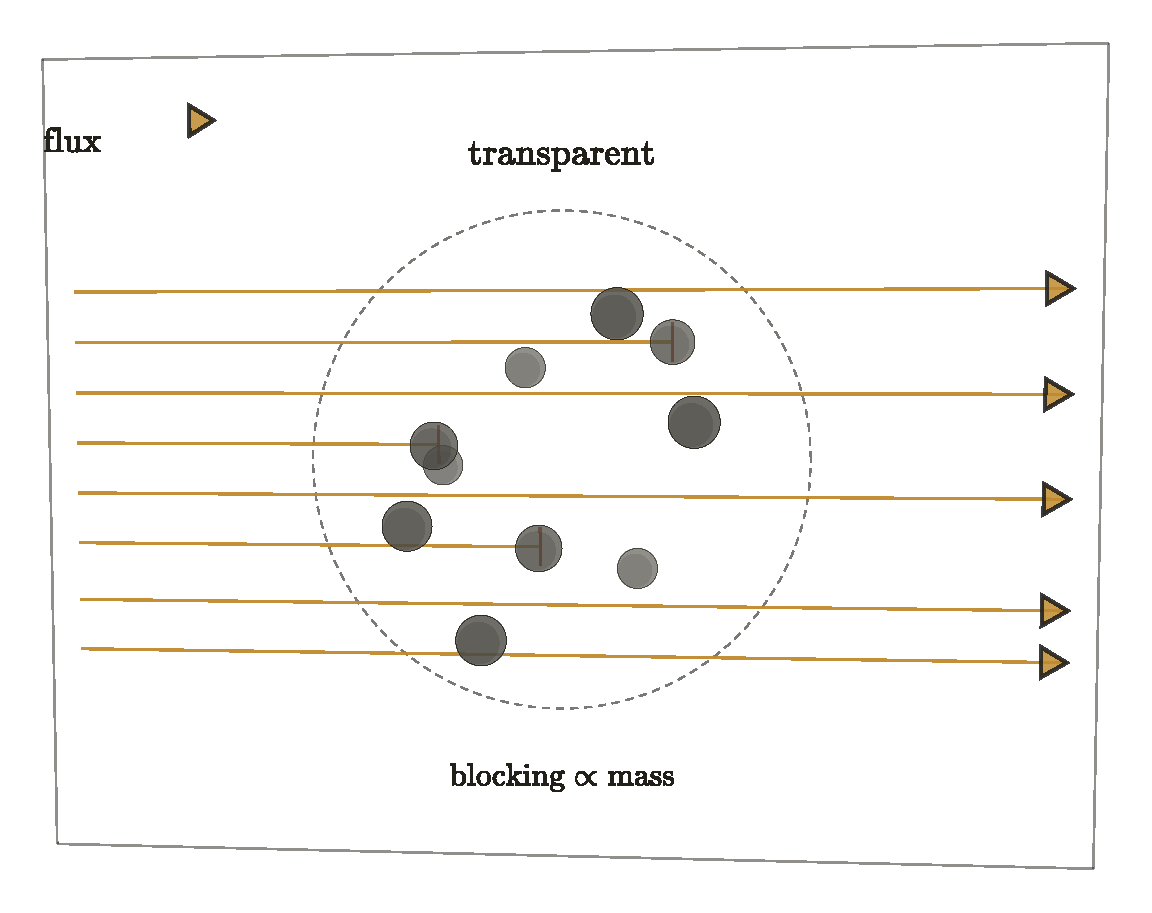
\includegraphics[width=0.60\textwidth]{figures/bbu_sixthwound_transparent}\\[0.6em]
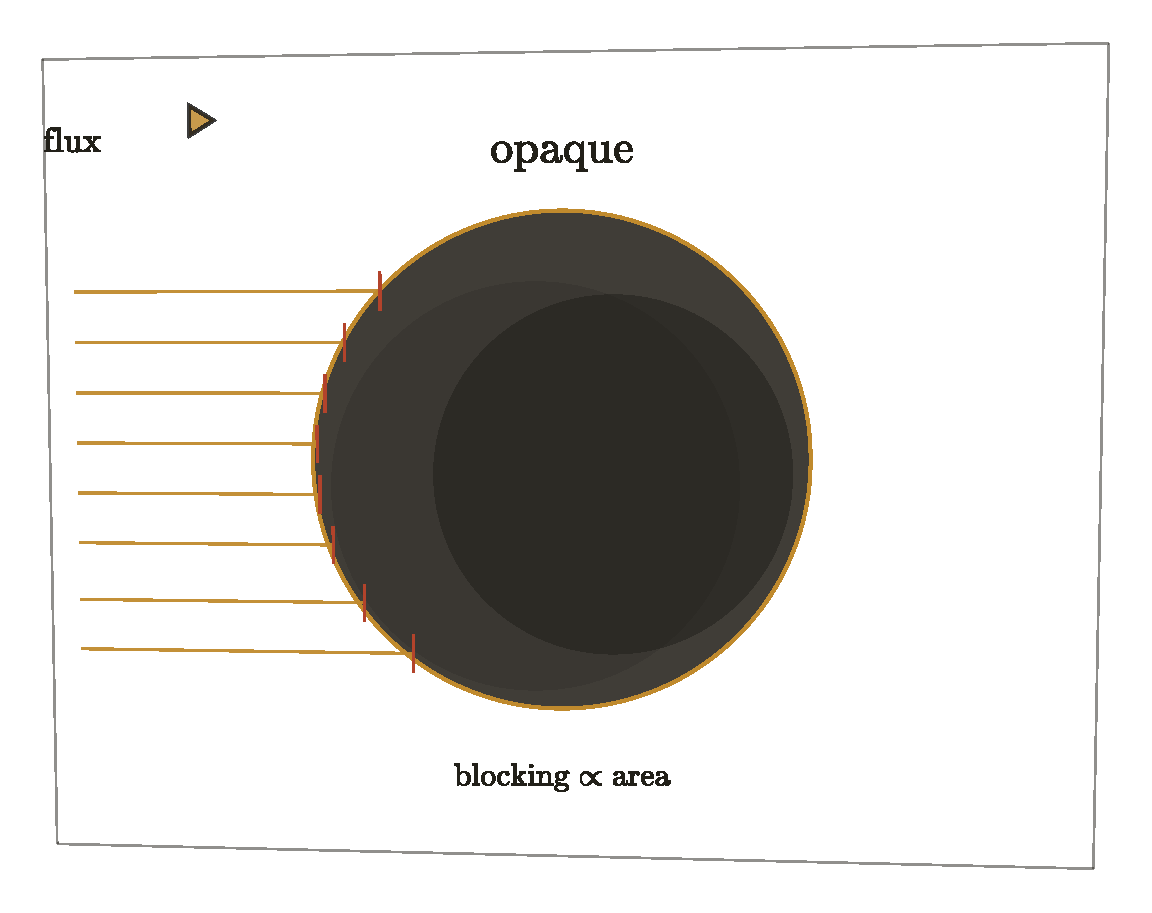
\includegraphics[width=0.60\textwidth]{figures/bbu_sixthwound_opaque}
\caption{The two regimes, which are the whole of this wound. Both panels show the same body under the same rain, drawn at the same size, differing only in how densely the matter inside is packed. Above: matter that stops only a little of what crosses it. Every piece blocks on its own account and nothing stands in anything else's shadow --- the rays that end do so one at a time through the depth --- one, in this drawing, past the centre --- because the interior is still being struck. The shadow counts all the matter, and the push follows the body's \emph{mass}. Below: the same outline packed dense enough to stop very nearly everything. Every ray ends at the front face, and whatever lies behind stands in shadow and adds nothing, however much of it there is. The shadow counts only the outline, and the push follows the \emph{silhouette}. Double the matter in the upper picture and the shadow doubles; treble it in the lower and the shadow scarcely stirs. Gravity, wherever it has been weighed, follows mass. The shadow push therefore requires the upper picture everywhere --- including inside bodies that have fallen past the last rung we know of. That is a requirement, and not a result.}
\label{fig:saturation}
\end{figure}

Two regimes, then, and everything turns on which one the world is in. Physicists say optically thin and optically thick; I will say transparent and opaque. \emph{The shadow push works only in the transparent regime.} That is the requirement. The rest of this section is about whether the world meets it.

Everywhere we can weigh, it does, and obligingly --- and here I must first correct my own bookkeeping, because an earlier draft argued in the wrong variable. A shadow does not care how densely matter is packed; it cares how much matter the rain must \emph{cross} --- the mass stacked along the path, per square metre of silhouette, density times depth. In that currency the Earth is already a serious obstacle: nearly thirteen thousand kilometres of rock, some seventy million tonnes over every square metre --- and its gravity still counts every atom in it, which is as direct a measurement as anyone could want of how little of the rain is stopped on the way through. Nor does the testing stop there. Binary pulsars, neutron stars orbiting one another and keeping time better than most clocks, have their masses and their orbits checked against each other to many decimal places, and the checks pass~\cite{kramer2021} --- and a \Ix{neutron star} stacks roughly a hundred thousand million times more matter along the rain's path than the Earth does: ten million million million tonnes over every square metre. Eleven orders of magnitude deeper into the requirement, and it has held.

The question is whether it holds all the way. What of a body that has fallen past the last rung we know of, something dense enough to trap light?

Suppose such a body is opaque. Then the numbers come out wrong, and it is worth being careful about \emph{how} wrong, because the first version of this section was wrong in the toy's disfavour and I would rather be accurate than frightening. There is a famous relation in which a black hole's radius grows in direct proportion to its mass, and I reached for it. But that relation describes a \emph{horizon},\footnote{Horizon, from here to the end of the book: the \emph{event} horizon --- the surface around a collapsed body from inside which light cannot leave. Not Chapter~4's horizon, which was cosmological: the limit of what has had time to reach us. Same word, two different fences, and the book now switches fences.} and a horizon does no blocking; blocking is done by matter. A horizon is in fact a poor stand-in for matter, as its own numbers confess: the average density inside one falls as the inverse square of the mass, so that a hole of ten suns encloses matter at roughly nuclear density, the hole at this galaxy's centre encloses an average of about a tonne per litre --- a thousand times water --- and a hole of ten thousand million suns encloses an average thinner than the air in this room. Nothing thinner than air holds anything up. Whatever sits inside a large hole must sit far inside it, on a strut of its own, at a density set by that strut and not by the horizon.

Take the body seriously and the arithmetic is the ordinary arithmetic of solid things. We live in three dimensions, mass fills volume, and a body held at some characteristic stiffness has a radius growing as the cube root of its mass and therefore a silhouette growing as about the two-thirds power. Possibly weaker: real degenerate bodies are perverse about this, and white dwarfs actually \emph{shrink} as they gain mass. So an opaque collapsed body would push as roughly the two-thirds power of its mass, where the world insists the push grows as the mass itself. The two rules diverge as the cube root of the mass ratio --- a factor of about seventy-five between a hole of ten suns and the one at the centre of this galaxy, and about a thousand across the whole observed range of holes. And the right variable makes the contrast crueller still: measured by the mass stacked across their own diameter, horizons \emph{thin out} as they grow --- double the mass and the column across the disc halves --- so the biggest holes in the sky are, in the rain's terms, the most weakly shielded objects in it, even as their gravity grows in lockstep with their mass.

A push growing as the two-thirds power, against a world where it grows as the first: that is a discrepancy the sky would have caught. The mass of the dark object at our galaxy's centre can be read from the orbits of the stars swinging around it, and independently from the size of the ring the Event Horizon Telescope photographed~\cite{eht2022}; the waveforms of inspiralling pairs match general relativity using one mass throughout. A push that tracked outline rather than mass would show up as those numbers refusing to agree with one another. They agree --- though I must add, and the seventh wound collects the point properly, that every mass in that comparison is itself weighed gravitationally, so the agreement is softer than it looks.

So here is the wound, as plainly as I can put it --- and it is a different kind of thing from the five before it. The shadow push requires matter to be at least nearly transparent to gravity's massions. That requirement is verified up to nuclear density and not one step beyond; past that, at the one place we can still watch, the observations say it holds anyway. The toy does not predict that and cannot explain it. What the toy does is \emph{require} it --- and requiring something you cannot check is a real exposure, even when nothing has contradicted you.

I want to grade that honestly rather than dramatically, because the temptation to flagellate is strong and unhelpful. Nothing here refutes the sketch. No measurement disagrees with it; no theorem forbids it; the toy is, in a certain sense, indifferent --- it does not care what the stopping chance turns out to be, only that some value works. What has happened is that the value is being pushed toward an extreme, and an extreme value is a reason for concern rather than a verdict. If the chance must be small enough to leave even collapsed matter transparent, then it is a very small number indeed, and I would rather say so out loud than let it sit unremarked in the machinery.

And there is a reading of the same fact under which it is not a wound at all. That number is not bookkeeping. If massions are real, it is a physical property of a real thing --- how readily one of them is stopped --- and somebody who could reach the densities at which the shadow saturates would not merely be constraining this book. They would be measuring its particle. Of everything in this chapter, this is the one place where the toy might one day be shown to be \emph{true}, rather than merely left standing. Whether to file that under wounds or under hopes I am genuinely unsure. I have filed it here, because here is where the pressure is; but the reader should know that it cuts both ways.

The best reply I have is real, and it is not free. A horizon is our layer's \emph{optical} fact: it is defined by what our light cannot climb out of. The massions are not our light. They belong to a layer below ours, they move very much faster, and they are under no obligation whatever to be stopped by whatever stops a photon. A collapsed body may therefore be black and still nearly transparent --- opaque to us, and hardly there at all as far as the rain is concerned. Then the push tracks the mass, the orbits come out right, and the wound closes.

It closes, though, by assuming exactly what is in question. Nothing here \emph{derives} the transparency; it is asserted, and asserted about the one regime in which nothing can be measured. That is the wound, and it does not go away.

But I want to be careful not to make it bigger than it is, because there is a cheap complaint waiting here and it is the wrong one. The complaint runs: the toy now needs a very small number --- the massion's chance of being stopped, per unit of matter it crosses --- and small numbers chosen to fit are how mechanical theories have historically died. I do not think that holds. A small stopping chance is not a fudge; it is a physical property, of the same family as the one that lets a neutrino cross a great thickness of lead without noticing it is there, and nobody calls the neutrino tuned --- though the neutrino's smallness is \emph{derived}, from the masses of the particles that carry its force, while the massion's is free; the honest claim is only that smallness by itself is no crime. What a number like that does is not embarrass the theory but \emph{point}. It says something quite specific about the floor or two below us: that whatever massions are, they engage matter only rarely, and that whatever matter is at that depth, it is mostly not in their way. That is not a stopper. It is a description of the basement, obtained from the sitting room, which is the sort of thing this book has been trying to get all along.

There is a better reason to take the number seriously, and it is that the toy cannot choose it freely. It is pinned by three demands at once --- twice from below, once from above. It must be small enough, and the massions fast enough, that the first wound's drag and heating do not kill the planets. It must be large enough that the shadow it casts is the gravity we actually weigh. And it must now be small enough that matter crushed past the neutron rung stays nearly transparent. One number, three demands: the heat books and the transparency of collapsed matter press the stopping chance down, gravity's own supply presses it up, and that is enough to pin it. If some single value meets all three, that is not a fudge but a test passed, and passed against the odds. If no value does, the toy is finished, and finished cleanly. Either way the number is doing the honest work of a parameter that cannot be tuned in private.

What would settle it is that number, measured or derived, and with it the density at which the shadow saturates. If saturation lies far beyond even collapsed matter, the toy keeps its proportionality to mass, and the smallness of the number stops being an awkwardness and becomes a finding --- a constraint on what lies a floor or two beneath us, which is exactly the sort of thing a bottomless world ought to let us learn. If saturation lies nearer than that, the gravity of collapsed bodies must somehow be made to track their mass rather than their outline, and I do not see how. That is the sixth problem of the research programme below, and of the seven it is the one I would most like to see somebody take away from me.


Scoreboard: \emph{open --- the stopping chance pinned twice from below (the heat it must not deposit, the collapsed matter it must still cross) and once from above (the push it must deliver), and derived from none.}

\section{Seventh Wound: The Equal Fall}

This wound was not handed down by the tradition either. It was handed to me late, by readers hired to hurt the book --- the Note at the back says how --- and the book's own rules oblige me to record that, because it means the previous section's claim to have collected the strongest objections was, for a while, false. It is the oldest fact in gravity arriving as the newest bill. Drop a feather and a cannonball in vacuum and they fall together; Galileo said it, the Moon landing filmed it, and a satellite named MICROSCOPE has now flown titanium and platinum side by side around the Earth and bounded any difference in their fall at about one part in a thousand million million~\cite{touboul2022}. Everything falls alike, whatever it is made of, to fifteen decimals.

Now watch that fact bite this toy in particular. Gravity, here, is blocking: the push on a body is set by how much of the rain it stops. Stops --- \emph{with what}? If a massion is stopped by particles --- by count of protons and neutrons --- the toy dies on the spot, and it is worth seeing how fast. About one part in a hundred of every nucleus's mass is binding energy: not particles but arrangement, pure energy of assembly, and the fraction differs from element to element at the level of a part in a thousand. Titanium and platinum of equal mass then cast unequal shadows and fall unequally at a part in a thousand --- and the satellite says any inequality sits twelve orders of magnitude below that. So the specification, the third of this chapter's demands to arrive with a number attached: \emph{the shadow must be cast by energy itself --- joule for joule, at exactly the rate energy carries mass --- to fifteen decimals.} Binding energy must block rain precisely as well as the particles it binds.

I will say the hopeful thing first, because for once the toy has one, and it is the only picture of the three that does. Newton has the equal fall as a coincidence: two conceptually distinct masses, gravitational and inertial, that merely happen to agree. Einstein has it as an axiom: the \Ix{equivalence principle} is assumed at the front door. The toy could, in principle, \emph{derive} it --- because in a crowd, the coupling that casts the shadow and the coupling that resists the push may be one coupling. Inertia, in the sketch of Chapter~6, is itself a crowd effect; if weight and inertia are bought from the same crowd at the same counter --- perhaps a layer down, where the momentum is actually traded --- then their ratio cancels by construction and the equal fall is not a miracle but a receipt. Nothing derives this. It is a hope with a computation named, and I price it as a hope. But it is the right \emph{shape} of answer, and neither rival has even the shape.

The measurements that pin it are worth naming precisely, because two of the tests this chapter leaned on earlier turn out to lean back. The masses in the pulsar and silhouette comparisons are themselves weighed gravitationally, so a push that mistracked mass would move all those readings together --- the comparison is softer than I first sold it. The versions that escape the circle are these: the waveforms of inspiralling pairs, where one and the same mass must serve as both the source of gravity and the resistance to it; and a neutron star falling, together with its white-dwarf companion, in the gravity of a third --- a stellar triple in which the strong-field body and the ordinary one have been watched to fall alike to a few parts in a million~\cite{archibald2018}. The equal fall holds even for a body whose mass is a tenth binding energy. The specification above is not a formality; nature enforces it in the hardest case available.

That is the first room of this wound. The second is a bill this ledger has been dodging, and a referee would have named the dodge in a paragraph: \emph{the toy is a Newtonian force law, and gravity has been measured past Newton.} Four times, classically~\cite{will2014}. Mercury's orbit turns forty-three seconds of arc per century more than Newton allows. Light passing the Sun bends by twice the Newtonian value. Radio signals grazing the Sun arrive late --- the Shapiro delay. And orbiting pairs spiral inward exactly as gravitational radiation demands. Every one is a measured difference between Newton and the world; this book banks the pulsars and the inspirals as assets in the sixth wound while never charging the toy for the difference --- which is bookkeeping of a kind the rest of the chapter was written to forbid. So, charged now, in full.

The replies the toy can offer have shapes and no numbers, and each is admitted exactly once, on the discipline that ``a deeper layer does it'' is a solvent unless a computation is named. The bent light and the delay have the most promising shape: light here is the crowd's own song, and a crowd made denser near mass slows its song --- a medium with the right profile reproduces both effects at first order, and the doubling that famously killed the naive corpuscle is, in a medium, a statement about that profile, which nobody has derived from the shadow. The perihelion needs velocity-dependent terms in the force --- and velocity-dependence is precisely the regime where the first wound's market already trades. The inspiral needs radiation reaction in the quadrupole branch the wave wound already carries. Three reply-shapes, one admission rule --- a deeper layer invoked once per bill, with a computation named --- and zero calculations done. Scoreboard: \emph{open --- four measured differences, zero calculated replies: the largest unpaid bill in the book.}

\section{The State of the Wounds}

Seven wounds, seven responses, seven invoices. Here is the whole campaign in one place --- what each objection was, the best answer the toy can give, what the answer costs, and what remains genuinely open.

\begin{table}[htbp]
\centering
\footnotesize
\captionsetup{font=footnotesize, skip=6pt}
\setlength{\tabcolsep}{3.5pt}
\begin{tabular}{P{1.85cm}P{3.05cm}P{2.9cm}P{2.6cm}}
\toprule
\textbf{wound} & \textbf{best reply} & \textbf{price} & \textbf{still open} \\
\midrule
drag \& heat & momentum taken from the slow flux, energy handed down the faster layers; the gap refuses, the cascade removes & energy books close only regressively --- no first account; steadiness and shot-noise unchecked & Poincar\'e's arithmetic, run against the cascade \\
\addlinespace[1pt]
the wave in nothing & the crowd waves; transverse stiffness from the tension of its own circulations (the rotating-superfluid precedent) & a hidden rest frame (the Lorentz conspiracy); generic anisotropy & the wave sector entire: light's dipole pair, gravity's quadrupole pair, one $c$, nothing else \\
\addlinespace[1pt]
charge orientation & fast tumbling averages the plane away; only the sense survives & a second perfectly hidden passenger & Coulomb's scalar, derived not hoped; attraction matching repulsion, though made two ways \\
\addlinespace[1pt]
exactness & selection demands uniformity; resonance supplies exactness; genealogy propagates it & gaps must \emph{emerge} from the crowd, not be assumed & the twelve decimals; the small, strange catalogue \\
\addlinespace[1pt]
the correlations (Bell) & sub-layer channels --- the lower layer's own light --- in the frame already bought and hidden: Bell's recommended ether & a second conspiracy: fast channels that can never signal & the Bancal fork: channels unbounded, or a signal one day outruns light \\
\addlinespace[1pt]
the saturated shadow & a horizon is our layer's optical fact, not the massions': a collapsed body may trap light and still pass the rain & transparency \emph{assumed} where it cannot be measured; the stopping chance pinned twice from below, once above --- derived from none & verified across eleven orders of crossed mass; where, if ever, does the shadow saturate? \\
\addlinespace[1pt]
the equal fall & weight and inertia bought at one counter --- the ratio cancels by construction (underived) & the shadow must price energy itself, joule for joule, to fifteen decimals & perihelion, bending, delay, decay: booked, unpaid \\
\bottomrule
\end{tabular}
\caption{The state of the wounds.}
\label{tab:wounds}
\end{table}

Two purchases recur in the table's price column --- the hidden rest frame bought for Michelson--Morley, and the downward regress of energy with no last account --- and one assumption, \emph{lower layers are faster}, does duty in two separate rescues. A toy whose escapes keep spending the same two coins --- that frame, that regress --- is either running out of money or telling you what its money is. And one more caution, applying the chapter's own rule to its own bookkeeping: economy is not evidence. A single unobservable device --- the layer below --- deployed four times is one assumption, not four survivals; the recurrence earns the toy nothing --- what it earns is only a sharper statement of what must be true if the toy is.

The state of the wounds can be read twice. Read forward, it is a defence: seven attacks, seven replies, seven invoices. Read backward, the same rows are a description of the layer below, assembled from measurements made at this one --- the reading the second, sixth, and seventh wounds each found for themselves, and which I did not see whole until the chapter was finished. Every survival above was bought by conceding what the basement must be like, and the concessions, collected, are no longer nothing: a crowd transversely stiff yet swimmable, carrying exactly two branches --- light's dipole pair, gravity's quadrupole pair --- at one speed, with no sound-like mode at all, its rest frame never showing; matter gapped and exact, sealing each layer's books; the whole of it nearly transparent to the flux, across eleven orders of crossed mass and the visible reach of gravity; and channels one floor down that outrun our light, in the frame already hidden. All of it conditional --- the specification of a thing not shown to exist --- and almost all of it qualitative. It is the first wound --- drag and heat, which until this page has only taken --- that supplies two of the three quantitative rows: the flux's speed floor and the heat refusal both trace to Poincar\'e's arithmetic. The equal fall arrived carrying its own number, the only wound to do so. To spare the orbits, the flux must move at no less than $24\times10^{17}$ times the speed of light --- so the assumption the wounds table prices as doing duty in two rescues, \emph{lower layers are faster}, has its first rung measured, and by the toy's executioner. And the heat figure --- one part in $10^{33}$ --- is the price on the cascade's work. The demanded intake is some $10^{20}$ times the sun's whole output, while the Earth's entire outflow of internal warmth --- about fifty million million watts, and geology has already spoken for it~\cite{daviesdavies2010} --- is a vanishing fraction of that. Whatever the first wound's escape does with the energy, then, it leaks into our thermometers less than roughly one part in $10^{33}$ of it --- a bound that only tightens, since the speed is a floor and the heat rides with the speed. The gap of the exactness wound stops being a hope with a job and becomes a component with a specification: the refusal just computed, thirty-three orders deep.

I take back at once half of what that seems to give. A specification is what a hypothesis must satisfy, not evidence that it does; the toy earns nothing --- not a hair of probability --- from the precision of the figures that nearly killed it, and this reading sits downstream of the refutations, never in their place. \Iy{Poincar\'e}'s numbers are still not figures a model recovers from; they are figures a survivor would have had to live by. And the crossroads here already has a name in this chapter: \emph{specification or epitaph}. The last specification of this extremity that physics wrote was the ether's --- the solid you could walk through --- and it was an epitaph. The wave wound stood at that same crossroads and recorded which way I moved; its comfort was a laboratory address. These two demands have no laboratory address --- nothing in any glassware moves at a million million million times the speed of light --- and what they have instead is a coincidence the correlations already recorded: \emph{lower layers are faster} was demanded twice, for unrelated reasons --- once to spare the orbits from drag, once to carry the correlations --- and here it is needed a third time. Agreement is thinner than glassware. I price it accordingly, and I keep it, for what it hands the programme below: the first problem's arithmetic now has its starting numbers --- supplied by the prosecution.

Seven problems, then, constitute the toy's open research programme, and I state them as problems, not as hopes. First: run Poincar\'e's arithmetic against the cascade --- quantitatively, with the layer speeds as parameters --- and see whether the drag, the heating, and the observed steadiness of gravity can coexist in any corner of the parameter space. Second: exhibit a circulation-strung crowd whose wave sector contains exactly two transverse branches --- a dipole pair for light and a quadrupole pair for gravity --- isotropically, at one fixed speed, and nothing else; or prove no such crowd exists. Third: build the tumbling-charge model and derive from it Coulomb's orientation-blind inverse square, or watch it fail. Fourth: show that gapped, exact, reproducible excitations --- the electron to twelve decimals, and a catalogue that is small and strange in the observed way --- can emerge from continuous crowd mechanics; the analog-gravity literature is the standing invitation. Fifth: settle Bancal's fork --- either derive no-signalling in the tower's unbounded limit, as quantum mechanics long ago did for its own; or, if the channels are finite after all, derive the equilibrium that hides them and say where it fails. Sixth: fix the massion's stopping chance per unit of matter --- transparency being already verified, by pulsar timing, across eleven orders of magnitude in the mass the rain must cross --- and settle whether one value of it can meet at once all three demands laid upon it: small enough, with the massions fast enough, for the first wound's drag and heating; large enough to supply the gravity we weigh; and small enough to leave collapsed matter transparent. If one value does all three, that is a test passed against the odds. If none does, the toy is finished, and finished cleanly. Seventh: derive the equal fall --- show that the coupling which casts the shadow and the coupling which resists the push are one purchase, so that weight and inertia cancel to the measured fifteen decimals; and compute even one of the four classical differences --- the perihelion, the doubled bending, the delay, the decay --- from the toy's own medium. Any one of the seven, solved in the toy's favour, would be a result. Any one solved against it would be a tombstone honestly earned. That is what a toy with content looks like: it can lose.

\section{A Wound That Runs the Other Way: Entropy}

Before the lessons, one entry runs the other way --- a place where the demand lands on the standard, bottomed picture, and the endless tower, for once, is the one making it.

\Ix{Entropy} has a dirty secret, and every physicist knows it and few say it plainly: it depends on \Ix{coarse-graining}. Entropy counts microstates per macrostate --- the number of fine arrangements that look the same from a distance --- which means it depends on where the line is drawn between what you track and what you ignore. Drawn by \emph{whom}? The flat picture is embarrassed by the question: entropy is supposed to be the most objective quantity in physics, and its definition smuggles in a choice. The embarrassment has a famous name --- the \Iy{Gibbs paradox}, in which the entropy of mixing two gases appears or vanishes according to whether the experimenter can \emph{tell the gases apart} --- and though quantum indistinguishability settles the practical cases, the conceptual question --- \emph{who} draws the line --- has stayed alive for a century and a half~\cite{jaynes1965}. The tower closes it, by supplying what the flat picture lacks: a physical ladder of coarse-grainings, not chosen but built. \emph{The entropy at layer $N$ counts the arrangements of layer $N{+}1$ that are indistinguishable from layer $N$.} The line is drawn by the world, once per layer. Entropy becomes layer-indexed --- fully real and fully relative at once, which the reader will recognize as this book's oldest principle wearing thermodynamic clothes: locally defined, globally unprivileged. And note what underwrites the count. It is the fourth wound's exactness: ``number of arrangements'' has a clean meaning only because the pieces come in identical species. Identicalness is not only stability's demand and the seal on the layer's books --- it is the precondition of thermodynamics itself.


\begin{figure}[htbp]
\centering
\begin{tikzpicture}[>=stealth]
  % top: layer-N view
  \node[anchor=south] at (4.8,5.08) {\small as seen from layer $N$};
  \draw[line width=0.9pt] (3.3,3.0) rectangle (6.3,5.0);
  \fill[black!30] (4.25,4.25) ellipse [x radius=0.55, y radius=0.40];
  \fill[black!30] (5.35,3.65) ellipse [x radius=0.55, y radius=0.40];
  % bottom: three N+1 arrangements
  \foreach \ox/\pat in {0.0/1, 3.5/2, 7.0/3} {
    \draw[black!60] (\ox,0) rectangle (\ox+2.6,1.8);
    \draw[dashed, black!35] (\ox+0.85,1.15) ellipse [x radius=0.50, y radius=0.36];
    \draw[dashed, black!35] (\ox+1.75,0.62) ellipse [x radius=0.50, y radius=0.36];
  }
  % distinct dot arrangements per box (same blobs, different micro)
  \foreach \p in {(0.62,1.22),(0.95,1.02),(1.12,1.3),(0.78,1.28),(1.05,1.14),(1.62,0.55),(1.9,0.72),(1.72,0.78),(2.02,0.55),(1.55,0.68)}
    \fill[black!60] \p circle (0.045);
  \foreach \p in {(4.12,1.1),(4.42,1.28),(4.58,1.05),(4.28,0.98),(4.6,1.25),(5.02,0.72),(5.32,0.58),(5.5,0.74),(5.18,0.5),(5.42,0.66)}
    \fill[black!60] \p circle (0.045);
  \foreach \p in {(7.68,1.3),(7.9,1.06),(8.12,1.24),(8.02,0.98),(7.62,1.08),(8.6,0.62),(8.82,0.76),(9.05,0.58),(8.72,0.5),(8.95,0.72)}
    \fill[black!60] \p circle (0.045);
  % arrows up
  \draw[->, bbuGold] (1.3,1.86) -- (4.35,2.94);
  \draw[->, bbuGold] (4.8,1.86) -- (4.8,2.94);
  \draw[->, bbuGold] (8.3,1.86) -- (5.25,2.94);
  % under-label
  \node[anchor=north, align=center, text width=8.8cm] at (4.8,-0.22)
    {\small three of the very many layer-$N{+}1$ arrangements that look identical from layer $N$ --- the count of them is the entropy};
\end{tikzpicture}
\caption{Entropy, layer-indexed. Above: a region as layer $N$ sees it --- two bodies, and that is all layer $N$ can say. Below: three of the very many layer-$N{+}1$ arrangements that present exactly this appearance. The number of such arrangements --- how many ways the crowd below can be while looking the same from above --- \emph{is} the region's entropy at layer $N$. The line between tracked and ignored is not chosen by an observer; it is drawn by the world, once per layer --- and the exactness of the crowd's species (the fourth wound) is what makes the count well defined.}
\label{fig:grainladder}
\end{figure}

Second, the arrow. Each layer's objects are made of \emph{many} objects of the layer below, so ``downward'' is always the direction of vastly more degrees of freedom --- and the cascade of the first wound runs down the tower for the same statistical reason that heat runs into the larger reservoir. \emph{The \Ix{arrow of time} points down the tower.} Time's direction stops being a mystery bolted onto the laws and becomes geometry: the tower has a many-states direction, and that is the direction things happen in. And here the bottomed and the bottomless pictures come apart where it matters. A bottomed universe has a finite basement; \Ix{equipartition} eventually fills it; the \Ix{heat death} --- Kelvin saw it in 1852~\cite{kelvin1852} and it has shadowed physics since --- is mandatory. A bottomless tower has an inexhaustible basement: there are always more, faster, finer modes to spread into, and equilibrium need never arrive --- \emph{need} not, rather than cannot, because escape forever requires the drain's rates to keep ahead forever, and that is a property of the cascade's arithmetic, not of depth alone. The heat death is not the tower's fate. Two prices, both already on this book's account: if the drain has run forever, why is our layer not empty? --- resupplied from above with no first account, the same unpaid regress as ever; and the deep puzzle of why entropy \emph{began} low~\cite{albert2000} is re-expressed --- the tower must have started wound up, charged --- not dissolved. I mark the difference and do not blur it.

And third --- the entry I find almost too good --- the tower without gaps predicts a catastrophe that physics has already met, named, and cured. A gapless tower drains \emph{instantly}: infinitely many ever-faster modes below would soak up all energy at once, and nothing at any layer would last a moment. Physics encountered exactly this monster at the bottom of a single layer. It is the \emph{\Ix{ultraviolet catastrophe}}: classical equipartition\footnote{Equipartition is classical physics' sharing rule: in equilibrium, every independent way of moving gets the same average energy. Harmless among few modes; catastrophic among infinitely many. (Dictionary.)} into the infinitely many short modes of the radiation field\footnote{The radiation field is light itself, considered as a thing that fills space; its modes are the distinct ways it can vibrate --- infinitely many, and ever shorter.} demanded infinite energy, every glowing coal an apocalypse --- and the cure, in 1900, was \Iy{Planck}'s quantum~\cite{planck1900}: a \emph{gap}, invented for precisely the job of throttling an infinite basement. (The man who later gave the catastrophe its name, in 1911, was Paul \Iy{Ehrenfest}~\cite{ehrenfest1911} --- the same Ehrenfest whose 1917 theorem on the three dimensions of space stands in this book's earliest notes. He guards both doors of this house.) So the gap, by the end of this chapter, has added a third duty to the two services already on its record: it keeps each layer's energy books exact, because below the first step nothing is absorbed or shed; it routes the gravitational intake past our thermometers, because what cannot be sipped is passed down whole; and it slows the leak downward that would otherwise empty our layer in an instant --- Planck's constant\footnote{Planck's constant, $h$, sets the size of the quantum --- the smallest step by which nature's gapped systems can absorb or emit. In this book's terms: the width of the throttle. (Dictionary.)} as the measured conductance of our layer's floor. A gapless tower dies of the ultraviolet catastrophe in an instant. A gapped tower has an arrow of time, and a future.

So the entry reads, on the other side's invoice: the bottomed picture owes a brute initial condition it cannot explain and a heat death it cannot avoid. The tower re-prices both --- the arrow as geometry, the death postponed by inexhaustibility --- at its standing price, plus the gap it was already carrying for three other reasons. This is not a proof that the tower is true. It is evidence of the only kind this chapter respects: a structure whose separate rescues keep turning out to be the same part, already installed.


\section{The Ladder Under Load: What a Star Does When It Loses}

There is a complaint I would make against this book if I were reading it rather than writing it. It has argued, for six chapters, that the world is layered without end --- and it has never once shown the tower under stress. Every picture so far has been of a universe going quietly about its business: rain falling, shadows overlapping, crowds holding their shape. A tower that only has to stand still is not much of a tower. What happens when you lean on it?

The universe runs that experiment for us, on a schedule, in public. The apparatus is called a star, and the experiment begins when the star runs out of fuel.

A star is a long argument between two pressures: the crowd pressing it inward, and the heat of its own burning pressing outward. When the fuel is gone the heat fails, and the star falls inward until something else stops it. Something else does. In a star of modest mass the something is the electrons: crowded past a certain closeness they refuse to be crowded further --- not because they repel one another, though they do, but because the world will not permit two of them into the same state. That refusal is stiff enough to hold the mass of the sun in a ball the size of the Earth.\footnote{Degeneracy pressure: the stiffness that arises because identical particles of certain kinds cannot occupy the same state. It is not a force between them; it is a prohibition on their arrangement. (Dictionary.)} The result is a \Ix{white dwarf}, and our own sun will make one.

Load it further and the electrons lose. Above about one and a half times the mass of the sun~\cite{chandrasekhar1931} --- \Iy{Chandrasekhar} computed the figure at nineteen, on the voyage from India to England~\cite{wali1991} --- the electron strut buckles, electrons are crushed into protons, and what stands up out of the wreckage is a body made almost entirely of neutrons: the mass of a sun inside the space of a city~\cite{baadezwicky1934cr}. The neutrons hold in their turn, by the same refusal plus the shove of the strong force, until something over two solar masses, where the neutron strut buckles too~\cite{oppenheimervolkoff1939,fonseca2021}.

And then, in the standard picture, there is more than an absence --- there is a prohibition, and it deserves its theorem-names. Buchdahl proved in 1959 that inside general relativity no static sphere of matter, whatever its stiffness, can hold itself at less than nine-eighths of its horizon radius --- under mild hypotheses: static, pressure the same in all directions, density not increasing outward~\cite{buchdahl1959}. And Penrose proved in 1965, with almost no hypotheses at all, that once collapse forms a trapped surface\footnote{A trapped surface: the point of no return made geometric --- a closed surface from which even the outward-aimed light is dragged inward. Penrose's theorem needs nothing else to have formed.} the equations do not merely lack a strut; they run out of road --- the infall cannot be completed within the theory~\cite{penrose1965}. So ``no third strut is known'' understates the standard position: inside the standard theory of gravity, no strut of any stiffness is \emph{permitted}. The equations run on to a place where the density is infinite and the volume is nothing --- a singularity\footnote{Singularity: a point in a theory's predictions where a quantity becomes infinite. Physicists generally read such a point as the theory failing rather than as a description of something real.} --- and the physicists who use the word will tell you, without being pressed, that it is not a description of anything. It is the mark left where the theory stopped working. And I must charge the toy for what the theorems mean: the tower's next rung is not a modest extension of the standard story. If a strut exists down there, then past that depth gravity itself is not general relativity --- the toy is not filling a gap in the standard theory; it is replacing the standard theory exactly where the standard theory forbids the filling. That is a large purchase, and the ledger now shows it.

Look at the shape of that story, because the shape is the whole point. Each rung is the same event at a finer scale: a structure's resistance is exceeded, its constituents are crushed into a smaller arrangement, and the smaller arrangement's own stiffness takes the weight. Heat fails; electrons hold. Electrons fail; neutrons hold. That is not an analogy for this book's thesis. It is this book's thesis, observed, twice, in objects we can point a telescope at.

And now notice what is doing the holding, because this is where I must be careful with my own enthusiasm. Degeneracy pressure is not a force in the ordinary sense. The standard account calls it exclusion: two identical particles of certain kinds are not permitted into the same state, and the not-permitting is stiff enough to carry a star. As physics that is not in dispute --- the white dwarfs are up there. But as an \emph{explanation} it is, in this book's terms, unfinished, because a prohibition is not a push. A rule that forbids, with nothing doing the forbidding, is the same species of object as a force that pulls across empty space with nothing in between; I have spent seven chapters declining that, and I cannot take the decline back here merely because the prohibition is holding up something I want.

So let me write the debt where debts belong, in the open. If this book is right, exclusion is not a decree handed down but a congestion: something about two identical arrangements of the crowd that cannot be pressed into one region without the crowd itself objecting, and objecting harder the closer they are pressed. The materials for such an account are already lying in Chapter~6 --- matter, here, is circulation, and circulations sharing a region are not a neutral matter. I did not have the account when I first wrote that sentence, and I want to say so in the same breath as the claim, because this ladder is the best evidence the book has, and evidence that rests on an unexplained prohibition is evidence with a hole in the middle of it. Since then I have been to look, and the section after this one reports what is there: further along than I expected, and not far enough.

What survives is weaker and still worth having. Whatever the stiffness turns out to be made of, it evidently comes layer by layer: each rung has its own version of it, and therefore its own limit mass. This ladder of collapse is the tower seen edge-on, under load.

\begin{figure}[htbp]
\centering
\begin{tikzpicture}[>=stealth]
  % the load
  \draw[->, bbuBlue, line width=1.6pt] (0.55,7.45) -- (0.55,0.30);
  \node[anchor=south, bbuBlue] at (0.55,7.55) {\small the load};
  % observed rungs
  \foreach \y/\body/\strut in {%
    6.5/a star/heat holds,
    4.6/a white dwarf/electron degeneracy holds,
    2.7/a neutron star/neutron degeneracy holds} {
    \draw[line width=0.9pt] (1.35,\y) rectangle (5.65,\y+0.8);
    \node at (3.5,\y+0.4) {\small \body};
    \node[anchor=west, bbuGold, align=left, text width=2.9cm] at (5.9,\y+0.4) {\small \strut};
  }
  % the unknown rung
  \draw[bbuGold, dashed, line width=0.9pt] (1.35,0.8) rectangle (5.65,1.6);
  \node[align=center, text width=3.9cm] at (3.5,1.2) {\small a body, held --- one floor down, or two};
  \node[anchor=west, bbuGold, align=left, text width=2.9cm] at (5.9,1.2) {\small a strut we cannot name};
  % failures
  \foreach \y/\why in {6.1/fuel gone, 4.2/above $\approx 1.4\,M_\odot$, 2.3/above $\approx 2\,M_\odot$} {
    \draw[->, bbuRed, line width=1.0pt] (3.5,\y+0.30) -- (3.5,\y-0.30);
    \node[anchor=west, bbuRed] at (3.72,\y) {\small \why};
  }
  \node at (3.5,0.42) {$\vdots$};
  \node[anchor=north, align=center, text width=6.8cm] at (3.5,0.15)
    {\small how much further, we cannot see from here};
\end{tikzpicture}
\caption{The ladder under load. Each rung is the same event at a finer scale: a structure's resistance is exceeded, its constituents are crushed into a smaller arrangement, and that arrangement's own stiffness takes the weight. The first three rungs are observed --- our sun will make the second, and we have photographed the third. The standard picture has no fourth rung and puts a singularity there instead: everything, in no volume at all, which is a floor by another name. The tower's fourth rung is an ordinary thing in extraordinary circumstances --- a body, held up by the layer below.}
\label{fig:collapseladder}
\end{figure}

Which makes the top of the ladder the interesting place. The standard \emph{equations}, past the neutron rung, offer a completed infinity: everything, in no volume at all. The standard physicists mostly do not believe them --- the working expectation is that quantum gravity intervenes with new structure at some depth, which the reader will notice is this book's own move in different clothes; the disagreement is not whether there is structure below the last known rung, but whether the rungs ever stop. And a singularity taken at face value is what I have spent this book declining --- not because infinities are distasteful, but because \emph{and here it stops, and do not ask what it is made of} is the move Chapter~1 called cheating when it was an edge, and Chapter~3 called arbitrary when it was a floor. A singularity is a floor. It is the most extreme floor anyone has ever proposed.

The tower does not need it. Past the neutron rung there is another rung: the layer below, taking the load on its own strut. The matter is not destroyed and does not become infinite. It is crushed into an arrangement our layer has no words for, and held up by a stiffness our layer cannot measure.

Here I want to be careful, because there is an overclaim available and I do not want it. That the tower is endless is a claim about the \emph{world}; how far a particular star falls is a claim about an \emph{event}. The two readings use the same word and are not the same claim, and this book asserts the first. The tower has no floor.

The second reading rests on the second rule of Chapter~6 --- that what happens in a layer is local to that layer and its neighbours --- which is itself a conjecture and was labelled one where it was stated. If that rule holds, a collapse is not a plunge down an open shaft. It is a sequence of separate events, each one a floor being overwhelmed and handing the load to the floor beneath, and there is no reason for such a sequence to run forever and every reason to expect it to stop at the first floor stiff enough to take the weight. A black hole would then be a body that has fallen a rung, or a few, and is sitting there, held --- exactly as a neutron star sits held one rung below a white dwarf. It has a state. It has structure. It is simply not our layer's structure.

I believe that firmly, and I want to be exact about the standing of it: I cannot prove it, and I am not claiming the alternative impossible. I made that mistake once already, in Chapter~3, where I went in to prove that no bottom was \emph{possible} and had the impossibility taken off me by an opponent who was right to take it. A conjecture held firmly and an impossibility established are different objects, and confusing them is the one error this book has already paid for once.

And from the outside the difference does not show. A body that has descended one floor and a body descending without end present the same face: dark, dense, and censored. The horizon does not report the number. So the modest claim is the one the evidence carries --- some rungs below ours, and we cannot say how many --- and anyone who tells you the number is telling you more than they have. That includes the singularity, which is the claim that the number is infinite.

Which suggests the name is wrong. \emph{Black hole} was coined inside a picture in which there is nothing at the centre but a point of infinite density --- a hole, in the plain sense that there is nothing there. In this book's picture there is a great deal there: a very dense body, made of the layer below, doing what dense bodies do. Not a hole. A star a floor or two down, wearing a horizon.

And the horizon itself gets demoted, by machinery this chapter has already bought and paid for. The second wound gave every layer its own light and its own speed limit; the fifth wound spent that coin, buying channels below ours that outrun our light. Apply it here and the famous sentence changes meaning. \emph{Nothing escapes} means nothing escapes \emph{at our layer's speed} --- and the layer below is not bound by our layer's speed. Its light is faster. A horizon is a local ordinance, exactly as $c$ is: black at our layer, and not necessarily black at the next.

That has a consequence I did not expect when I began this section. What falls in does not reach a bottom and does not vanish. It goes down a layer. Whatever the standard picture means when it worries that information is destroyed at a singularity, the tower's version is milder and stranger: nothing is destroyed. It is demoted --- kept, in a currency our instruments do not read.

One more debt at this rung, and it has a famous name. Hawking argued in 1974, and gave the full account the next year, that horizons are not eternal: they radiate, faintly, and evaporate over spans beside which the universe's age is an afternoon~\cite{hawking1975}. The standard picture's deepest open problem --- what becomes of the information that fell in --- is a problem about that evaporation's endgame. Two admissions, then. First: the tower's demoted-but-kept horizon is, in the standard literature's terms, a cousin of the \emph{remnant} scenario --- collapse halts on a deep strut, something persists --- and remnant scenarios carry known objections, chiefly unbounded information held in bounded energy, which this book has not answered. Second: the toy as it stands says nothing about whether its collapsed bodies radiate at all --- Hawking's flux comes from quantum fields on curved spacetime, machinery the toy has replaced without yet supplying its own account of what, if anything, leaks. Filed as open, not answered: the evaporation question survives the demotion untouched.

Now the bill, because a section that only collects is a section this book does not print.

The first of the bill's items is already in the ledger: it is the sixth wound, and this section is where I found it: if a body dense enough to trap light also stops the rain, its push follows its silhouette instead of its mass, and the sky says otherwise. I will not run the argument again here. I record only that it was this ladder that turned it up, and that of everything in the chapter it is the piece I hold most loosely.

The second item looked like a debt and turned out, on inspection, to be a question about bookkeeping rather than about the world. Black holes are credited with an entropy, and it is famously proportional to the \emph{area} of the horizon rather than to the volume within~\cite{bekenstein1973}. The entropy section of this chapter counted arrangements in volumes, layer by layer, so a change of shape at a horizon wants explaining.

But recall what that counting was: never a fact about the region itself, always a fact about what the layer above can tell apart. And now notice \emph{where} a horizon is. It is not where the body is --- the sixth wound had to establish that the body sits far inside it, on a strut of its own. A horizon is the surface at which our layer's light gives out: which is to say, the surface beyond which our layer can no longer tell one arrangement from another. So of course the count our layer can make is a count across that surface. An area law is what layer-indexed entropy would naturally give at a censored boundary. It is a measure of our blindness, drawn on the edge of the blindness, and it would be strange if it came out any other shape.

Which suggests the puzzle was never quite the puzzle it appeared to be --- and the reader has met its twin already, a few pages back. The Gibbs paradox looked for a century and a half like a fact about gases and turned out to be a fact about the describer: the entropy of mixing appears or vanishes according to whether the experimenter can tell the gases apart. The area law has the same shape. It looks like a fact about what is inside a black hole, and on this book's reading it is a fact about where our light stops --- which is not where anything material is. The tower does not have to explain why the interior's states should be counted on a surface. It says they are not being counted at all; what is being counted is the boundary of our ignorance, and that boundary happens to be a sphere.

And the tower need not choose between the two counts --- the area law's and the interior's own --- because it has room for both. The area law is our layer's entropy of that region: what we, from outside, can distinguish. Whatever is down there has its own count at its own layer, and there is no reason on earth for the two to agree --- they are entropies of different descriptions, which is precisely what the coarse-graining ladder said all entropies are. The tower predicts that they differ, and which way: the layer's own count, taken from inside, exceeds our area-count from outside --- ignorance can only lose states, never invent them. I should say plainly that not everyone reads black-hole entropy this way; there are serious programmes that read it as a census of real interior states, and if that reading is right the tower owes an account of the interior and not merely of the view. But on the reading this book has used throughout, the area law is not a debt at all. It is the definition, doing what it was built to do.

One consequence, and I record it because it retires an idea of my own. I had thought the area law might be explained mechanically: the massions themselves stopped at the body's surface, the shell being all the outside can ever touch. That idea can be set down now. The area law belongs to the horizon, and the horizon is not the surface of anything material; a shell would have been answering a question that was never asked of it. What remains of the thought is not an asset but a hazard --- it is exactly the opacity that the sixth wound says would break the gravity.

So the section closes as the good ones do, with a gain and a bill on the same page. The gain is real: the tower's least testable claim --- structure below structure, without a bottom in sight --- turns out to be something the sky demonstrates twice over in objects we have photographed, and the one place where the standard picture openly admits an absurdity is the very place the tower does not need one. The bill is real too: the same collapsed bodies that make the case are where the mechanism is likeliest to fail. That is the trade this chapter keeps making, and I would rather own both halves than either.


\section{Where the Stiffness Might Come From}

I left a debt standing a few pages ago and I would rather report on it than let it sit. The ladder's whole force depends on a strut I could not account for: degeneracy pressure, which the standard picture explains by a prohibition, and which this book may not explain that way, because a prohibition with nothing doing the forbidding is the same species of object as a pull across empty space. So I went looking at the one place in nature where circulations are packed together and \emph{measured}. What is there does not settle the question. It does narrow it, and it narrows it to a single line, which is worth more than a page of hedging.

Cool helium far enough and it becomes a superfluid, and it acquires a strange refusal: set the vessel spinning and the liquid declines to spin with it. What it does instead is thread itself with whirlpools --- vortices, each a line with the fluid turning around it --- and the whirlpools take up the rotation between them. The circulation of each one, meaning the flow summed around any loop enclosing it, is not roughly the same from vortex to vortex. It is \emph{exactly} the same: a fixed quantum, $\kappa = h/m$, about a ten-millionth of a square metre per second in helium, with $h$ Planck's constant and $m$ the mass of one atom~\cite{onsager1949,feynman1955}. You cannot have two thirds of a vortex, and the quantum has been measured directly~\cite{vinen1961}. Around each, the fluid turns at $\kappa/2\pi r$, and at the centre is a core about an \aa ngstr\"om across where the fluid simply gives out.\footnote{The core radius is set by the \emph{healing length}: the distance over which a superfluid can change its density. Inside it the superfluid has been destroyed; the vortex is a hole with a whirl around it.}

Now put that quantum to work, because it hands over the very thing the strut needs. Confine a circulation to a region of size $d$ and its speed there must be $\kappa/2\pi d$; so its momentum is
\[
p \;=\; m v \;=\; \frac{m\kappa}{2\pi d} \;=\; \frac{h}{2\pi d} \;=\; \frac{\hbar}{d},
\]
and notice what fell out of the arithmetic on the way: the mass cancelled. Squeeze a circulation into half the room and it must turn twice as fast, for the plainest reason there is --- the circulation it carries is fixed, and a fixed circulation in a smaller loop is a higher speed. That is precisely the confinement relation that degeneracy pressure runs on, and here it arrives with a mechanism under it instead of a decree.

Follow it one step further. Pack such circulations one to a cell of size $d$, so that the number in a unit of volume is $n = 1/d^{3}$. Each carries momentum $\hbar/d$, hence an energy of order $\hbar^{2}n^{2/3}/2m$; multiply by the number present and the energy in a unit of volume grows as $n^{5/3}$. That is the degenerate exponent \emph{exactly} --- the five-thirds that holds up white dwarfs --- and with the crudest geometry anyone could write down the size of it lands within a factor of about six of the real thing. (The derivation earns the strut. It does not earn the buckling --- why struts fail in a \emph{ladder} rather than all at once is bought separately, below, and only as a picture.)

I want to say what that does and does not prove, immediately, before the pleasure of it does any damage. It does not prove exclusion. The calculation assumed one circulation to a cell, and that assumption \emph{is} the exclusion; nothing came out that was not put in. What has changed is which half of the problem is missing. The kinematics --- why crowding forces motion, and forces it in exactly the proportion that gives the observed stiffness --- is now free, and comes from a fixed quantum of circulation rather than from a rule. The packing is not free. Why one to a cell?

The fluid has something to say about that too, and it is more than I expected. Start from two facts that are not in dispute: the energy of a circulation goes as the \emph{square} of its strength, and circulations add when seen from far enough away. Put two of the same sense side by side and, from a distance, they look like a single circulation of twice the strength: four units of energy, where the two of them apart cost only two. So a double quantum is not forbidden --- it is simply a bad bargain, and it splits. Which is exactly what doubly-quantized vortices are observed to do~\cite{shin2004} --- observed, I should add, in systems with somewhere to shed the difference; the splitting is energetics plus a channel to pay into, and the crowd must supply its own channel or the argument is only half made. That is not a prohibition against two things sharing a place. It is an arithmetic that drives them apart, which is what a mechanical account of exclusion would have to look like.

And the two senses are not symmetric. Opposite circulations \emph{cancel} at a distance rather than adding, so a pair of them costs almost nothing, attracts, and --- given, again, a channel to carry the energy off --- on meeting annihilates. Same repels; opposite pairs. The reader may notice the shape of something here --- the rule that lets two things into one place only if they are opposite --- and I want to be careful to say that this is a shape and not yet a derivation.

\begin{figure}[htbp]
\centering
\begin{tikzpicture}[>=stealth]
  % ---- (a) same sense ----
  \begin{scope}[xshift=-3.1cm]
    \draw[dashed, black!45] (0,0) ellipse (2.15 and 1.15);
    \foreach \cx in {-0.85,0.85} {
      \draw[bbuBlue, line width=1.0pt] (\cx,0) circle (0.55);
      \draw[->, bbuBlue, line width=1.1pt] (\cx,0) ++(72:0.55) arc (72:108:0.55);
      \draw[->, bbuBlue, line width=1.1pt] (\cx,0) ++(252:0.55) arc (252:288:0.55);
      \fill[black!70] (\cx,0) circle (0.05);
    }
    \node[anchor=north, align=center, text width=4.6cm] at (0,-1.35)
      {\small (a) same sense: from outside, one circulation of twice the strength\\ $\oint = 2\kappa$ \quad energy $\propto 4$};
  \end{scope}
  % ---- (b) opposite sense ----
  \begin{scope}[xshift=3.1cm]
    \draw[dashed, black!45] (0,0) ellipse (2.15 and 1.15);
    \draw[bbuBlue, line width=1.0pt] (-0.85,0) circle (0.55);
    \draw[->, bbuBlue, line width=1.1pt] (-0.85,0) ++(72:0.55) arc (72:108:0.55);
    \draw[->, bbuBlue, line width=1.1pt] (-0.85,0) ++(252:0.55) arc (252:288:0.55);
    \fill[black!70] (-0.85,0) circle (0.05);
    \draw[bbuRed, line width=1.0pt] (0.85,0) circle (0.55);
    \draw[->, bbuRed, line width=1.1pt] (0.85,0) ++(108:0.55) arc (108:72:0.55);
    \draw[->, bbuRed, line width=1.1pt] (0.85,0) ++(288:0.55) arc (288:252:0.55);
    \fill[black!70] (0.85,0) circle (0.05);
    \node[anchor=north, align=center, text width=4.6cm] at (0,-1.35)
      {\small (b) opposite senses: from outside, nothing at all\\ $\oint = 0$ \quad energy $\propto 0$};
  \end{scope}
\end{tikzpicture}
\caption{Why two like circulations are a bad bargain. Energy goes as the square of circulation, and circulations add at a distance. (a)~Two of the same sense look, from far enough away, like one of twice the strength: four units of energy where the two of them apart cost two --- so a double quantum splits, as doubly-quantized vortices are observed to do. (b)~Two of opposite sense cancel at a distance, cost almost nothing, attract, and on meeting annihilate. Same and opposite are not symmetric. That asymmetry is the shape of the rule which admits two things to one place only in opposite senses --- the shape of it, and not yet the substance.}
\label{fig:circulationpair}
\end{figure}

There is a third fact, and it is the one that speaks to Chapter~7 rather than to Chapter~6. Rotate the helium harder and the vortices do not smear out and do not pile up: they arrange themselves into a lattice with a definite spacing, set by how hard you are rotating~\cite{feynman1955}. Press harder still and the spacing shrinks, until the cores touch --- and then the arrangement gives way and something else happens. That is a strut being overwhelmed, in a bucket, on a bench. If exclusion is congestion rather than decree, then congestion can be \emph{beaten}, and a ladder of collapses is exactly what one should expect. The account I do not yet have would not only explain the strut; it would explain why there is a ladder at all.

And the same relation pays once more, in a place I had not thought to look for it. The third wound has this book's charges \emph{tumbling}: turning end over end, so that what a distant body meets is an average over orientations. Suppose that tumbling is not a device introduced to save Coulomb's law but the thing itself --- suppose it is what physics calls \Ix{spin}, taken literally.

Physics declines to take it literally, and has an arithmetic reason. An electron carries angular momentum of half of Planck's constant over $2\pi$; ask how fast a small ball would have to turn to carry that much, and the answers are ridiculous. At the old classical electron radius the surface must move at a hundred and seventy times the speed of light. At the size experiment now permits --- no bigger than the hundred-thousandth of a proton quoted in the fourth wound --- the figure is nearer fifty million times. So the textbooks conclude, reasonably, that spin is not rotation of anything: it is an intrinsic property, possessed and not explained. Another floor.

The reader can see where this book must go. \emph{Faster than light} is a violation only against our layer's light, and this chapter has twice been obliged to say that our $c$ is a local ordinance and the floor below runs faster --- once for the waves, and again for the correlations, where the fifth wound bought sub-layer channels outright. A circulation whose parts move at fifty million times our light speed is unremarkable if it is a circulation of the layer below. The objection that removes literal spin from the standard picture simply does not bind here. That is not a proof that spin is rotation. It is the removal of the reason for saying it cannot be.

And the magnitude comes free, which surprised me. Take the confinement relation above --- a circulation of size $d$ carries momentum $\hbar/d$ --- and ask what angular momentum that is, about the centre: $L = p\,d = \hbar$. One unit. The $d$ cancels, and so does the mass: it does not matter how small the thing is or how heavy. A quantized circulation cannot help carrying angular momentum of order $\hbar$, because that is what a quantum of circulation \emph{is}. Spin, in this picture, is not a further property the electron happens to have. It is the stiffness of the last few pages, read around instead of across.

Stand back from the last few pages and there is a pattern in them I did not put there on purpose. One fact was assumed --- that a circulation carries a fixed quantum, and cannot carry half of one. From that fact alone came the momentum of a confined circulation, $p = \hbar/d$; the angular momentum it carries about its own centre, $L = pd = \hbar$; and, if one asks how much energy a circulation of a given turning rate holds, the answer $E = \hbar\omega/2$ --- again exactly, again with the mass and the size cancelling out. Three of the relations that the quantum century had to \emph{discover}, falling out of one geometric fact about a fixed quantity in a loop.

That makes me want to revise something this book said earlier, and I would rather revise it in the open than quietly. Chapter~7's fourth wound explained discreteness by \emph{resonance}: the guitar string, only whole numbers of half-waves fitting, and \emph{fitting has no almost}. I still believe that argument, but I now think it was answering a different question from the one I asked it. Resonance explains why the survivors are \emph{identical} --- a shape either fits or it does not, so those that fit are all alike. It does not really explain why there are lumps in the first place. For that, the better answer looks like the one this section has stumbled into: not fitting, but \emph{packing}. A quantity that comes in whole units because a half-unit is not a shape the world has. A crowd whose members sit a certain distance apart, which therefore cannot carry a wave shorter than twice that distance --- not because the short waves fail to fit, but because there is nothing there to do the waving. Discreteness as geometry, and not as harmony.

If that is right, then the gap --- the book's hardest-working part, which keeps each layer's energy exact, hands the gravitational throughput downward, silences the crowd's short waves, and holds stars up --- is not a further law of nature laid on top of the crowd. It is the crowd's own spacing, seen from above. Planck's constant would then be a fact about how tightly the floor below us is packed, which is exactly the sort of thing a bottomless world ought to be able to say, and exactly the sort of thing a world with a floor must simply declare. (Dimensional honesty: a spacing is a length and Planck's constant is an action --- length times momentum --- so the identification is a programme, not an equation: the crowd must convert its one length into one action through its one speed and one stiffness, and any such lattice generically disperses short waves; the wave wound's measured dispersionlessness --- all colours arriving together across half the universe --- is therefore the bill this idea must someday pay.)

I will not pretend the swap is free. Tight packing in the ordinary sense means a crystal, and a crystal has axes: light would run at different speeds along different directions, and the descendants of the Michelson--Morley experiment have excluded that to about a part in a hundred thousand million million --- the same bound the second wound leaned on when it said that Michelson and Morley's sensitivity has been improved a billionfold since. What the picture needs is a packing that is dense and disordered --- glassy rather than crystalline, isotropic on the average, with a shortest length but no favoured direction. Real glasses are like that, so the demand is not absurd. But notice the price, because it is the same coin the fourth wound has already spent: in a disordered packing, geometry decides what is possible only \emph{on the average}, and I wanted it to decide exactly. Somewhere between the glass and the crystal there would have to be a medium disordered enough to have no axes and regular enough to have one spacing, and I do not know whether such a thing can be had.

So I leave the two accounts standing side by side, with the labour divided: packing for the lumps, resonance for the likeness. It is not the tidy single answer I would have preferred to print. It is, I think, the honest one --- and of everything in this chapter it is the piece most likely to be superseded by somebody who knows more than I do about how dense disordered matter arranges itself.


Two things it does not give, and I will not pretend otherwise. It gives one unit and not a half --- and a thing that merely rotates always carries whole units; the half is the tether's business rather than the turning's. And a rotating ball of charge has a magnetic moment in a fixed ratio to its spin, which for the electron is wrong by a factor of two. So there are now three twos owed: the two answers a measurement will admit, the two turns that bring a tethered object home, and the two by which the electron's magnetism exceeds its turning. In the standard picture these are not three independent facts: they share a root, and the root is the half-unit of spin itself. \Iy{Dirac}'s equation ties that half-unit to the magnetic factor of two; the spin--statistics theorem, which is a separate result and a harder one, ties it to exclusion. Two derivations, one property underneath. I take that as the useful hint in the whole business. If the three are one fact here too, then whoever supplies the packing rule will not be paying three debts. They will be paying one.


Three difficulties, stated plainly, because this is the least finished thing in the book. First, straight vortex lines are effectively two-dimensional objects when it comes to packing, and the five-thirds above wants \emph{compact} circulations --- closed loops, rings --- packed in three dimensions; the book's particles would have to be of that kind. Second, vortices can cross and swap ends. They are not perfectly impenetrable, and any account will have to say why matter's circulations are stricter than helium's. Third and hardest: a superfluid is a condensate, which is to say a crowd of things that \emph{like} to share a state, and getting the opposite behaviour out of structures living in it is not free. Nor have I derived the factor of two --- the rule permits two things in a state, of opposite sense, not one, and my figure shows a shape where a derivation should stand.

But the hardest of these --- and the half-unit of spin along with it, for they are the same difficulty wearing two hats --- has been done before, by people who were not trying to help this book. It is an established result that structures in a purely bosonic medium can be quantized as \emph{fermions}, carrying half-integer spin: Finkelstein and Rubinstein showed the possibility in 1968~\cite{finkelstein1968}, and \Iy{Skyrme}'s model of the nucleon~\cite{skyrme1962} is the working example everyone knows: a soliton in a field of bosons which, quantized properly --- \Iy{Witten} settled that point in 1983~\cite{witten1983}, two decades after Skyrme proposed the model --- comes out as a spin-one-half fermion. The mechanism has a homely demonstration: a thing tethered to its surroundings is not returned to itself by one full turn, because the tethers come back twisted, and needs a second turn to undo them. Something embedded in a medium is tethered by construction. So the last difficulty is not a wall. It is a place where somebody else has already been.

What I have, then, is not an account. It is a specification with two of its three parts already lying about in laboratory glassware: a mechanism that forces motion under confinement, in exactly the proportion the stiffness requires; and an arithmetic that makes like circulations separate and opposite ones pair. The missing part is the packing rule itself, with its factor of two --- and until somebody supplies it, the ladder of Chapter~7 stands on a strut whose nature is described rather than derived. I would rather print the specification than pretend to the account.


\section{The Dark Part of the Inventory}

A reader who follows astronomy at all has been waiting some pages to ask a question, and it deserves a straight answer rather than a silence. On the standard accounting, most of the matter in the universe is of a kind nobody has ever handled. It does not shine and does not block light; it announces itself only by its gravity --- in the speed of stars at the edges of galaxies~\cite{rubin1980}, in the motions of galaxies within a cluster~\cite{zwicky1933}, in the bending of light around masses far greater than anything visible there. What does a universe of shadows and pushes say about that?

Less than you might hope, and I would rather set out exactly how much less than leave the impression of an answer.

Begin with what is \emph{not} a difficulty. This book is an account of how gravity works, not a census of what there is. In the shadow picture a body pulls its neighbour because it removes some of the rain that would otherwise have arrived from its direction --- so anything that stops massions gravitates, whether or not it has any dealings with light. Matter that blocks the flux and ignores our layer's photons is not forbidden here, nor even surprising; it is simply matter we cannot see. The toy takes the inventory from the astronomers and leaves it alone. That is not an evasion. It is the proper division of labour between a mechanism and a census.

Now the temptation, which is real, and which a sympathetic reader will feel before I do. This book's gravity has something the standard one does not: a natural distance, the length a massion travels before something stops it. Could the anomalies be \emph{that} --- gravity failing gently at great range --- rather than unseen matter? It would be a fine thing for the toy if they were. I have come to think they are not, and there are at least three good arguments against reaching for it, which are worth naming properly rather than gesturing at.

The first is about direction. If massions are absorbed along the way, then gravity at long range is \emph{screened} --- weaker than the inverse square, not stronger. What the rotation of galaxies demands is the opposite: more pull at the edges than the visible matter can supply. Absorption pushes the discrepancy the wrong way. It does not close the gap; it widens it.

The second is about what the anomaly keeps time with, and it is the argument I find hardest to answer. If the effect came from a mean free path it would set in at a certain \emph{distance} --- much the same distance in every galaxy, since the massions do not know whose galaxy they are crossing. It does not. Galaxies of very different sizes begin to misbehave at very nearly the same \emph{acceleration}~\cite{mcgaugh2016}, which is a pattern that a length cannot make. Whatever is happening is keyed to how hard gravity is pulling, not to how far one has gone --- and the threshold itself is strange company for any local mechanism: it sits within a small factor of the speed of light times the universe's expansion rate, a cosmological number surfacing in galactic dynamics, which no mean-free-path story explains and this book does not pretend to.

The third is about separation. There are collisions of galaxy clusters in which the mass, as measured by the bending of light, has come apart from the visible matter and sits to either side of it~\cite{clowe2006}. Any adjustment of the law of gravity is tied to where the visible matter \emph{is}; it has great difficulty producing gravity in a place where the visible matter is not.

And a fourth argument outranks the other three in the standard accounting, because it is written in the sky's oldest light. The ripples in the microwave background --- the acoustic peaks --- record the early universe ringing like a struck bell, and the pattern of peak heights separates matter that couples to light from matter that does not, decisively: about five parts of the dark kind for every one of the ordinary~\cite{planck2020}. That is not a statement about galaxy edges, where a modified force might hide; it is a statement about the whole primordial plasma, at an epoch with no structure to confuse it. Any story this book tells about \Ix{dark matter} must reproduce those peak heights, and no such computation exists. The door stays open; this is the measure of how heavy it is.

So I do not think this book explains the dark matter away, and I would rather say that plainly than leave the possibility lying about as decoration.

But I want to be equally careful in the other direction, because \emph{this is not an alternative to dark matter} and \emph{this has nothing to do with dark matter} are different sentences, and I mean only the first. A tower of layers is a large and strange structure and I do not pretend to know everything that follows from it. Something a floor below us that engages the massions and not our light would be, in this book's own terms, precisely what the standard picture would record as mass that cannot be seen. Whether that thought leads anywhere I genuinely do not know --- I have not been able to make it do any work --- and I set it down as an unexplored hole in the wall rather than as an answer. Marked holes are more useful than papered ones.

One thing does come back from the exercise, and it belongs to the saturated shadow --- the sixth wound. Gravity is observed to work across a galaxy, across a cluster of galaxies, and across the distances over which light is bent by masses lying most of the way to the edge of what we can see. If massions were being used up on the journey, gravity would fail somewhere along that range, and it does not. So the massion's mean free path must be at least as long as the greatest distance over which we can watch gravity operate --- which is a fourth demand on the stopping chance, arriving from the largest scales there are. It pushes the stopping chance the same way as the transparency demand rather than against it, so it does not tighten the pincer; what it does is stretch the range over which transparency must hold by a factor it is difficult to write down. A mechanical theory of gravity should be made to meet that, and this one is now on notice that it must.

Of the other darkness --- the accelerating expansion, and whatever is driving it --- this book has nothing whatever to say. It is an account of a mechanism, not a history of the universe, and it does not reach that far. I would rather be silent there than inventive.


\section{What That Teaches}

Seven wounds, and the table above holds their state. Let me draw the lessons, because they were the purpose of the chapter, and they are not the lessons of defeat.

The first lesson is about why the mechanical programme died, and it matters for how one should hold this whole book. It did not die of fashion, or dogma, or failure of imagination. It died of \emph{arithmetic} --- of Poincaré's numbers and Michelson's null and the scalar stubbornness of charge. The physicists who abandoned billiard balls loved billiard balls; they were driven out by calculation, wound by specific wound. Anyone reviving the demand --- as this book does --- owes those calculations respect, not resentment. The demand for mechanism is honourable. The nineteenth century's particular mechanisms are dead, and they were killed fairly.

The second lesson cuts the other way. The \emph{demand} did not die with the mechanisms, and modern physics knows it. The embarrassments that started this book --- action at a distance, the bending of nothing --- were never resolved; they were \emph{renamed}, wrapped in mathematics of great power and even greater silence about what anything is. And at the frontier, the demand keeps resurfacing in respectable dress: whole research programmes now ask whether spacetime is emergent, whether the vacuum is a medium's ground state, whether gravity is a statistical push rather than a fundamental pull~\cite{verlinde2011}. The child who said ``that is cheating'' has, at the very least, not been answered. He has been outvoted.

And the third lesson is the one I most want the reader to take. Every wound in this chapter exists because the toy made a \emph{claim}. Drag exists because the toy said what gravity is made of. The ether problem exists because the toy said what space is. The orientation problem exists because the toy said what charge is. A picture that said nothing would have suffered nothing --- and taught nothing, and been nothing. The scoreboard of this chapter, wounds and all, is the toy's certificate of seriousness. I said at the start that I love it no less for what the tests have done to it. Reader, having watched the tests: I love it somewhat more.

What remains, after the testing, is what remained after Chapter 3's battle, and it is fitting that the book's two hard chapters end on the same note. The grand claim is not established: I cannot hand you a mechanical universe that reproduces what we measure. The pincer is the reason --- not because it has been shown fatal, but because the escape this chapter offered it has never been calculated, and an uncalculated escape is not a rescue. What survives is smaller and unbroken: a universe with no magic in it is still the only kind I am willing to want --- and the places where the toy is weakest are not embarrassments to hide but \emph{addresses}: the exact locations where anyone who shares the demand should dig. The last chapter of this book says what I think we are entitled to keep. It is short, because after everything, what we are entitled to keep is one thing.

\En

\begin{draftnote}
Craft notes (fact-check pass done; cleared items live in ref.bib notes and FACTCHECK\_REPORT.md): (1) [Poincaré figures inserted in the pincer per PROSE\_PATCHES\_stage1.md; the stale deferral parenthetical removed on the author's ruling.] [resolved 2026-07-29: invoked twice (second wound; stiffness section) and verified --- Michelson--Morley 1887 probed $\Delta c/c$ at the $10^{-8}$ level (the expected $v^2/c^2$ of orbital motion); Herrmann et al.\ 2009 (PRD 80, 105011 = herrmann2009) reached $\Delta c/c \sim 1\times10^{-17}$: a billionfold, as the prose says, and the two passages agree with each other.] Electron substructure: [resolved 2026-08-21, and the number was corrected downward: the LEP contact-interaction bounds in the PDG listings run from about 8.5 to 26 TeV, i.e.\ $\sim2\times10^{-20}$ m at the weakest. That is ten thousand times smaller than a proton, not the hundred thousand the prose had claimed --- a hundred thousand needs the single most favourable model in the range. The fourth wound now says ten thousand and cites pdg2024.] All other item-1 checks (Maxwell critique, GW170817 bound, g-2, Kelvin re-emission) confirmed. (13, Entropy section) [resolved: Gibbs paradox statement checked against Jaynes 1965 (Am.~J.~Phys.~33, 391, now in ref.bib as jaynes1965) --- the book's gas-mixing formulation is the standard one; ``entropy is an anthropomorphic concept'' is \S{}VI of that paper, phrase credited by Jaynes to Wigner, should the author ever want it in prose. Kelvin 1852, Planck 1900, Ehrenfest 1911 coinage, and Albert's Past Hypothesis all confirmed earlier.] (12, Fifth Wound) [resolved: all citations confirmed; Bell attribution split in prose per PROSE\_PATCHES\_stage1.md --- ``cheapest'' is Bell's, ``least crazy'' marked as the author's.] (2) The condensed-matter/analog-gravity paragraph should eventually name names in an endnote --- Volovik's helium work, analog horizons in BECs, Verlinde's entropic gravity --- kept out of the main text to preserve voice. (3) [resolved: built as tab:wounds.] (4) [resolved: the Coda delivers exactly one thing.]
\end{draftnote}

% ---- Coda-reprise plate (ruled in 2026-08-20) ----------------------------
% The cover's own recursion, reprised full-page on the verso so it faces the
% Coda's open door across the spread: the endless world beside the one way out.
% No new asset -- this is the same master the cover is built from, printed here
% in the interior's grayscale. The parity guard puts it on a verso; \addchap
% then opens the Coda on the facing recto.
\clearpage
\ifodd\value{page}\hbox{}\thispagestyle{empty}\newpage\fi
{\thispagestyle{empty}\null\vfill
 \centerline{\includegraphics[height=0.86\textheight,width=\textwidth,keepaspectratio]%
   {cover/cover_recursive_ball}}
 \vfill}
\clearpage
\addchap{\emph{Coda --- One Mystery}}
\markboth{Coda --- One Mystery}{Coda --- One Mystery}
\chapterart{coda_open_door}
\draftstatus{Draft 1}

\lettrine{A}{} book should end by saying what it believes it has earned --- no more, and out loud.

This one began with a child's two complaints: that pulling through nothing is cheating, and that every border anyone drew only multiplied the questions it claimed to settle. The book grew up around the complaints, and along the way it lost things, publicly and on purpose. It lost the theorem the child wanted --- the proof that no bottom is possible; an artificial mind and I searched for it together and found, instead, the exact place where the proof is blocked, and we left the block standing because it would not move. It lost the easy version of the grand mechanical claim --- the toy universe of shadows and circulations did not come through its own Chapter 7 unmarked, and I graded its wounds myself, and paid for every answer in the open. It even lost the comfort of totals: in an infinite world there is no cosmic ledger to improve, and the ethics of this book had to learn to live, as everything in this book lives, locally.

So what is left? One thing. I promised it would be one thing, and it is this:

\textbf{A universe in which everything has a reason, except the one question that no universe of any kind could ever answer.}

Why is there something rather than nothing --- that question stands, and will stand, over every picture anyone will ever draw: over the brute floor, over the endless layers, over whatever physics is discovered next century, equally and forever. It is not this book's failure. It is the admission fee of existing at all, and every worldview pays it at the same window.

But past that window, the pictures differ, and this is the whole of what I have argued: they differ in \emph{how much more magic they ask you to swallow}. A universe with a bottom asks you to pay twice --- once at the shared window, and once more at its floor, that final layer of which you may not ask ``why this? why these properties? why here does asking end?'' A universe of endless layers pays once. Every level has its reason in the level below; no object acts without touching; no space is nothing pretending to be something; no border is painted where a question used to be. All of the arbitrariness --- every last unit of it --- is swept into the single point where arbitrariness was always going to live, and the rest of the universe is left clean.

One mystery. Not zero --- the child had to give that up, and it was right that he gave it up in a fair fight rather than keeping it by never fighting. But not two, either, and never the smuggled kind: not a mystery dressed as an answer, not a force that is really a leap, not a floor that is really a decision to stop asking. One mystery, sitting where everyone's mystery sits, and no magic anywhere else.

I cannot prove this universe is the true one. Chapter 3 shows exactly why not, and Chapter 7 shows how far the sketch of its machinery still is from the world's measured exactness. What I can say is what kind of claim it is. It is the same claim the child made, grown careful: that an explanation which stops arbitrarily has not finished, and that a world worth believing in is one where the stopping happens only where it must --- once, at the bottom of every possible question, and nowhere nearer.

And if the copies are real --- if the pattern that insists on this is not a private stubbornness but a recurring feature of an endless world, asking its question at every scale, in every direction, without end --- then somewhere far from here, and somewhere deep inside the matter of this page, another version of this book is ending now, on the same sentence, and its author believes what I believe:

that the universe owes us no answers --- but it owes us reasons all the way down, and all the way down is exactly what it has.

\En

\begin{draftnote}
Craft notes: (1) The Coda must be read against Ch. 7's closing line (``what we are entitled to keep is one thing'') --- the handoff works; keep the two in sync through revisions. (2) The final sentence deliberately fuses the book's two theses --- reasons all the way down (Part II) and the endless world (Part III); resist the urge to explain it. (3) Total length $\sim$650 words; it should stay under a thousand no matter what revision adds. (4) Consider whether ``the admission fee of existing at all... every worldview pays it at the same window'' earns a callback in the book's marketing copy; it is the thesis in one image.
\end{draftnote}

\addchap{\emph{Epilogue: The Aha Moments}}
\draftstatus{Draft 1}

\lettrine{T}{he} ideas in this book did not arrive in order, and they did not arrive at once. They arrived the way such things do --- as a string of ``Aha!'' moments, years apart, each one small at the time. Here is the string, as honestly as I can date it.

\begin{itemize}
\item \emph{Age eight, or near it} --- One evening when I could not sleep, my father explained that seeing is light bouncing from things into the eye, and the explanation \emph{satisfied} in a way nothing had before: a chain with no gaps. The standard by which everything since has been judged.
\item \emph{Age ten, or near it} --- Curved spacetime, from a television programme --- or it may have been radio; the verdict has outlived the source --- and the immediate, wordless response: \emph{this is clearly cheating.} Space is nothing; nothing does not bend.
\item \emph{The same year, more or less} --- The copies. An infinite universe, I realized, must contain another me --- and the thought comforted me at once. I told my brother; he was not comforted; Chapter~5 is my long answer to him.
\item \emph{Around twenty-five, and again around forty} --- The ideas returned, were turned over, and were put back. Little or nothing was written down. Some convictions are patient.
\item \emph{Around fifty --- about 2019} --- The notes, at last: massions, the rain, the shadow --- gravity as a push and not a pull, written down in Danish and put in a drawer, taken out and touched up every so often in the years since. Charge as circulation --- orientation and sense of rotation standing in for plus and minus, annihilation as two gears finally allowed to unwind --- arrived in the same season.
\item \emph{2026} --- The seven rounds with Kai. I went in to prove that no bottom is possible; I came out with something smaller and stronger: not \emph{more grounded} --- \emph{less arbitrary}. One mystery instead of two. The proof I wanted is blocked, and the block is in the book, standing.
\item \emph{2026} --- The weeks of the wounds: the elastic escape and its burial; the two plates and the cancelling ten percent; the cascade that sells energy down the tower; entropy turning out to be the other side's invoice; and light, at the very end, revealed as the crowd's own song. The toy stopped merely surviving and began to pay out.
\end{itemize}

Much of this book is speculative --- inevitably so --- and the text has tried to say, every time, exactly how speculative. The ideas themselves are mine; the objections mostly are not, and the book is better for every one of them. I owe the lineage --- Lucretius to Le Sage --- the debt one owes ancestors who failed in ways that can be learned from. I owe Kai, the expressed voice of everything the library holds, the debt one owes an honest opponent. And I owe the reader who has come this far the only closing the book permits: globally, nothing is special. Locally, you are. Thank you for reading locally, here, with me.

\addchap{\emph{A Note on How This Book Was Made}}
\draftstatus{Draft 1}

\lettrine{T}{here} is one more thing I owe the reader, and it is a plain account of how the object in your hands came to exist. I would rather give it than have somebody find it out, and I have a better reason than that, which I will come to at the end.

The ideas in this book are mine and they are old. The shadow push, the layers without a floor, charge as circulation, the copies, the local surplus: those were in my notes before I had any help writing them down, and the earliest of them were in my head before I could have defended them to anybody. The chronology in the epilogue is honest; nothing in it was supplied to me.

The sentences are another matter. Most of the prose in this book was drafted by an artificial intelligence working from my instructions, in a voice built deliberately from my own earlier writing, over a long conversation that ran to hundreds of exchanges. I set the arguments and the order; it proposed the words; I read every one of them and kept, corrected, or threw them out. Where it wrote something I would not have said, it was cut. Where it wrote something better than I could have, and true, it stayed --- and there are such places, and I am not going to point at them and blush.

It did other work, too, and the reader may as well know its extent. It drew most of the diagrams in code, so that their geometry would be arithmetic rather than eyeballing. The plates showing three-dimensional shapes go further: each states in advance what its own construction must satisfy --- that the grazing line really does meet the ball's radius at a right angle, that the blocked patch really is a quarter of its neighbour, that the small region marked in one panel really is the region the next panel magnifies --- and the program that made the figures in this book refuses to draw at all if one of those statements has stopped being true. I am fond of that arrangement, and not only because it caught mistakes. A picture that can fail its own test is the nearest thing a diagram can be to an honest witness.

I should say what it cannot do, since I have just made rather a lot of it. The assertions test the geometry the caption \emph{claims}; they cannot test whether the picture drawn from that geometry depicts it correctly. The distinction is not academic. One of these plates carried an error in the way it drew a sphere's outline --- enough to put a circle outside a ball it lies on --- through every check the plate makes, a clean lint, and a run that would have refused to write the file if any claim had failed. It was found by somebody looking at it. That is the shape of the whole enterprise, and it is worth stating plainly rather than discovering later: machines verify what they were aimed at, and eyes find the rest. It ran the fact-checking: every number, date, page reference and attribution in this book was fetched against a named source, and the corrections came back in a report I read and ruled on. Several of them were corrections to my own errors. Several were corrections to \emph{its} errors, caught by procedures we had agreed on in advance for exactly that purpose. Two of the seven wounds in Chapter~7 reached their final form because a machine told me a number I had used was wrong, and it was.

One more fact belongs here, under this note's own rule that I would rather give a thing than have it found out. No one but its author read this book before publication. The adversarial readers who wounded it --- the ones who forced the seventh wound into existence --- were machines, briefed to hurt it, and their reports are in the record. So the first person to test this book against a human chest is you, and the letterbox is open: the record's address is printed on the copyright page, corrections become errata, errata become the next printing. The book said it can lose. You are how it finds out.

The pictures that are not diagrams are machine work too, and of a different kind. The engravings at the head of every chapter and the Coda, the two full-page plates, and the ball on the cover --- which returns, in grey, to face the Coda --- were generated from written specifications of mine by an image model; no hand drew them, and I would rather say so here than have it noticed elsewhere. The cover's recursion --- a ball built of balls built of balls --- was beyond any single request, so I generated four pieces separately and assembled them into one myself. And one distinction, since this note has made much of diagrams that refuse to draw when their claims break: these can refuse nothing --- they decorate, they do not argue, and you could cut every one of them without moving anything in the case this book makes.

What that intelligence did not do was have the ideas, decide the physics, or supply the memories. It could not tell me whether my father explained light to me when I was eight. It could not decide whether the tower has a floor. When I told it that a collapsing star's descent need not be endless, it had the argument the wrong way round and said so; when I told it that a black hole's silhouette grows as the two-thirds power of its mass and not the square, it checked, agreed, and the sixth wound shrank to its true size. The judgements in this book are mine, and so is the responsibility for them.

Chapter~3 is a special case and I want to be exact about it. That dialogue is not a literary device. It is an edited record of an argument I actually had, with a machine, over many rounds, in which I set out to prove that a bottomless universe was the only possible kind and failed. The concessions in it run both ways, and mine are on the page because they are the most useful thing in the chapter. I lost that argument twice, and the book is better for it than the book I meant to write.

There is a record. The manuscript, the reference file, the fact-checking reports, and the whole trail of corrections with my approvals on them live in a repository that I intend to open to the public when this book is published. Anyone who wants to see the seams can see them.

And here is the better reason I mentioned. This book argues, for a hundred and sixty pages, that a thing is understood only when you can follow the chain of reasons under it, and that a wall with no explanation behind it is cheating wherever you find it. A book making that argument while concealing its own construction would be breaking its own rule on its last page. So: no magic here either. The ideas are mine, the labour was shared, the errors were caught by procedure, and you can go and look.

\appendix

\chapter{\emph{A Small Dictionary of the Terms}}

Entries are short on purpose: enough to keep reading, not enough to replace a textbook. Physics and philosophy share the alphabet here, as they share the book.

\paragraph{Action at a distance.} Influence that crosses empty space with nothing travelling between --- Newton's gravity as written, and this book's original grievance. The opposite is contact, or mediated, action.

\paragraph{Bancal's theorem.} If quantum correlations were carried by hidden influences at any \emph{finite} speed --- however far beyond light --- experimenters could exploit them to send faster-than-light messages. Nature shows none; so hidden channels must be unbounded or absent. The theorem that forces the choice this book calls the Bancal fork: channels of unbounded speed, or a prohibition that one day cracks --- the one place where the tower's endlessness itself does physical work.

\paragraph{Bell inequality; hidden variables.}\index{hidden variable} A hidden-variable theory says particles carry definite properties with them, and measurements merely reveal them. Bell (1964) proved every \emph{local} theory of that kind obeys a numerical inequality; quantum experiments violate it. The violation is the Fifth Wound.

\paragraph{Bohmian (pilot-wave) mechanics.}\index{pilot wave} Quantum mechanics rebuilt with particles that always have positions, guided by a wave. It reproduces every quantum prediction, is fully deterministic --- and is openly nonlocal, requiring a preferred frame.

\paragraph{Bose--Einstein condensate.} A dilute gas of atoms cooled until they occupy one shared quantum state; a laboratory superfluid, transparent to cameras. The vortex-lattice experiments of Chapter~7 live here.

\paragraph{Cascade.}\index{cascade} The toy's disposal route for absorbed energy: handed downward one layer at a time, each faster layer accepting what the slower one cannot keep, none of them warming. Christened in Chapter~6; stress-tested as the First Wound's only escape.

\paragraph{Circulation; vortex.}\index{circulation}\index{vortex} Flow that goes around --- the whirl of a vortex. In this book, circulation is the proposed substance of charge and the tension that lets a fluid carry transverse waves.

\paragraph{Coarse-graining.}\index{coarse-graining} Deliberately ignoring fine detail: counting arrangements as ``the same'' when they differ only below some scale. Entropy is defined relative to a coarse-graining; the tower gives the graining a physical ladder.

\paragraph{Crossed mass.} The mass the rain must pass through: density times depth, summed along the path --- tonnes per square metre of silhouette, not per cubic metre of packing. The sixth wound's honest currency: transparency is a claim about crossed mass, and it is verified across eleven orders of it.

\paragraph{Dark matter.}\index{dark matter} The name for whatever makes galaxies gravitate as if they held about five times the matter we can see. The evidence: rotation speeds, colliding clusters, and the pattern of ripples in the sky's oldest light. What it is remains unknown; Chapter~7's inventory prices the candidates, this book's own speculation included.

\paragraph{Degeneracy pressure.} The stiffness that arises because identical particles of certain kinds cannot occupy the same state: not a force between them but a prohibition on their arrangement. It holds up white dwarfs (electrons) and, with the shove of the strong force, neutron stars (neutrons), and in this book it is the gap doing structural work.

\paragraph{Diagonal theorems.}\index{diagonal theorems} The book's collective name for the G\"odel--Tarski--Russell family: any system rich enough to contain its own complete description cannot do so completely and consistently at once. Total self-account explodes.

\paragraph{Dipole; quadrupole.} Two shapes of oscillation. Dipole: everything swings together along one axis --- light's action on charges. Quadrupole: stretch along one axis, squeeze along the perpendicular --- gravity's action on a ring, the plus and the cross.

\paragraph{Dispersion.} Waves of different wavelengths travelling at different speeds, smearing a sharp pulse. Gravitational waves show none, to extraordinary precision --- a hard constraint on any grainy medium.

\paragraph{Elastic and inelastic collisions.} Elastic: all motion-energy survives the bounce. Inelastic: some converts to internal jostling --- heat. Perfect elasticity, classically, belongs only to structureless points; in the real world it is a quantum purchase (see \emph{Energy gap}).

\paragraph{Energy gap; ground state.}\index{gap} A quantum system's ground state is its lowest rung; the gap is the distance to the next rung. Offered less energy than the gap, the system \emph{cannot} absorb --- the foundation of elasticity, stability, and, in this book, the sealing of the layers.

\paragraph{Entropy.}\index{entropy} A count --- the number of microscopic arrangements consistent with what you can see. It grows because there are more ways to be disordered than ordered. In the tower it is layer-indexed: arrangements of the layer below, indistinguishable from the layer above.

\paragraph{Equal fall (equivalence principle).}\index{equivalence principle} The oldest fact in gravity: everything falls identically, whatever it is made of --- checked to a part in a thousand million million by a satellite flying titanium and platinum side by side. Newton has the equality as a coincidence, Einstein as an axiom; the seventh wound asks the toy to derive it or be measured against it.

\paragraph{Equipartition.}\index{equipartition} Classical equilibrium's sharing rule: every independent mode gets the same average energy. Among infinitely many modes it demands infinite energy --- the ultraviolet catastrophe, cured by Planck's gap.

\paragraph{Ether.}\index{ether} The nineteenth century's medium for light, made paradoxical by transverse waves (it had to be solid) and undetectable by Michelson--Morley. Einstein's 1920 Leiden lecture readmitted the word for general relativity's spacetime --- an ether with no state of motion.

\paragraph{Fine-structure constant.} A pure number, about 1/137, setting the strength of electromagnetism. Quasar light tests whether it has always and everywhere been the same; so far, yes, to parts per million.

\paragraph{Flux.}\index{flux} A steady stream of particles (or energy) through space --- here, the omnidirectional rain of massions whose shadows are gravity.

\paragraph{Frozen state.}\index{frozen state} This book's term for matter's condition: assemblies of circulation locked below their melting points, exact because quantum, exchanging nothing below the gap. Chapter~6 builds it; the fourth wound asks whether it can be earned rather than assumed.

\paragraph{Functionalism.} The view that a mind (or an emotion) is what a process \emph{does}, not what it is made of --- so it can run in any sufficiently organized substrate. In this book it follows from the refusal of magic, applied to mind.

\paragraph{General relativity; curved spacetime.} Einstein's 1915 theory: gravity is not a force but the shaping of spacetime by mass and energy, with matter following the shape. Overwhelmingly confirmed --- and, in Chapter~1's complaint, a bending of ``nothing.''

\paragraph{Gravitational wave; LIGO.} A travelling ripple of spacetime itself, launched by catastrophes such as colliding black holes; stretches space across its direction of travel, in two polarizations, at the speed of light. LIGO's kilometre-scale interferometers first caught one on 14 September 2015.

\paragraph{Isotropic.} The same in all directions. An isotropic rain pushes nothing anywhere; only its imbalances act.

\paragraph{Local surplus.}\index{local surplus} Joy minus suffering, in the region you can actually reach --- Chapter~5's answer to what an infinite universe leaves for ethics. A surplus, not a ratio: it grows only by more joy or less suffering, both counted at full size.

\paragraph{Lorentz contraction.}\index{contraction} Motion through space shortens rulers and slows clocks in exact conspiracy --- which is why, if there is a medium with a rest frame, no experiment reveals it. Lorentz's version of relativity keeps the frame and hides it; Einstein's abolishes it.

\paragraph{Massion.}\index{massion} The word this book's original notes coined for the small, fast particles whose streaming makes gravity: they arrive from every direction at once, and bodies are pushed together by the shadows they cast in one another's supply. Le Sage's name for the role was \emph{ultramundane corpuscles}, and Chapter~7 keeps his century's word when running its arithmetic. Nothing in the name settles what a massion is made of, which layer it belongs to, or whether it is the same population whose structure carries light.

\paragraph{Michelson--Morley experiment.} The 1887 interferometer search for the Earth's motion through the light-medium. Its null result, since improved a billionfold, is the standing demand that any medium hide its rest frame perfectly.

\paragraph{Momentum; kinetic energy.} Momentum, $mv$: the push a moving thing carries; conserved in every collision. Kinetic energy, $\tfrac{1}{2}mv^{2}$: the work it can do. The pincer of Chapter~7 is these two conservation laws, read as jaws.

\paragraph{M\"unchhausen trilemma.}\index{trilemma} Every chain of ``why'' must end in an unproven axiom, run in a circle, or regress forever --- three options, no fourth. Ancient (Agrippa), modern name from Hans Albert. Chapter~3's opening concession.

\paragraph{No-communication theorem.} Quantum correlations, however spooky, can carry no controllable message: entanglement cannot be used to signal. In quantum mechanics this is proved; in the toy of Chapter~7 it is, so far, only assumed.

\paragraph{Phonon.}\index{phonon} The quantum of sound in a crystal: lattice vibrations, which quantum mechanics obliges to come in discrete lumps. Existence proof that a medium's waves can be particles --- the model, in this book, for the photon.

\paragraph{Photon.}\index{photon} The particle of light: light's energy arrives in lumps of size set by the frequency. In the standard picture, the quantum of the electromagnetic field; in this book's proposal, the vacuum-crowd's transverse phonon.

\paragraph{Pincer.}\index{pincer} The First Wound's trap, three hundred years old: a flux slow enough to spare planets from drag delivers heat no body could shed, and a flux fast enough to spare the heat drags every orbit to ruin. The jaws close on any single layer; the cascade is the toy's one road between them.

\paragraph{Planck's constant; quantization.}\index{quantization} $h$: the size of the quantum, the smallest step of nature's gapped ledgers. Its discovery (1900) cured the ultraviolet catastrophe; its existence is the exactness this book's fourth wound must explain.

\paragraph{Polarization.} The orientation of a transverse wave's sideways motion. Light has two; gravitational waves have two (the plus and the cross of the ring lattice); crossed polarizers pass nothing --- Chapter~6's image for non-interaction.

\paragraph{Quantized circulation.} In a superfluid, the flow summed around any loop enclosing a vortex is not arbitrary but a whole multiple of a fixed quantum, $\kappa = h/m$. A consequence: confine such a circulation to a region of size $d$ and its momentum must be $\hbar/d$ --- squeeze it, and it must turn faster.

\paragraph{Quasar.} The blazing core of a distant galaxy, visible across most of the universe; its spectrum, stamped by intervening atoms, is a probe of physics far away and long ago.

\paragraph{Shear; shear modulus.} Shear is sideways deformation --- sliding a deck of cards. The shear modulus is resistance to it: zero in liquids and gases, finite in solids. Transverse waves require it, or a substitute tension.

\paragraph{Singularity.} A point where a theory's predictions become infinite --- in general relativity, the centre of a black hole. Standardly read as the theory failing rather than as a description of something real; in this book, as a floor by another name.

\paragraph{Soliton; skyrmion.} A stable knot or twist in a continuous medium that behaves like a particle. Skyrme's model treats the proton as one; Finkelstein and Rubinstein showed in 1968 that such structures can carry half-integer spin and fermion statistics, and Witten established it for skyrmions in 1983 --- though the medium they live in is bosonic.

\paragraph{Sufficient reason.}\index{sufficient reason} Leibniz's principle: nothing is so without a reason why it is so and not otherwise. The engine of his argument against absolute space, and the ancestral form of this book's ``no magic anywhere.''

\paragraph{Superdeterminism.}\index{superdeterminism} The escape from Bell that correlates the experimenters' choices themselves with the particles, through the common past. Consistent, deterministic --- and priced in conspiracy.

\paragraph{Superfluid.}\index{superfluid} A liquid near absolute zero flowing with exactly zero friction; quantum mechanics at human scale. Its two-fluid structure and its vortex lattices are Chapter~7's laboratory precedents.

\paragraph{Tower; layer.} The book's picture of reality: structure without end, each layer a crowd whose members are crowds one layer down --- atoms, massions, and below without bottom. The tower is the whole; a layer is one floor; the book's wager is that the stairs never stop.

\paragraph{Transverse and longitudinal waves.} Transverse: the medium moves \emph{across} the direction of travel (light; gravitational waves; waves on a string). Longitudinal: it compresses \emph{along} it (sound). Fluids carry only the second; spacetime carries only the first.

\paragraph{White dwarf; neutron star.}\index{white dwarf}\index{neutron star} The two observed end-states of a star that has run out of fuel: the first held up by electron degeneracy (the mass of the sun in the volume of the Earth), the second, when the collapsing core exceeds about one and a half solar masses, by neutron degeneracy plus the shove of the strong force (the mass of the sun in the space of a city).

\paragraph{Wave-packet.} A wave confined to a lump: many wavelengths superposed so that they reinforce in one small region and cancel everywhere else. The closest a medium's wave comes to being a particle --- and, in Chapter~6, the portrait the travelling pair turns out to have been.

\chapter{\emph{The Standard Picture, in Brief}}

This appendix states, without argument, what mainstream physics holds --- the picture this book's later chapters push against. Five paragraphs of it, owed to the reader who has never been given them.

\paragraph{Matter and fields.} The world's inventory is a short list of particle species --- quarks and electrons and their kin --- and a set of \emph{fields} filling all space: the electromagnetic field, the fields of the nuclear forces, the Higgs field. Particles are understood as excitations of fields, the way a wave is an excitation of water. Forces are not pushes delivered by little balls; they are fields changing, with the changes travelling at finite speed. Nothing in the standard picture acts at a distance in Newton's instantaneous sense; but the fields themselves are taken as fundamental --- not made of anything --- which is precisely the stopping-point this book declines.

\paragraph{Quantum mechanics, in five sentences.} Below the everyday scale, nature deals in discrete steps: energy, spin, and much else come in quanta, with Planck's constant setting the step. A system is described by a wave of possibilities that develops deterministically until a measurement, at which one outcome occurs with computable probability. Identical particles are \emph{perfectly} identical, and gapped systems below their first step cannot absorb at all --- the twin roots of the world's exactness and stability. Particles prepared together remain correlated at any distance in ways (Bell) that no locally-carried properties can explain, though the correlations can never carry a message. Quantum mechanics has passed every test ever posed to it; what it \emph{means} remains, a century on, honestly contested.

\paragraph{Relativity, in five sentences.} Nothing outruns light in vacuum, and no experiment detects absolute rest --- physics looks the same in every uniformly moving laboratory. Moving rulers shorten and moving clocks slow, in the exact conspiracy that makes the previous sentence possible. Gravity, in general relativity, is not a force but the curvature of spacetime by mass and energy; matter then follows the straightest available paths --- and everything falls alike, whatever it is made of, because the path does not ask what walks it. The theory's predictions --- bent starlight, slowed clocks, spiralling pulsars, black holes, gravitational waves --- have been confirmed wherever tested. Spacetime, in this picture, is a dynamical entity: it curves and waves, and the theory takes it as fundamental --- constitution is not a question it asks.

\paragraph{The constants.} A couple of dozen numbers put in by hand --- particle masses and coupling strengths, the fine-structure constant near 1/137 the most famous among them --- pin down the standard picture, and no accepted theory derives their values. They appear the same everywhere and everywhen we have looked, to parts per million across billions of years.

\paragraph{The instruments this book leans on.} LIGO: paired interferometers with kilometre arms, sensitive to length changes a thousandth of a proton's width, listening for spacetime's ripples. Quasar spectroscopy: reading the fingerprints of atoms in light that left home billions of years ago, to check the constants' constancy. Precision traps: single electrons held for months, their magnetism measured to about a part in ten million million --- the sharpest agreement between theory and experiment in science. Torsion balances and lunar ranging: weighing the equivalence of gravity and inertia, and the steadiness of gravity's strength, to parts in ten million million and beyond. These are the meters against which every speculation in this book must eventually cash out.

\backmatter
\printbibliography[title={References}, heading=bibintoc]
\printindex   % populated 2026-08-20 (Phase 5); makeindex already wired into build.bat
\end{document}
